\chapter{Results\label{cha:results}}

In the following chapter, the achieved results of the model are presented. The described approaches are evaluated with regards to the common metrics precision, recall, and F1-Score. Different hyperparameter-setups are discussed and visualised in graphs. In particular, the language models Bert, XL-Transformers and GPT-2 as described in \ref{sec:word_vectorization} are compared. Additionally, the regression-based method as described in \ref{sec:regression} and the classification method as described in \ref{sec:classification} are compared, showing advantages or disadvantages among each other.

In section \ref{sec:experimental_setup} details about the used hardware and technologies are listed, followed by section \ref{sec:evaluation} in which the results of the evaluation are presented. Finally, in section \ref{sec:discussion_results} the results of the evaluation are discussed.


\section{Experimental Setup\label{sec:experimental_setup}}
In this section, the used hardware, libraries, the dimensions of the word embeddings for every language model and the used log dataset are described.

\subsection{Hardware and Library Specifications}
The machine that was used to conduct the experiments has the following specifications:
\begin{itemize}
	\item Intel(R) Core(TM) i5-9600K CPU @ 3.70GHz
	\item 128 GB RAM
	\item 2 x NVIDIA GeForce RTX 2080 Ti 11GB RAM
	\item Ubuntu 18.04.3 LTS
\end{itemize}

\noindent The most relevant libraries that were used are:
\begin{itemize}
	\item Python 3.6.7
	\item Numpy 1.14.5
	\item PyTorch 1.4.0
	\item Transformers 2.3.0
	\item Tensorflow 2.1.0
\end{itemize}

\noindent The word embedding vector of the used language models have the following dimensions:
\begin{itemize}
	\item Bert: 768 
	\item GPT-2: 768
	\item XL-Transformers: 1024
\end{itemize}

\subsection{Anomaly Detection on one Dataset \label{sec:ad_one_ds_result}}
For evaluating the model, the OpenStack datasets "normal log dataset 2" (referenced to as original dataset from now on) containing 137k log lines and the "log dataset having performance anomalies" containing 18k log lines (referenced to as test dataset from now on), provided by the DeepLog authors at the University of Utah are used \cite{utah_dataset}. The original dataset stems from logs from running multiple OpenStack instances for 20 hours and 13 minutes for the original dataset and 2 hours and 17 minutes for the test dataset on CloudLab \cite{cloudlab}. 

Since the test dataset contains anomalies which are only detectable by inspecting the parameters of the log events, as described in \ref{fig:parsing}, i.e. the variable part of the log event which is not visible in the template after parsing, a total of 5\% of anomalies in relation to the total number of lines of the test dataset are injected into the test dataset, yielding a labeled test dataset for evaluation of the trained model. This is necessary due to the assumptions specified in \ref{sec:requirements_and_assumptions}. Table \ref{tab:test_train_ds} gives an overview of the amount of log lines per dataset. The number of \textit{raw lines} reflects the number of log lines in the dataset's initial state, while the number of \textit{lines ordered} specifies the number of log lines after the log has been ordered by instance id, as described in \ref{sec:conceptlogparsing}and depicted in \ref{fig:full_preprocessing_pipeline}.
In order to assess the quality of the used word embeddings, log alterations are additionally injected into the dataset containing anomalies, in order to simulate the instability of logs as described in \ref{sec:logs_alteration}. 

Additionally to the detection of injected anomalies, an evaluation is conducted where for 15\% of the log lines, 50\% of the words are replaced by other words ("time", "during", "causing", "replace", "crashed"). It is expected of the model to detect these line as anomalies, since the replacement of 50\% of the words can be seen as a different log line.

\begin{table}[ht]
\centering
\begin{small}
\begin{tabular}{ p{1.3cm} p{1.8cm} p{2.3cm} p{1.7cm}}
\toprule
Dataset & \#lines raw & \#lines ordered & Anomalies\\
\midrule
Train & 137k & 33k & 0\%\\
Test & 18k & 5k & 5\%\\ 

\bottomrule
\end{tabular}
\caption{Test and train dataset.}
\label{tab:test_train_ds}
\end{small}
\end{table}



\subsection{Transfer Learning \label{sec:transfer_learning_setup}}
In order to examine the ability of the model to transfer the knowledge obtained from one dataset to a different one, the same OpenStack log dataset as utilised in \ref{sec:ad_one_ds_result} is used as a basis. First, on the basis of the templates which are presented in table \ref{tab:templates_after_cleansing}, the templates which are all altered throughout the dataset can be seen in \ref{fig:transfer_modifications}, in order to simulate a different dataset. Additionally, various of the alterations discussed in \ref{sec:logs_alteration} are injected all at once. For the following experiments, line shuffling, duplication and deletion, and word insertion, removal and replacement are injected into the dataset at various ratios in dataset A. The model is then trained on this dataset A for 60 epochs. As dataset B, the unaltered version of dataset A is then used to conduct few-shot training on the model, followed by anomaly detection on a dataset that has the same characteristics as B, i.e. no alterations.

\begin{figure}[H]
  \centering
  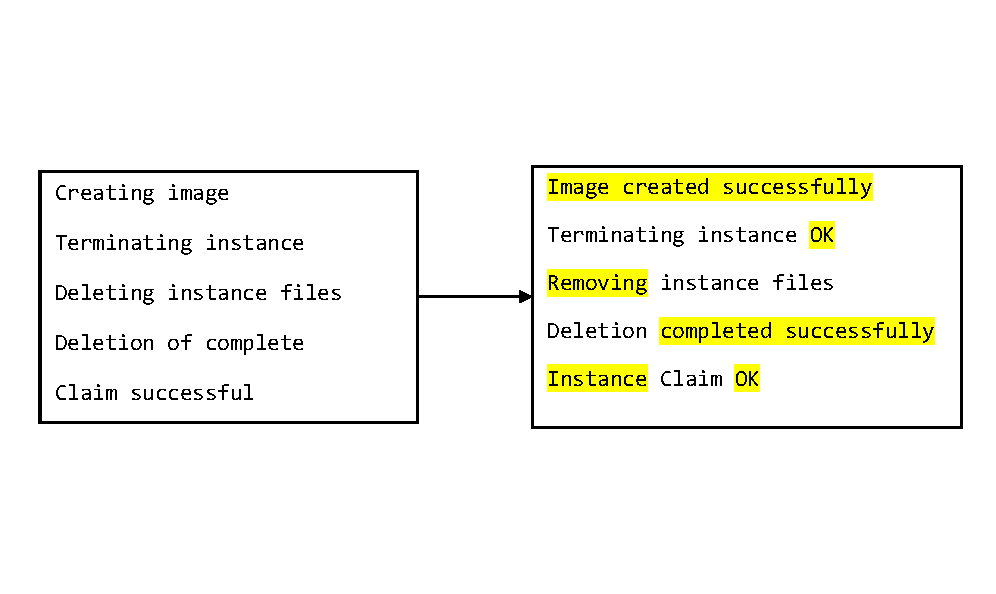
\includegraphics[width=11cm]{transfer_modifications.pdf}\\
  \caption{Changes on templates of the original dataset.}
  \label{fig:transfer_modifications}
\end{figure}




\section{Evaluation\label{sec:evaluation}}
In this section, the results of the evaluation between the two anomaly detection approaches, namely the regression-based approach and the classification-based approach are compared using three different language models, namely Bert, XL-Transformers and GPT-2. The pre-processing steps string cleansing and finetuning, as described \ref{sec:pre_processing} are investigated with regards to their potential on benefiting the quality of the word embeddings. Subsequently, the results of the evaluation using one dataset and the transfer of knowledge approach are presented.

\subsection{String cleansing}
String cleansing, as described in \ref{sec:template_cleansing}, can potentially  improve distinguishability between templates drastically in the used dataset.
For Bert, the pairwise cosine distances before cleansing are depicted in figure \ref{fig:bert_before_cleansing}, after cleansing in figure \ref{fig:bert_after_cleansing}. The corresponding templates to the indices on the x and y axes before and after cleansing can be found in table \ref{tab:templates_before_cleansing} and table \ref{tab:templates_after_cleansing} respectively.
The cosine distances before and after cleansing for GPT-2 can be found in figure \ref{fig:gpt_before_cleansing} and figure \ref{fig:gpt_after_cleansing}, and for XL-Transformer in figure \ref{fig:xl_before_cleansing} and figure \ref{fig:xl_after_cleansing}, respectively. The average pairwise cosine distances between templates before and after cleansing can be seen in table \ref{tab:average_pairwise_cos_distances}.
Note that the cosine distances between templates appear to be relatively low for GPT-2 before and after cleansing. Even though cleansing results in a two-fold increase in the distances, the initial value is already very low. We can see how the distinguishability between templates increases for Bert and even more impressively for XL-Transformers. While Bert has a slightly higher average pairwise cosine distance before cleansing, XL-Transformers highly benefits from cleansing with an average value of 0.62. This underlines the importance of this step in order to meet the requirements postulated in \ref{sec:word_vectorization}, depending on the deployed language models.



\begin{table}[ht]
\centering
\begin{small}
\begin{tabular}{ p{1.3cm} p{2.5cm} p{2.5cm} }
\toprule
Model & Before cleansing & After cleansing\\
\midrule
XL & 0.2511 & 0.7001\\
Bert & 0.2718 & 0.5004\\
GPT-2 & 0.0027 & 0.0053 \\ 

\bottomrule
\end{tabular}
\caption{Average pairwise template cosine distances.}
\label{tab:average_pairwise_cos_distances}
\end{small}
\end{table}


\begin{figure}[!tbp]
  \centering
  \subfloat[Before cleansing.]{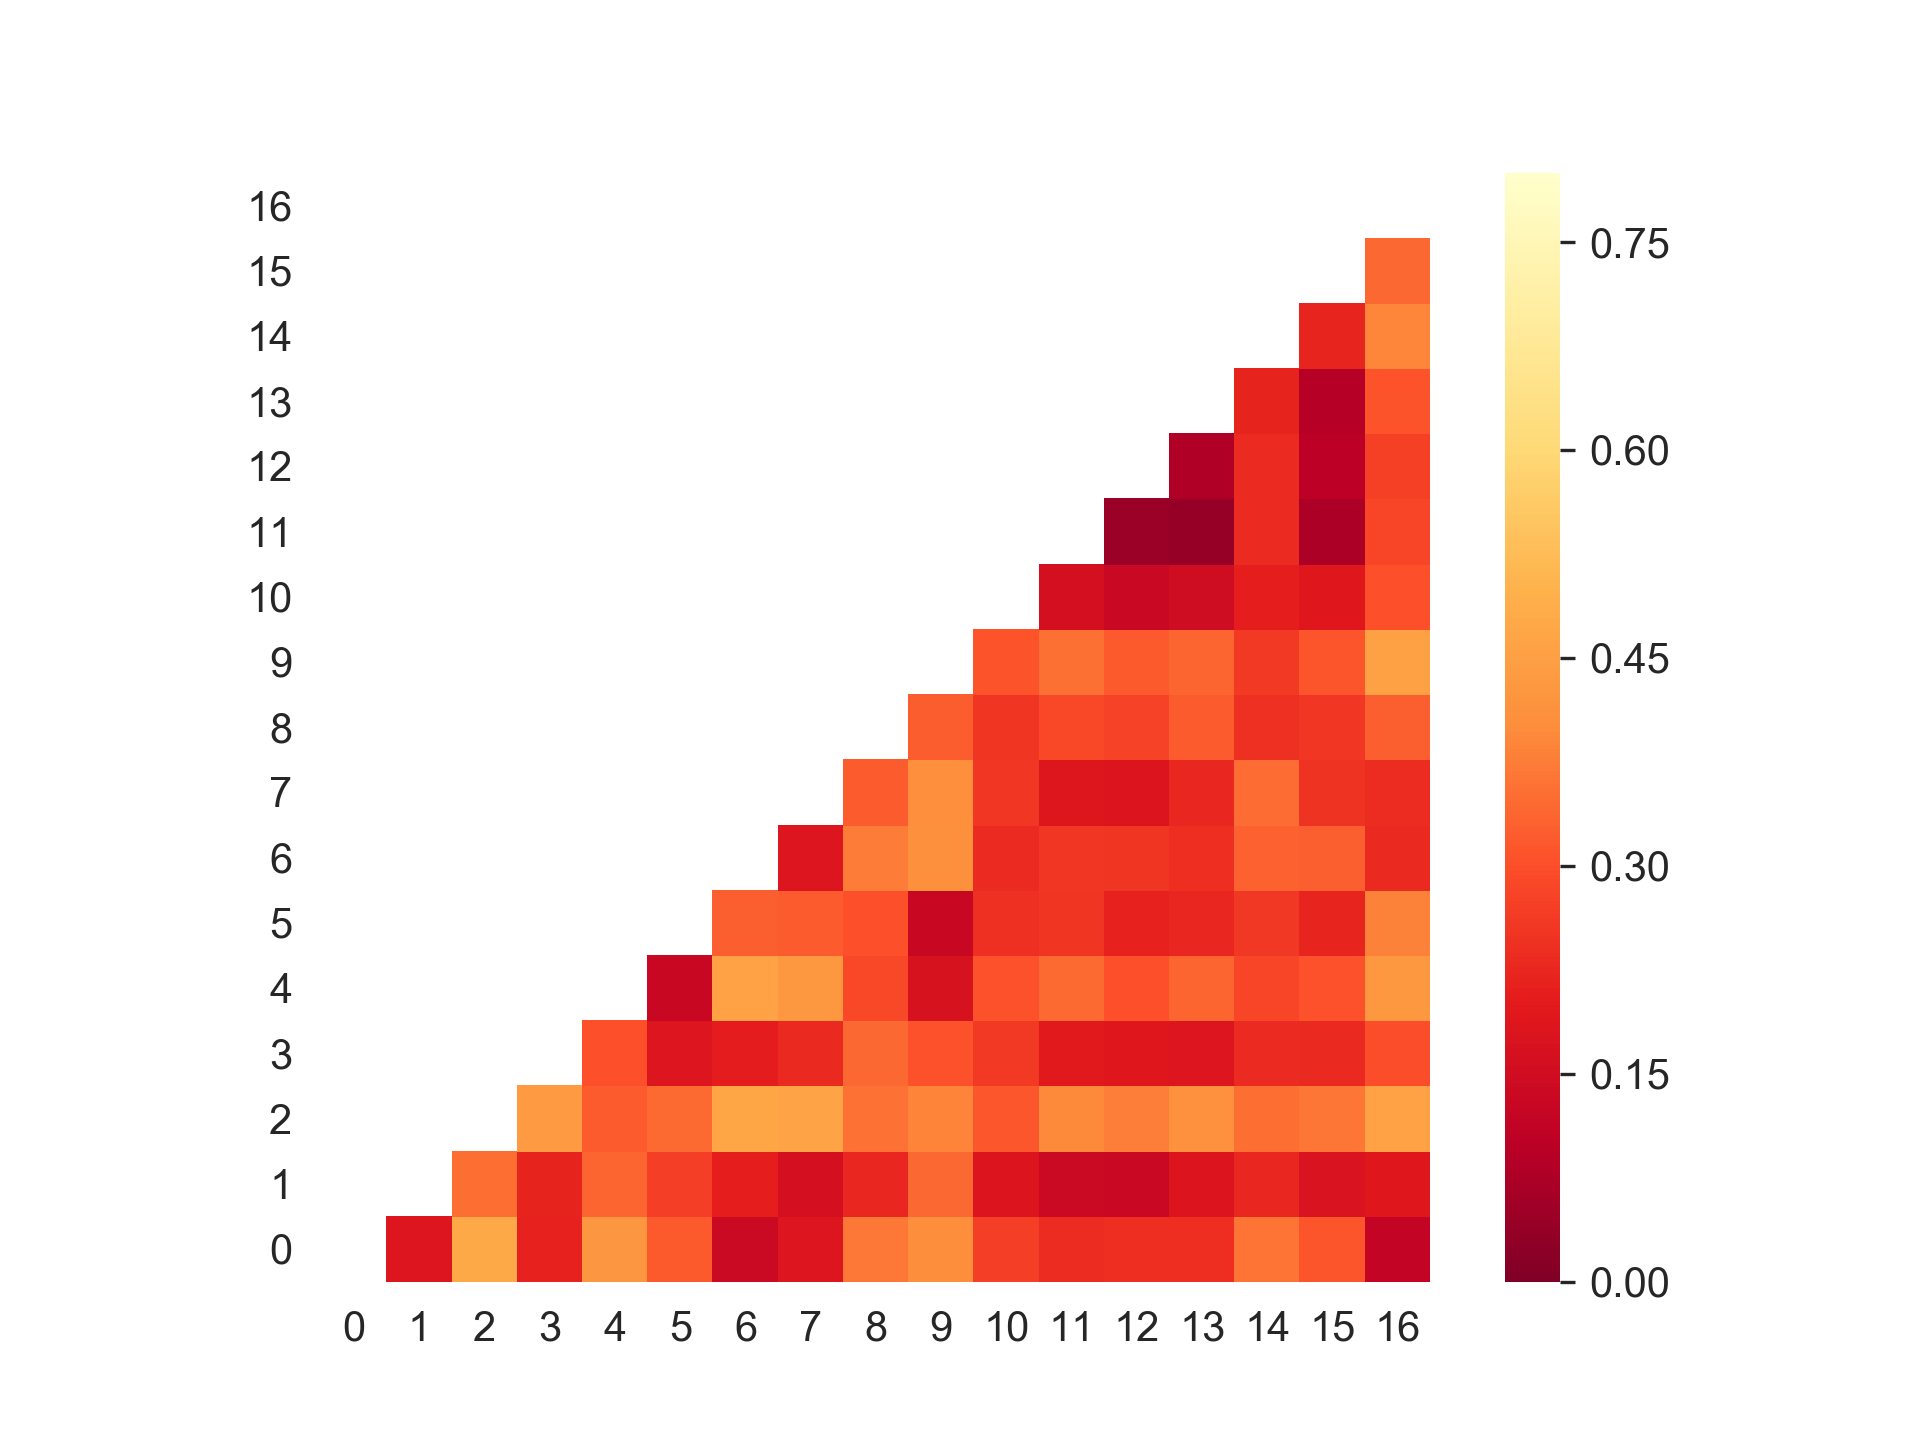
\includegraphics[width=0.48\textwidth]{bert_before_cleansing.png}\label{fig:bert_before_cleansing}}
  \hfill
  \subfloat[After cleansing.]{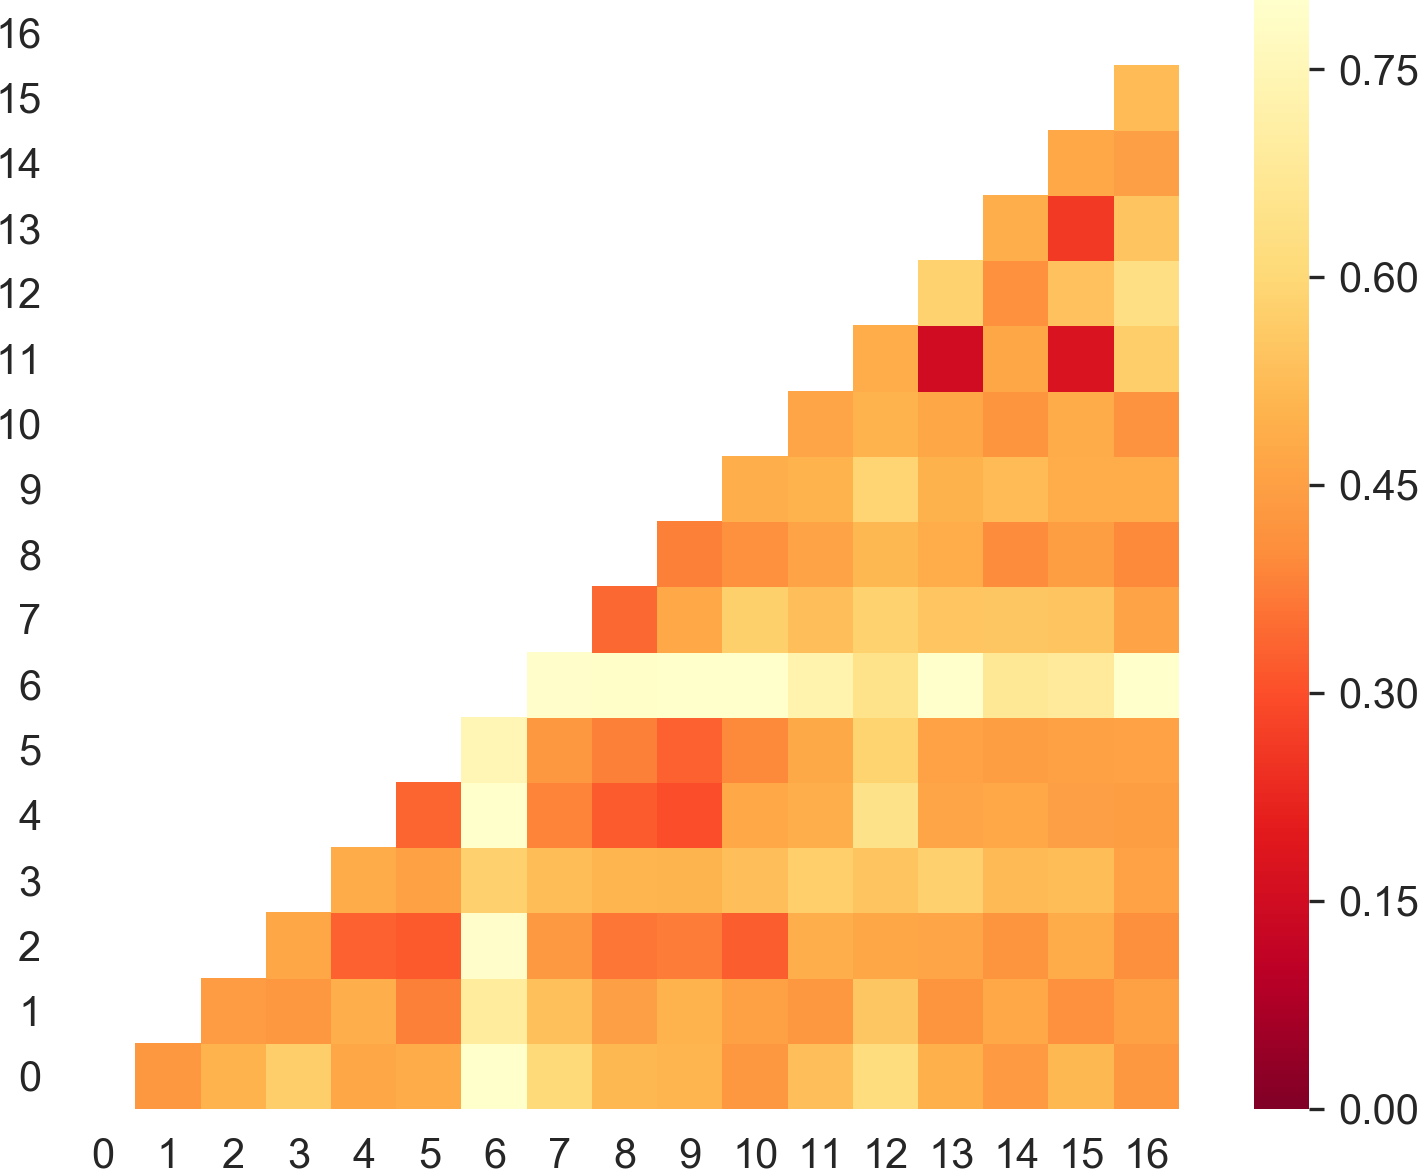
\includegraphics[width=0.48\textwidth]{bert_after_cleansing.png}\label{fig:bert_after_cleansing}}
  \caption{Bert pairwise template cosine distance.}
\end{figure}

\begin{figure}[!tbp]
  \centering
  \subfloat[Before cleansing.]{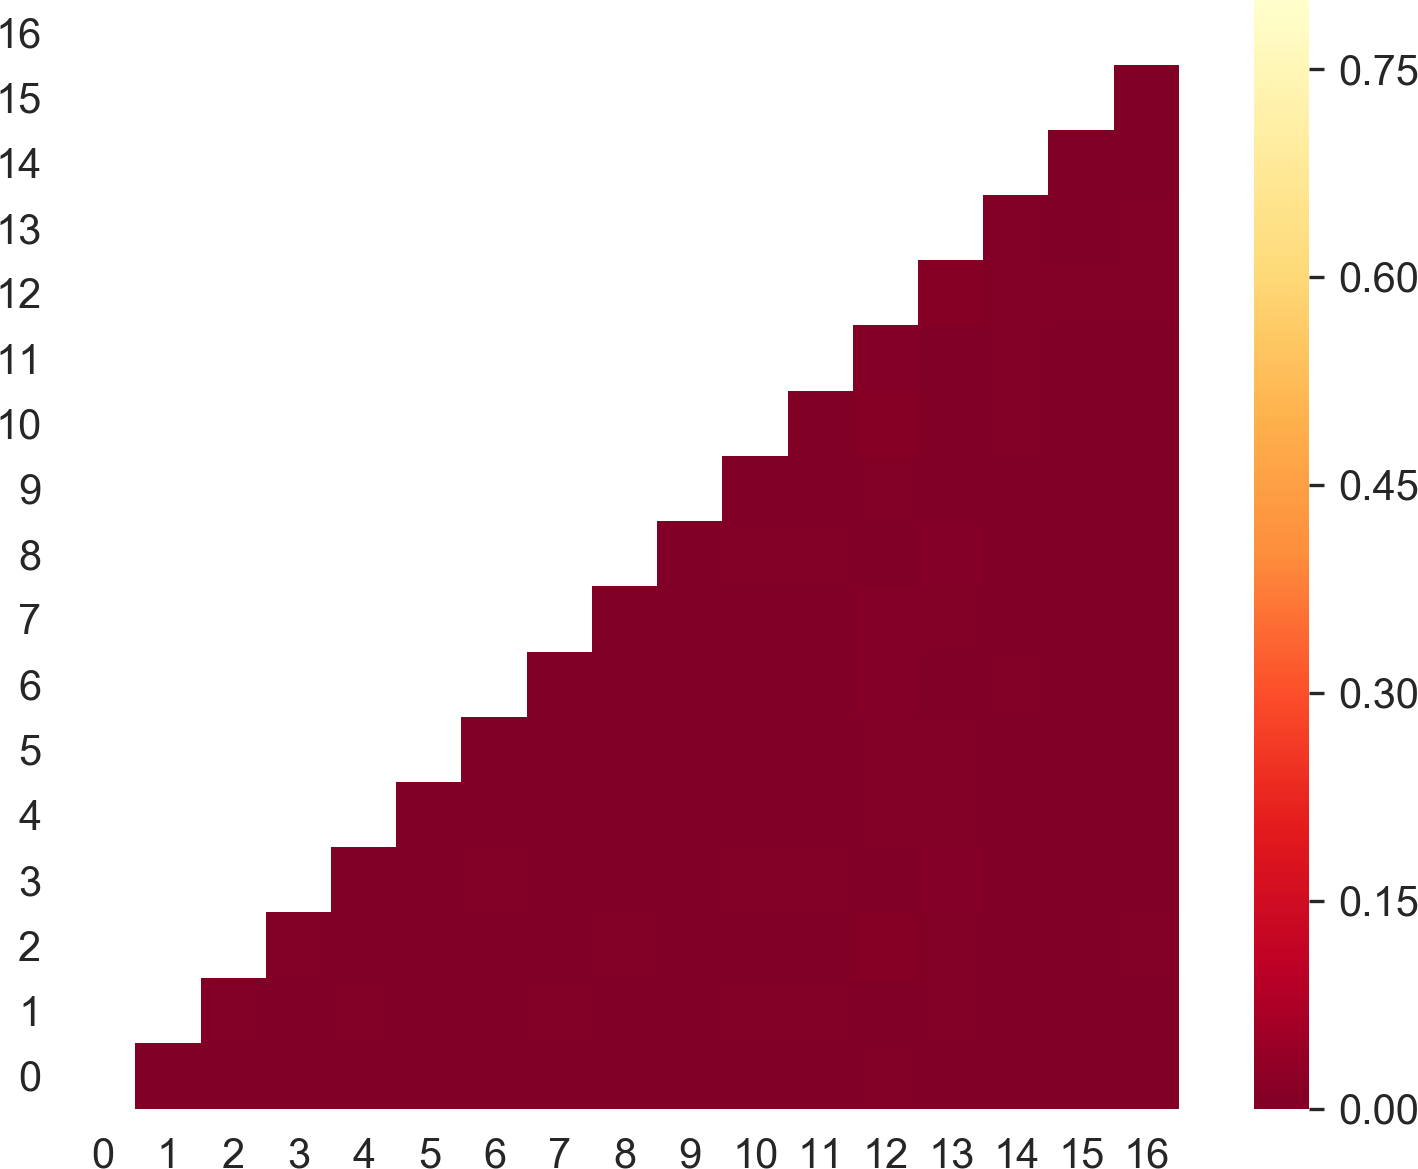
\includegraphics[width=0.48\textwidth]{gpt_before_cleansing.png}\label{fig:gpt_before_cleansing}}
  \hfill
  \subfloat[After cleansing.]{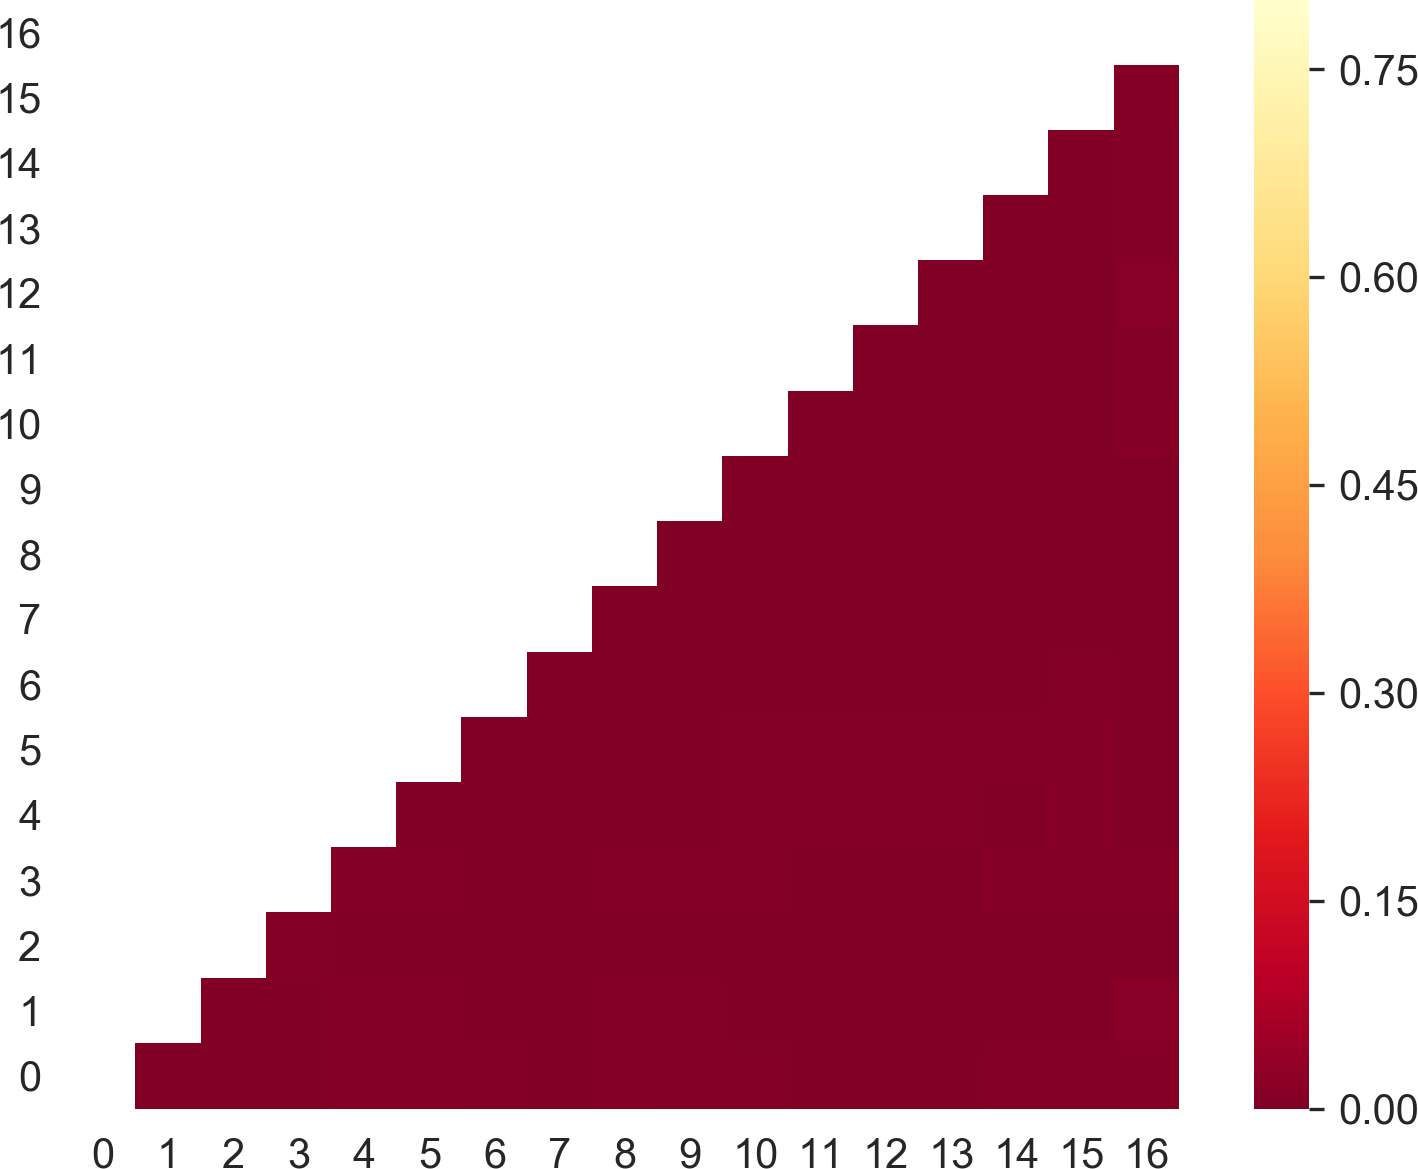
\includegraphics[width=0.48\textwidth]{gpt_after_cleansing.png}\label{fig:gpt_after_cleansing}}
  \caption{GPT-2 pairwise template cosine distance.}
\end{figure}

\begin{figure}[!tbp]
  \centering
  \subfloat[Before cleansing.]{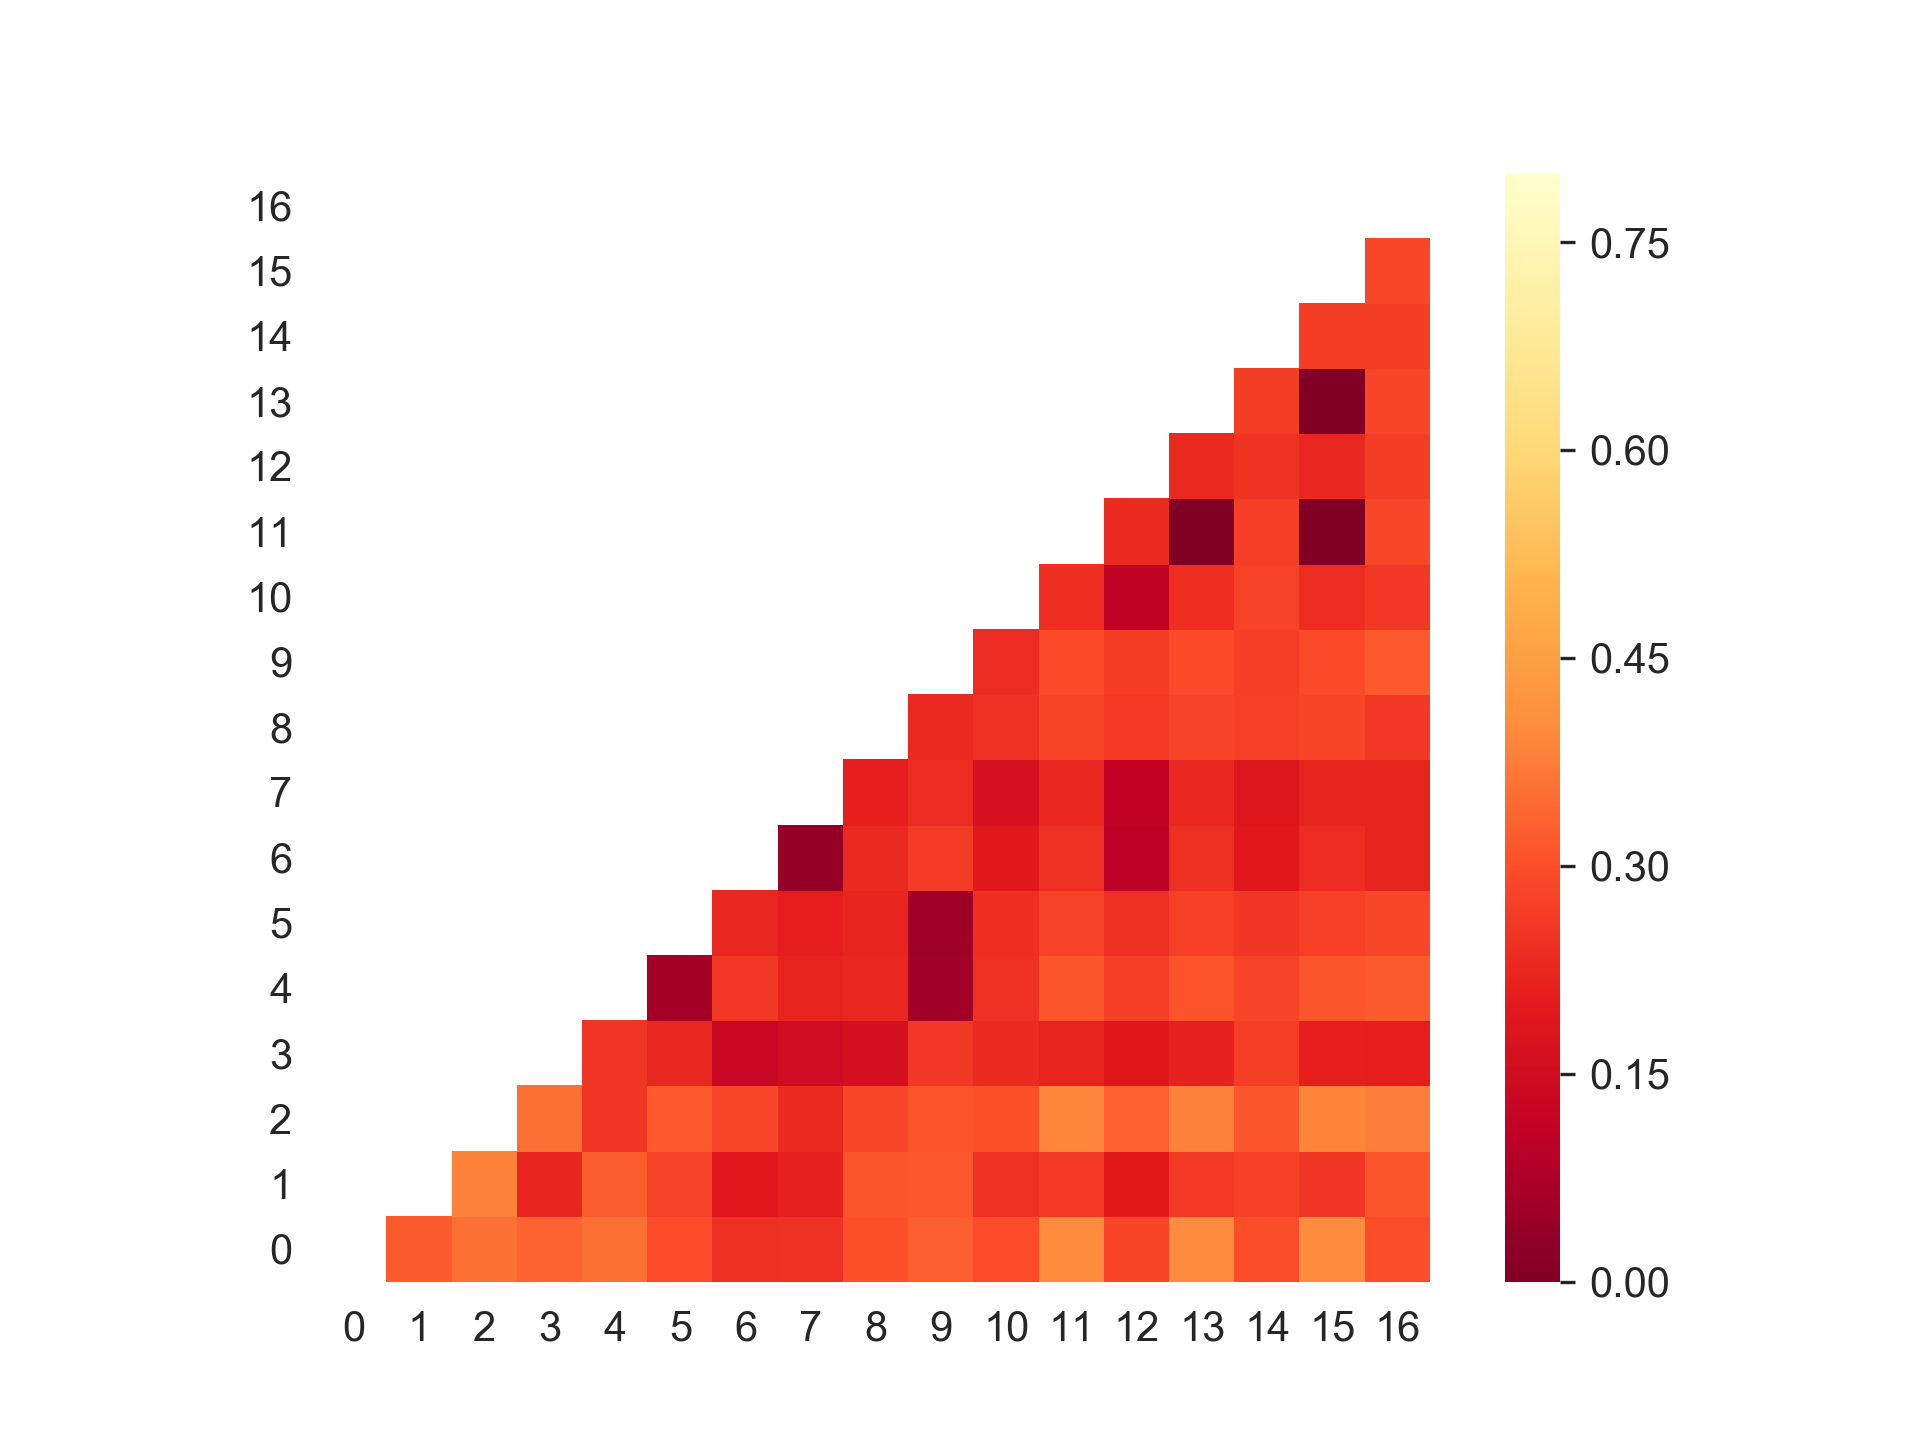
\includegraphics[width=0.48\textwidth]{xl_before_cleansing.png}\label{fig:xl_before_cleansing}}
  \hfill
  \subfloat[After cleansing.]{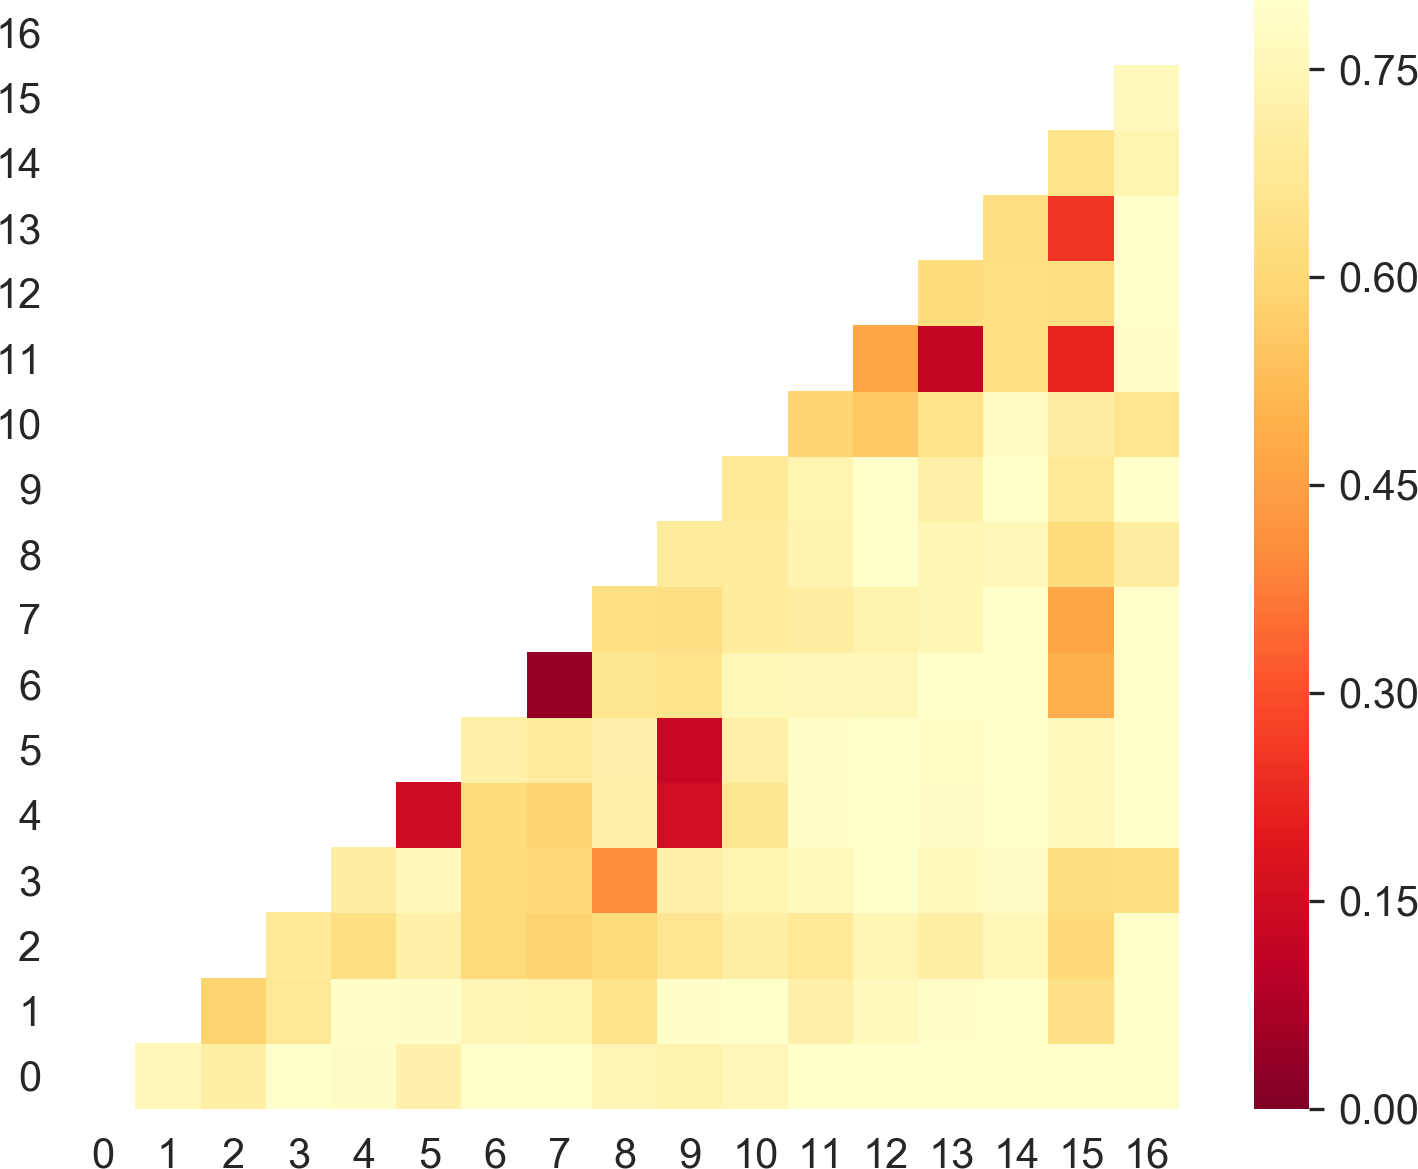
\includegraphics[width=0.48\textwidth]{xl_after_cleansing.png}\label{fig:xl_after_cleansing}}
  \caption{XL-Transformers pairwise template cosine distance.}
\end{figure}




\begin{table}[ht]
\begin{small}
\centering
\begin{tabular}{ c l } 
\toprule
Index & Template \\
\midrule
0 & $\langle*\rangle$ Creating image\\
1 & $\langle*\rangle$ VM $\langle*\rangle$ (Lifecycle Event)\\
2 & $\langle*\rangle$ During sync\_power\_state the instance has a pending task (spawning). Skip.\\
3 & $\langle*\rangle$ Instance $\langle*\rangle$ successfully.\\
4 & $\langle*\rangle$ Took $\langle*\rangle$.$\langle*\rangle$ seconds to $\langle*\rangle$ the instance on the hypervisor.\\
5 & $\langle*\rangle$ Took $\langle*\rangle$.$\langle*\rangle$ seconds to build instance.\\
6 & $\langle*\rangle$ Terminating instance\\
7 & $\langle*\rangle$ Deleting instance files $\langle*\rangle$\\
8 & $\langle*\rangle$ Deletion of $\langle*\rangle$ complete\\
9 & $\langle*\rangle$ Took $\langle*\rangle$.$\langle*\rangle$ seconds to deallocate network for instance.\\
10 & $\langle*\rangle$ Attempting claim: memory $\langle*\rangle$ MB, disk $\langle*\rangle$ GB, vcpus $\langle*\rangle$ CPU\\
11 & $\langle*\rangle$ Total memory: $\langle*\rangle$ MB, used: $\langle*\rangle$.$\langle*\rangle$ MB\\
12 & $\langle*\rangle$ memory limit: $\langle*\rangle$.$\langle*\rangle$ MB, free: $\langle*\rangle$.$\langle*\rangle$ MB\\
13 & $\langle*\rangle$ Total disk: $\langle*\rangle$ GB, used: $\langle*\rangle$.$\langle*\rangle$ GB\\
14 & $\langle*\rangle$ $\langle*\rangle$ limit not specified, defaulting to unlimited\\
15 & $\langle*\rangle$ Total vcpu: $\langle*\rangle$ VCPU, used: $\langle*\rangle$.$\langle*\rangle$ VCPU\\
16 & $\langle*\rangle$ Claim successful\\
\bottomrule
\end{tabular}
\caption{Templates before cleansing}
\label{tab:templates_before_cleansing}
\end{small}
\end{table}



\begin{table}[ht]
\begin{small}
\centering
\begin{tabular}{ c l } 
\toprule
Index & Template \\
\midrule
0 & Creating image\\
1 & VM  Lifecycle Event\\
2 & During sync power state the instance has a pending task spawning Skip\\
3 & Instance  successfully\\
4 & Took  seconds to  the instance on the hypervisor\\
5 & Took  seconds to build instance\\
6 & Terminating instance\\
7 & Deleting instance files\\
8 & Deletion of complete\\
9 & Took  seconds to deallocate network for instance\\
10 & Attempting claim memory  MB disk  GB vcpus  CPU\\
11 & Total memory  MB used  MB\\
12 & memory limit  MB free  MB\\
13 & Total disk  GB used  GB\\
14 & limit not specified defaulting to unlimited\\
15 & Total vcpu  VCPU used  VCPU\\
16 & Claim successful\\
\bottomrule
\end{tabular}
\caption{Templates after cleansing}
\label{tab:templates_after_cleansing}
\end{small}
\end{table}

\clearpage
\subsection{Finetuning}
As described in \ref{sec:finetuning}, finetuning can potentially help to produce word embeddings that are more adequate for solving a certain task, it is thus desirable to produce word embeddings that help solving the task of anomaly detection better. As described in \ref{sec:word_vectorization}, a high cosine distance between semantically different templates is required. The dataset that consists of the templates in table \ref{tab:templates_after_cleansing} has been chosen for finetuning. Since the pre-trained language models at hand (namely \textit{bert-base-uncased} and \textit{gpt2}) have been trained on a large corpus, finetuning would also need to be executed on a sufficiently large corpus. Since this is not the case, the results of finetuning for a maximum of four epochs, as suggested by the Bert authors \cite{devlin2018bert}, does not yield the desired results. As it can be seen in figure \ref{fig:cos_distance_finetuning}, it was not possible to increase the cosine distances between templates on the task of Masked LM (as described in \ref{Bert}), compared to the cosine distances depicted in figure \ref{fig:bert_after_cleansing}. The average distance between templates dropped to 0.3016 from 0.4449. The fact that the loss on the evaluation part of the dataset is not decreasing adequately, as shown in figure \ref{fig:finetuning_loss}, shows that training on such a small corpus is not able to generalise well enough, which makes finetuning on the default learning task not useful in this case. Since the Huggingface Transformers library does not offer out of the box finetuning interfaces for GPT-2 and XL-Transformers on the same task as for Bert, they are not further investigated for finetuning.

\begin{figure}[H]
  \centering
  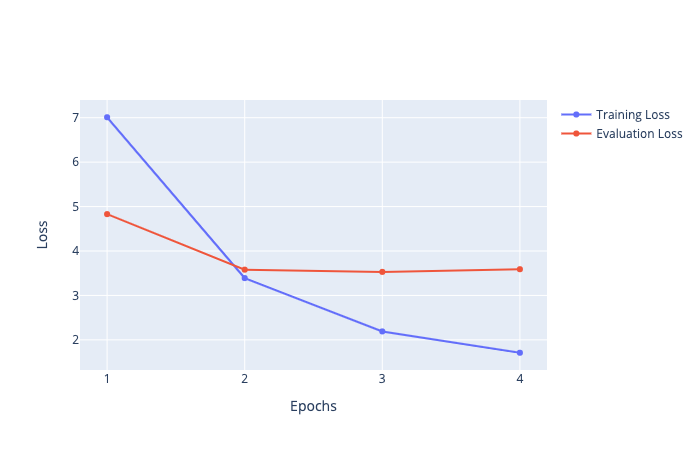
\includegraphics[width=12cm,height=8.5cm]{finetuning_loss.png}\\
  \caption{Training and evaluation loss for finetuning on masked LM.}
  \label{fig:finetuning_loss}
\end{figure}

\begin{figure}[h]
  \centering
  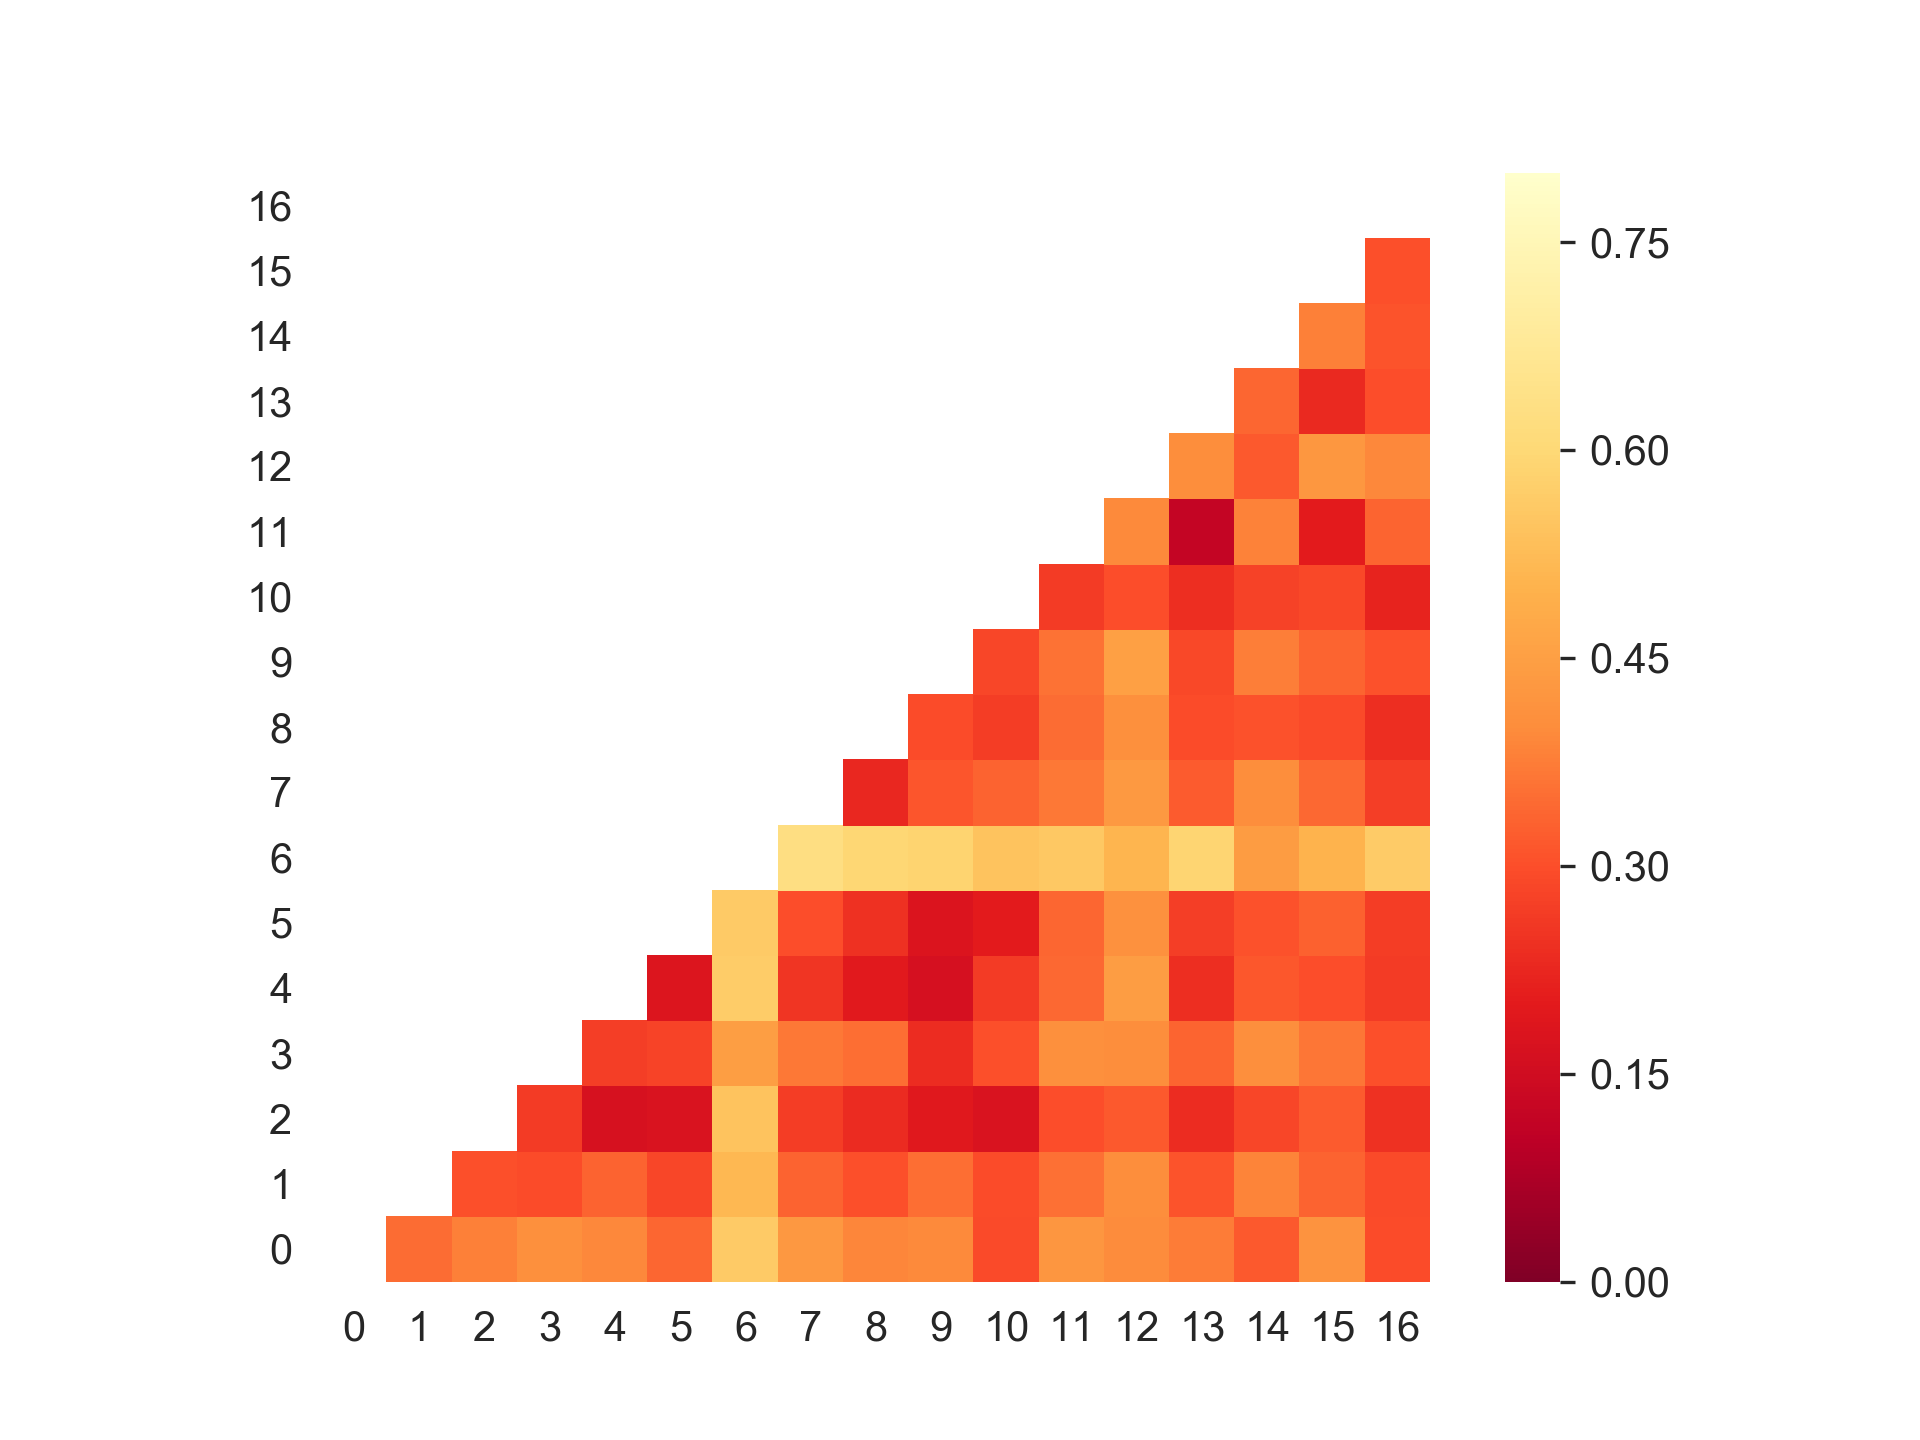
\includegraphics[width=12cm,height=9cm]{bert_finetuning_cleansed.png}\\
  \caption{Cosine distance between templates after cleansing and finetuning}
  \label{fig:cos_distance_finetuning}
\end{figure}


\subsection{Hyperparameters}
In order to find well-suited parameters for the LSTM model, it was first applied to the problem using a minimal configuration. With the help of a grid-search, running simulations with different configurations, the following hyperparameters have proven to yield the most satisfying results:
\begin{itemize}
	\item 512 hidden units for the bidirectional LSTM, with one layer
	\item two fully connected layers with 512 units $\rightarrow$ 256 units $\rightarrow$ output size
	\item dropout of 0.1 between every layer
	\item input sequence length of 7
	\item 60 Epochs of training
\end{itemize}

%%%%%%%%%%%%
% REGRESSION 
%%%%%%%%%%%%
\subsection{Regression-based approach using one dataset\label{sec:results-regression}}
In this subsection, the results of the regression-based approach, with various alterations using the different language models are presented. In order to evaluate the robustness of the language models to the evolution of log events, alterations as described in \ref{sec:logs_alteration} are injected at different ratios. The impact on detecting anomalies after alterations on the sequence of logs are injected, i.e. deleting, shuffling and duplicating events are summarised in figure \ref{fig:results_regression_sequential}. Alterations are not injected all at the same time, but independently from each other, the results in the figures are average values of all experiments with alterations on the log sequences. Results broken down by each alteration can be found in the appendix \ref{appendix:regression}. From 5\% to 15\% alterations, both Bert and GPT-2 show perfect recall values of 1.0, while XL-Transformers is only able to detect 61\% to 65\% of all anomalies. With regards to precision, GPT-2 reaches values from 0.91 for 5\% alterations to 1.0 for 10\% alterations to 0.88 for 15\% alterations, while Bert declines from 0.55 at 5\% alterations to 0.43 with 15\% alterations. XL-Transformers in turn returns very low values of 0.32 for 5\% alterations to 0.21 for 15\% alterations. Also for F1-score, GPT-2 achieves very good results with about 0.95 for all alteration ratios, while Bert declines from 0.69 for 5\% alterations to 0.56 for 15\% alterations. XL-Transformers performs comparably bad as for the other metrics. It is evident, that GPT-2 performs better than Bert and XL-Transformers with all metrics in this category, except for recall, where Bert is performing equally well. Bert can be located as second place in this category, while XL-Transformers delivers the least satisfying results in comparison to Bert and GPT-2.

In addition to the alterations on the log sequences, alterations on the log events themselves, i.e. inserting, removing and replacing words are also of interest. The results of this experiment can be seen in figure \ref{fig:results_regression_words}. Again, the alterations are not injected all at once, but independently - the figure shows averaged results. Exactly as for the previous results, we can see that both Bert and GPT-2 show a perfect for performance with regards to recall, which is 1.0 overall for all alteration ratios, while XL-Transformers delivers results of around 0.63. GPT-2 performs equally good on both F1-score and precision as in the previous experiments, while Bert shows values for F1-score which are between 8 and 10 percentage points better, and for precision also results that improved around 7 percentage points. XL-Transformers shows even higher improvements than Bert, with an average improvement of 13 percentage points for F1-score and an average improvement of 0.17 for precision, with a slight degradation in recall of 0.03 on average. Again, GPT-2 shows the best results overall, followed by Bert and XL-Transformers.

The result of replacing 50\% of the words in 15\% of the log lines, where the lines containing replacements are expected to be marked as an anomaly by the model, can be see in figure \ref{fig:replace_words_regression}. It is clearly visible that this experiment shows a different picture as the previous ones, with GPT-2 showing weak results, while Bert and especially XL-Transformers showing partly better results than they did previously. Bert achieves a F1-score of 0.71, XL-Transformers 0.6 and GPT-2 0.09. Also for precision the results are slightly better for Bert and XL-Transformers - Bert achieving 0.61, XL-Transformers 0.6, and GPT-2 0.13. XL-Transformers shows improvements for recall with 0.75, while Bert degrades to 0.86, and GPT-2 degrades to 0.07. This experiment, complementary to the previous ones, where an anomaly line was injected and GPT-2 achieved a high robustness, being able to detect injected anomalies well, shows that GPT-2 is not able to distinguish between normal log lines and 

Another aspect that is evaluated, is the impact of the input sequence length, i.e. the number of concatenated log events for which the next log event shall be predicted, on the ability of the model to detect anomalies. The results of this evaluation can be seen in \ref{fig:seq_len_regression}. Bert and GPT-2 seem to profit slightly from sequence lengths longer than 6 or 7, whereas the quality of results for XL-Transformers are not as affected from the input sequence length, but are generally lower.

\begin{comment}
\begin{figure}[h]
  \centering
  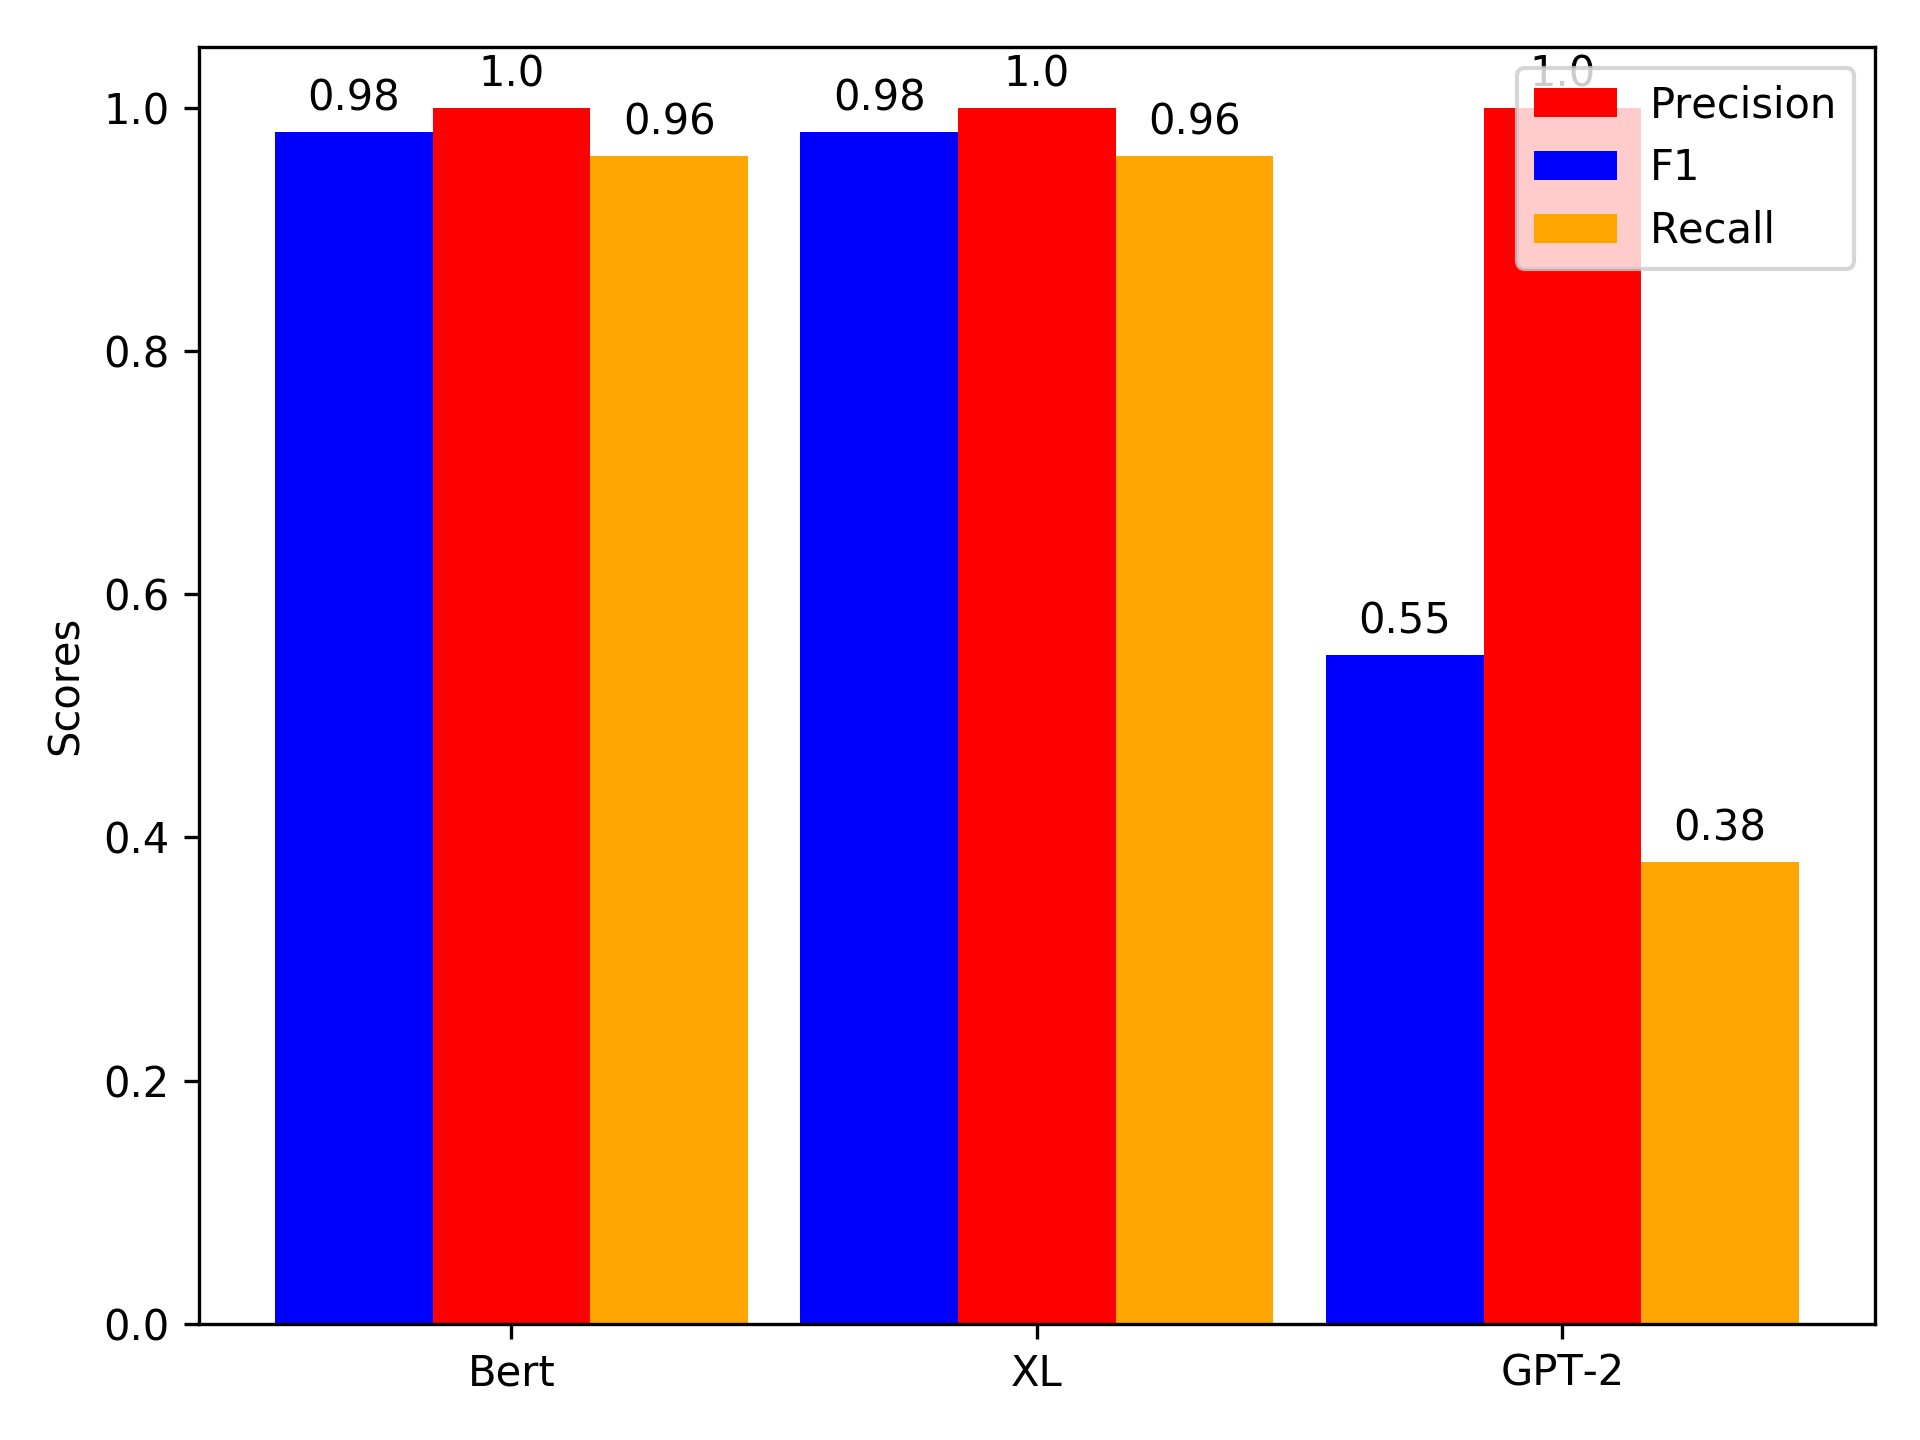
\includegraphics[width=6cm,height=4.5cm]{results/regression_sequence/regression_reverse.png}\\
  \caption{Scores for detecting reversed order of log events, using regression.}
  \label{fig:regression_reverse_order}
\end{figure}
\end{comment}

\begin{figure*}[ht!]
  \centering
  \captionsetup{justification=centering}
   \subfloat[5\% alteration\label{fig:results_regression_sequential_5}]{%
      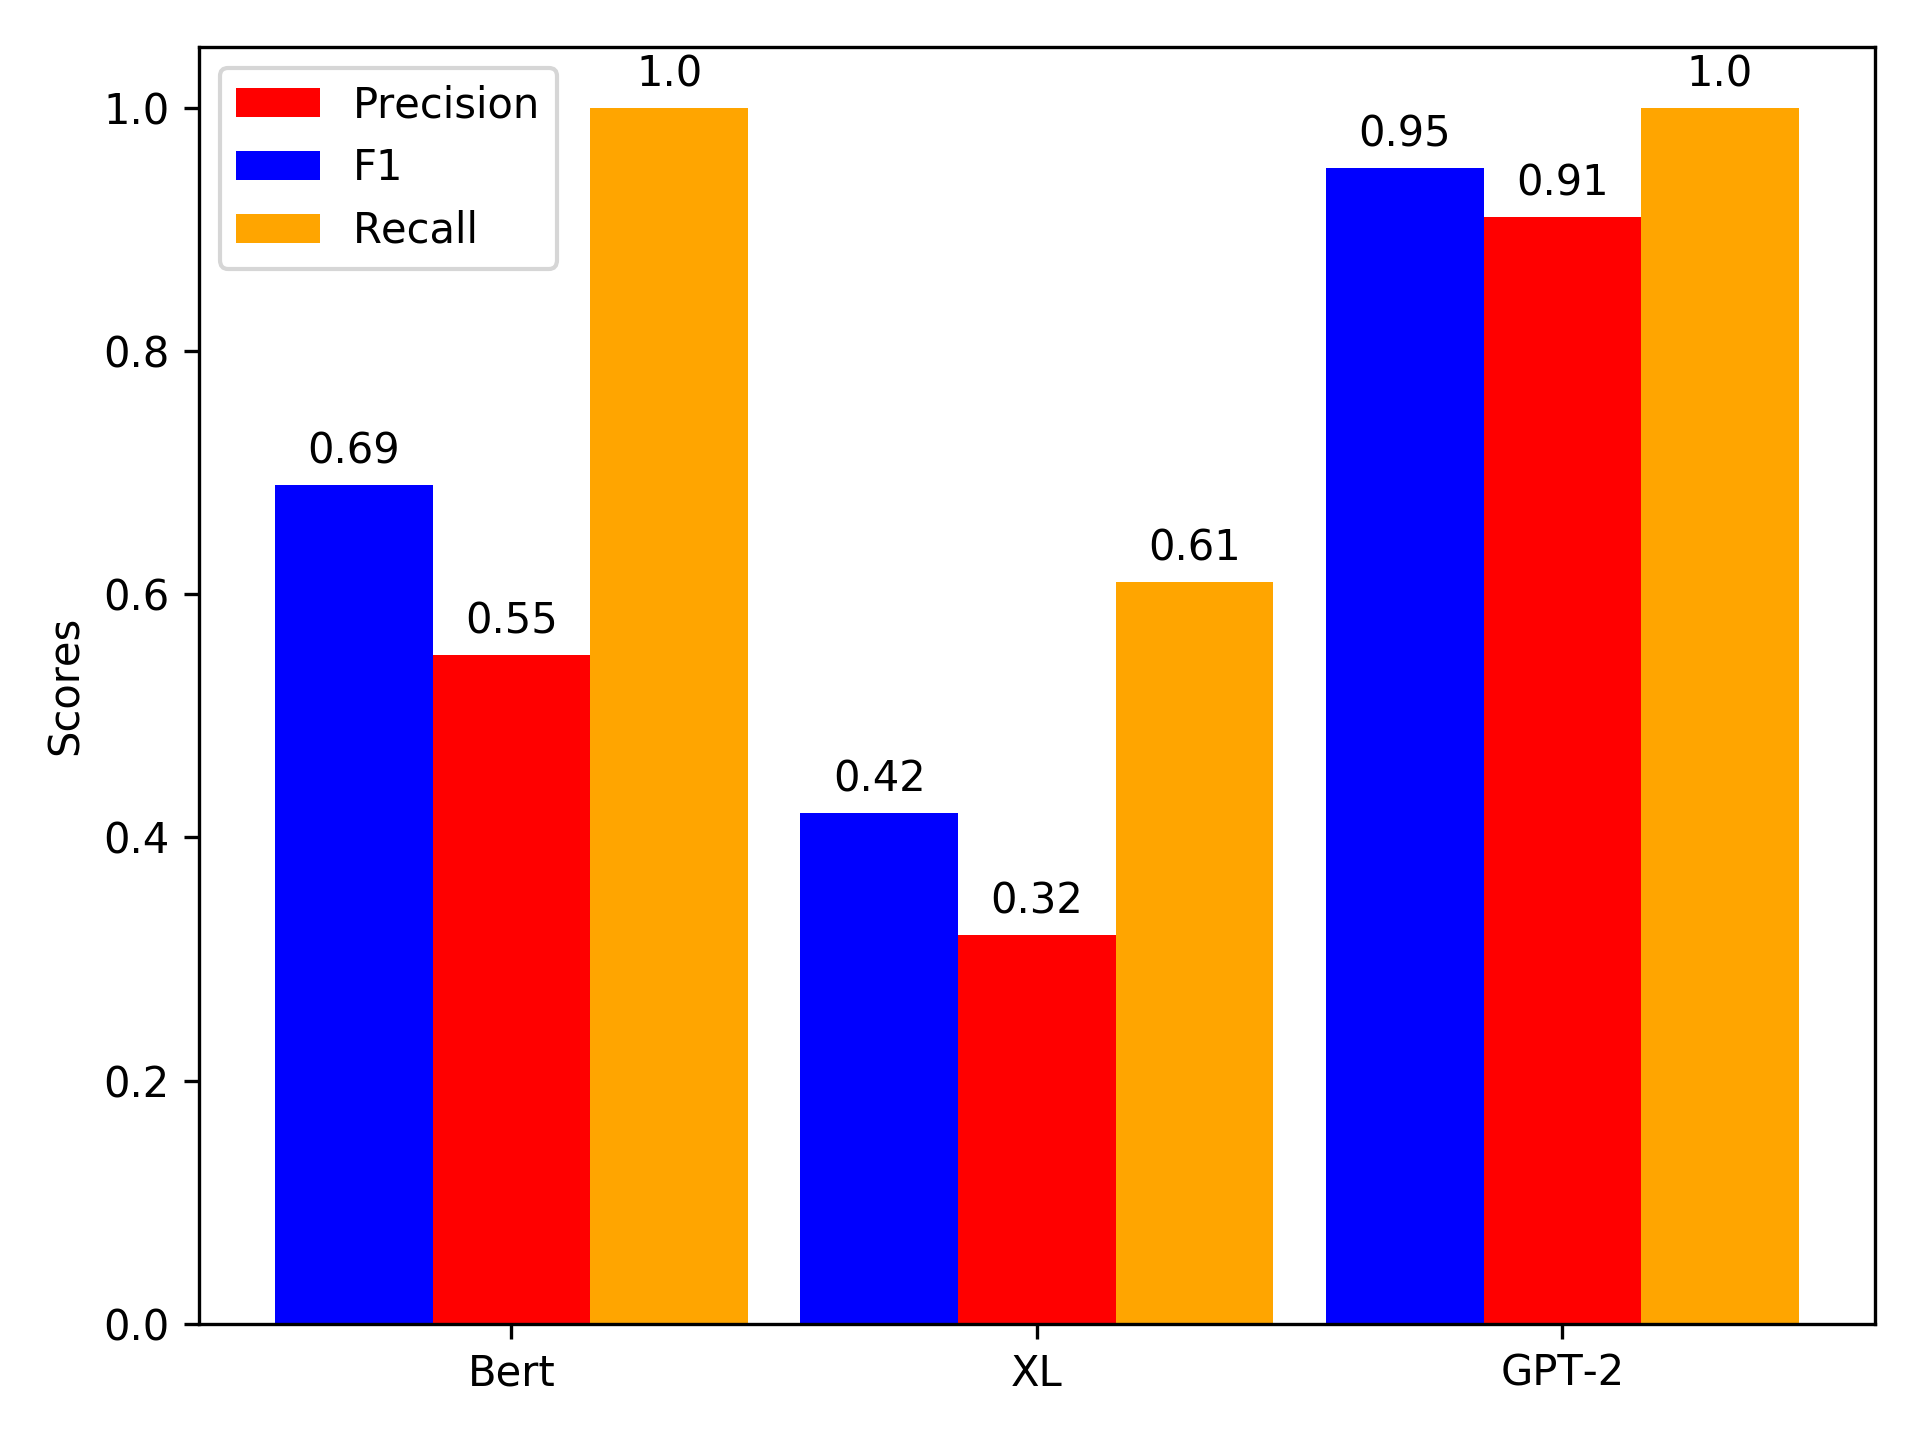
\includegraphics[trim={1cm 0.5cm 0cm 1cm}, width=0.322\textwidth]{results/average/regression_sequential_average_ratio_0.05.png}}
\hspace{\fill}
   \subfloat[10\% alteration\label{fig:results_regression_sequential_10} ]{%
      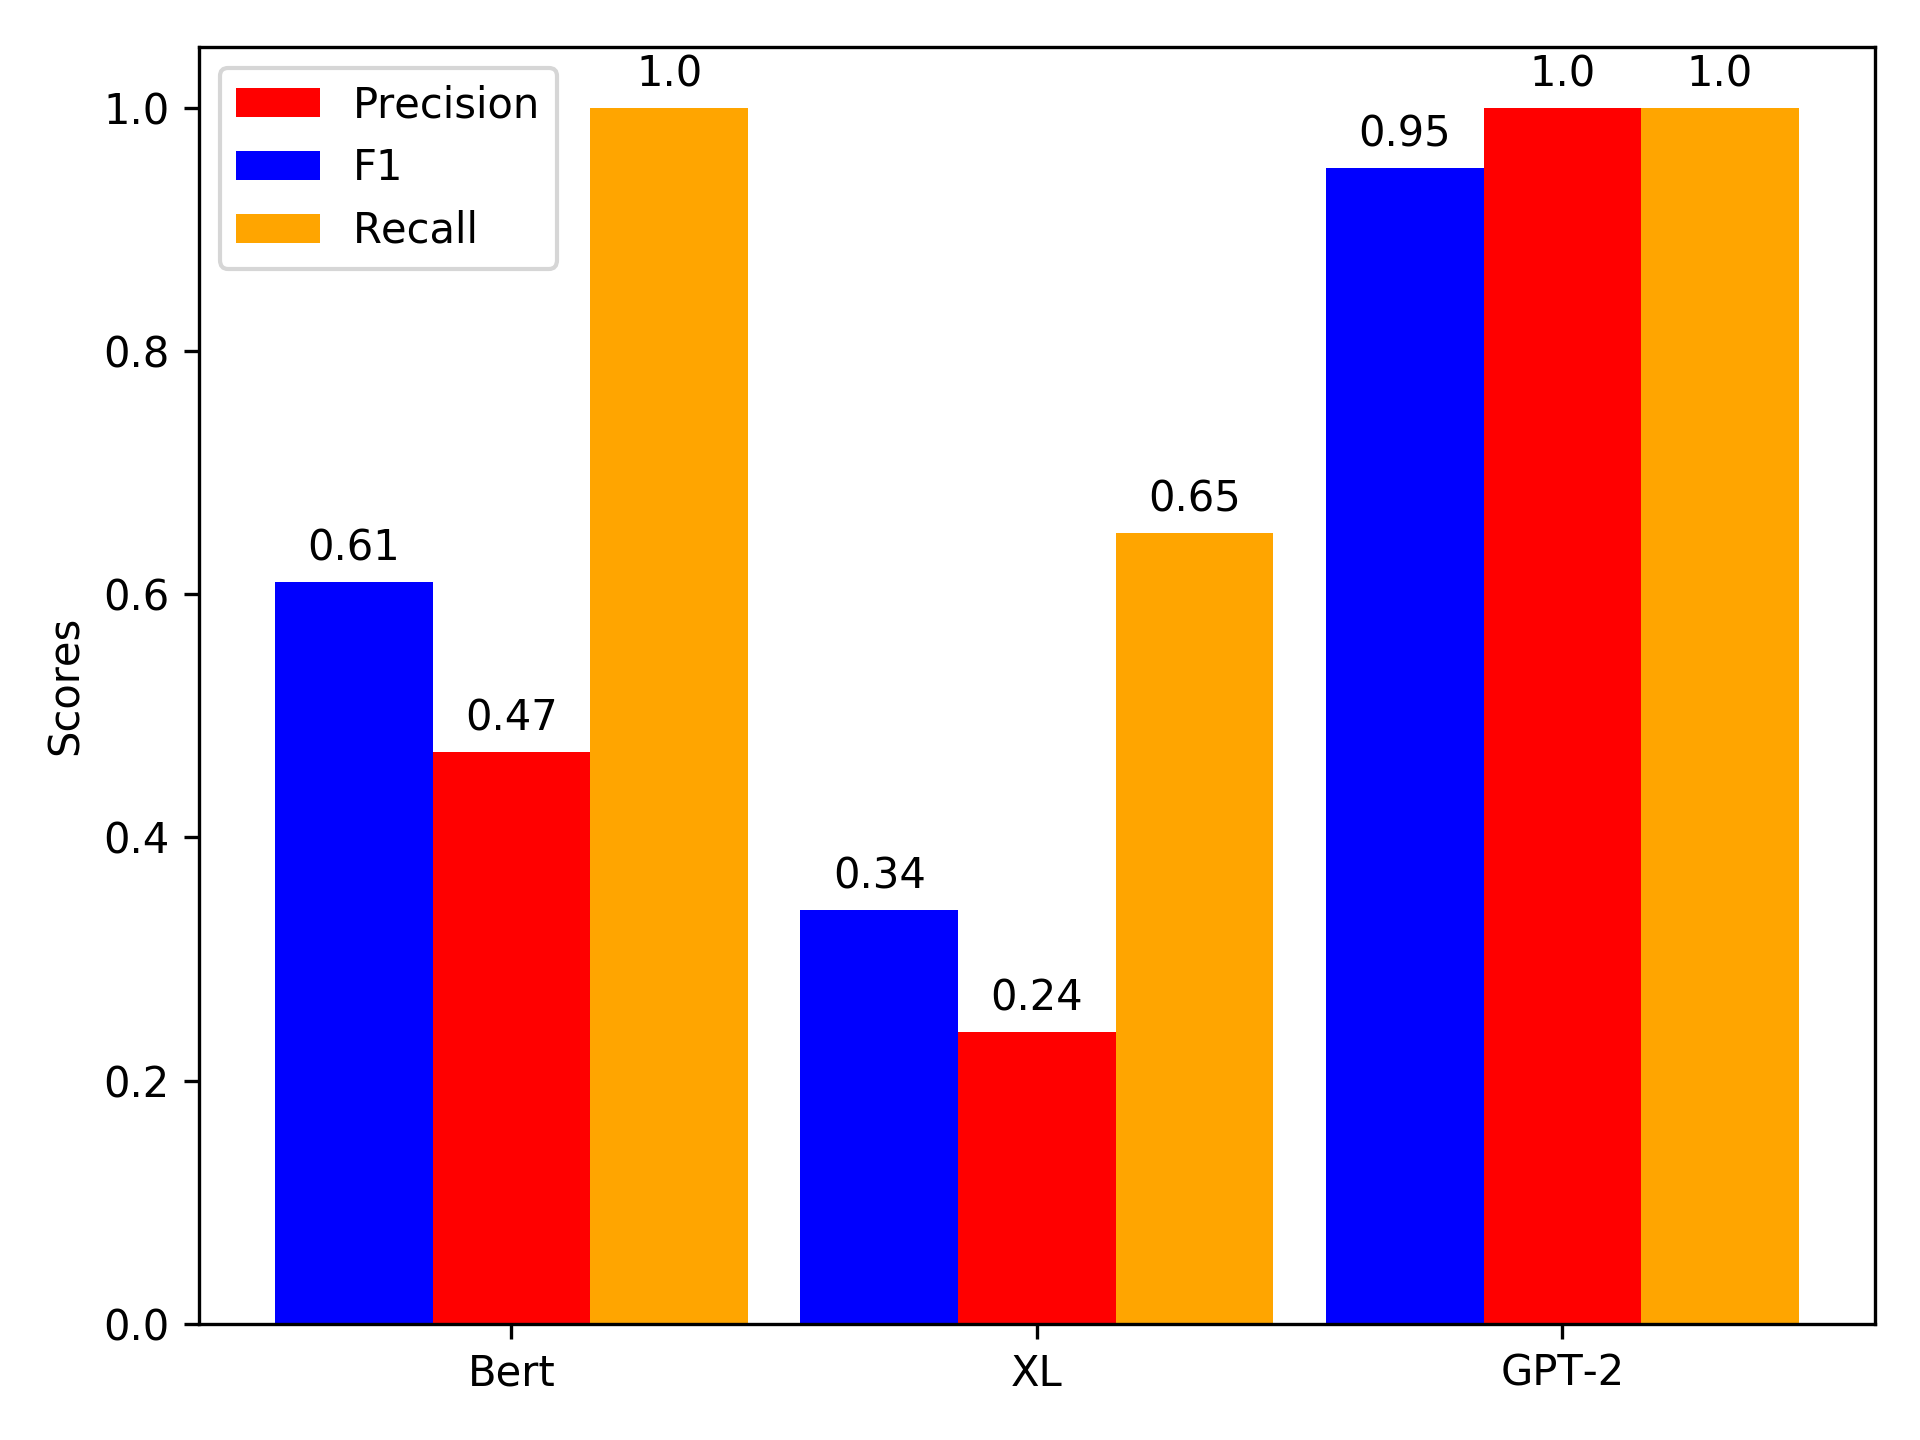
\includegraphics[trim={1cm 0.5cm 0cm 1cm}, width=0.322\textwidth]{results/average/regression_sequential_average_ratio_0.10.png}}
\hspace{\fill}
   \subfloat[15\% alteration\label{fig:results_regression_sequential_15}]{%
      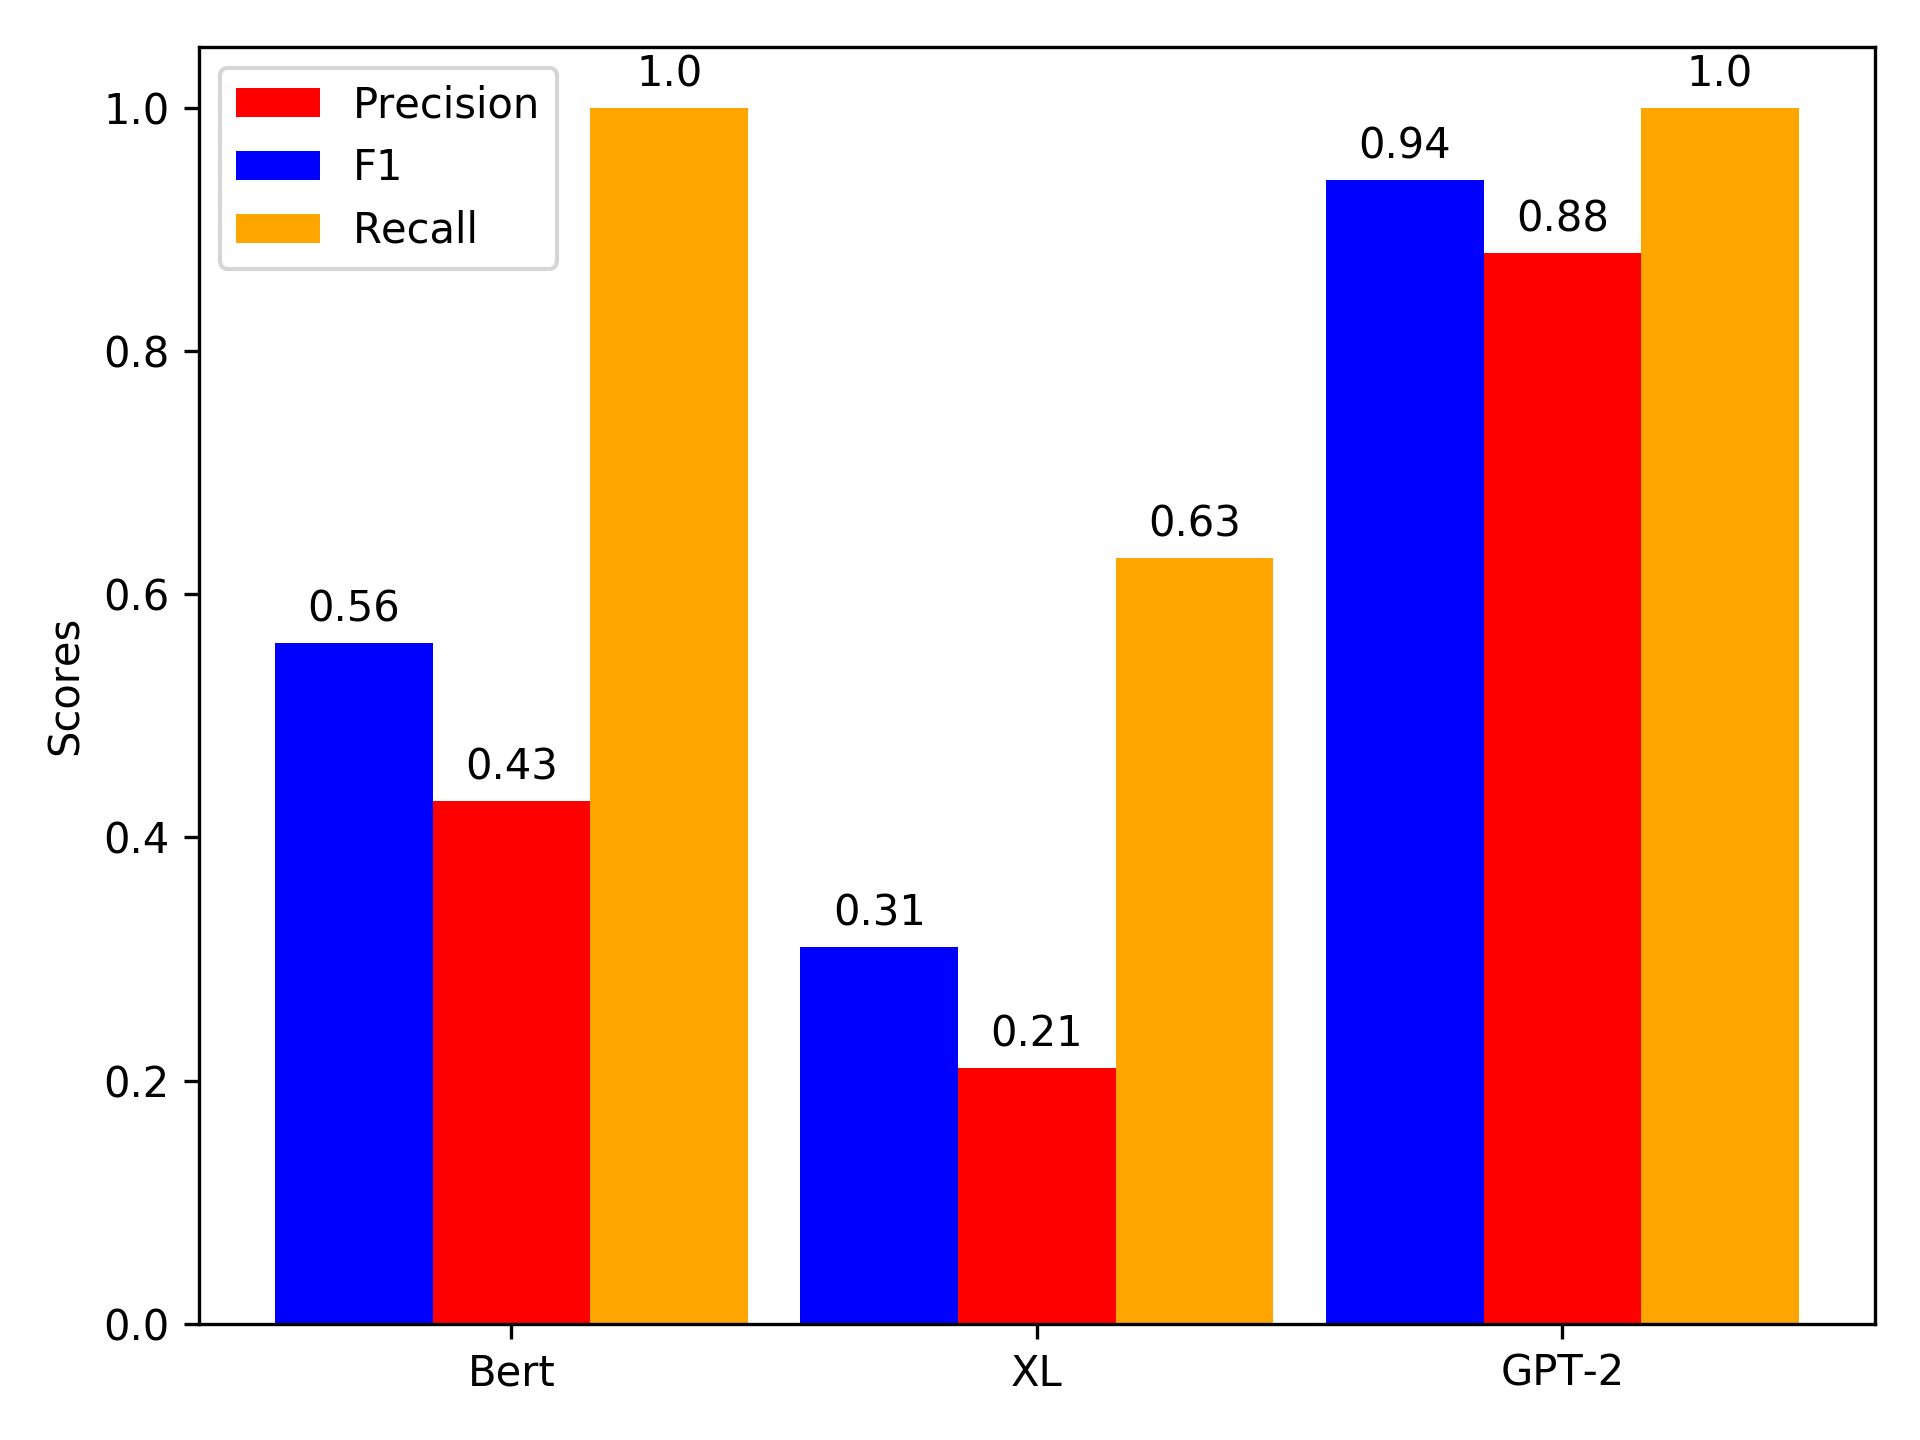
\includegraphics[trim={1cm 0.5cm 0cm 1cm}, width=0.322\textwidth]{results/average/regression_sequential_average_ratio_0.15.png}}\\
\caption{\label{fig:results_regression_sequential}Altering the sequences of logs at different ratios, 5\% anomalies, using regression.}
\end{figure*}


\begin{figure*}[ht!]
  \centering
  \captionsetup{justification=centering}
   \subfloat[5\% alteration\label{fig:results_regression_qualitative_5}]{%
      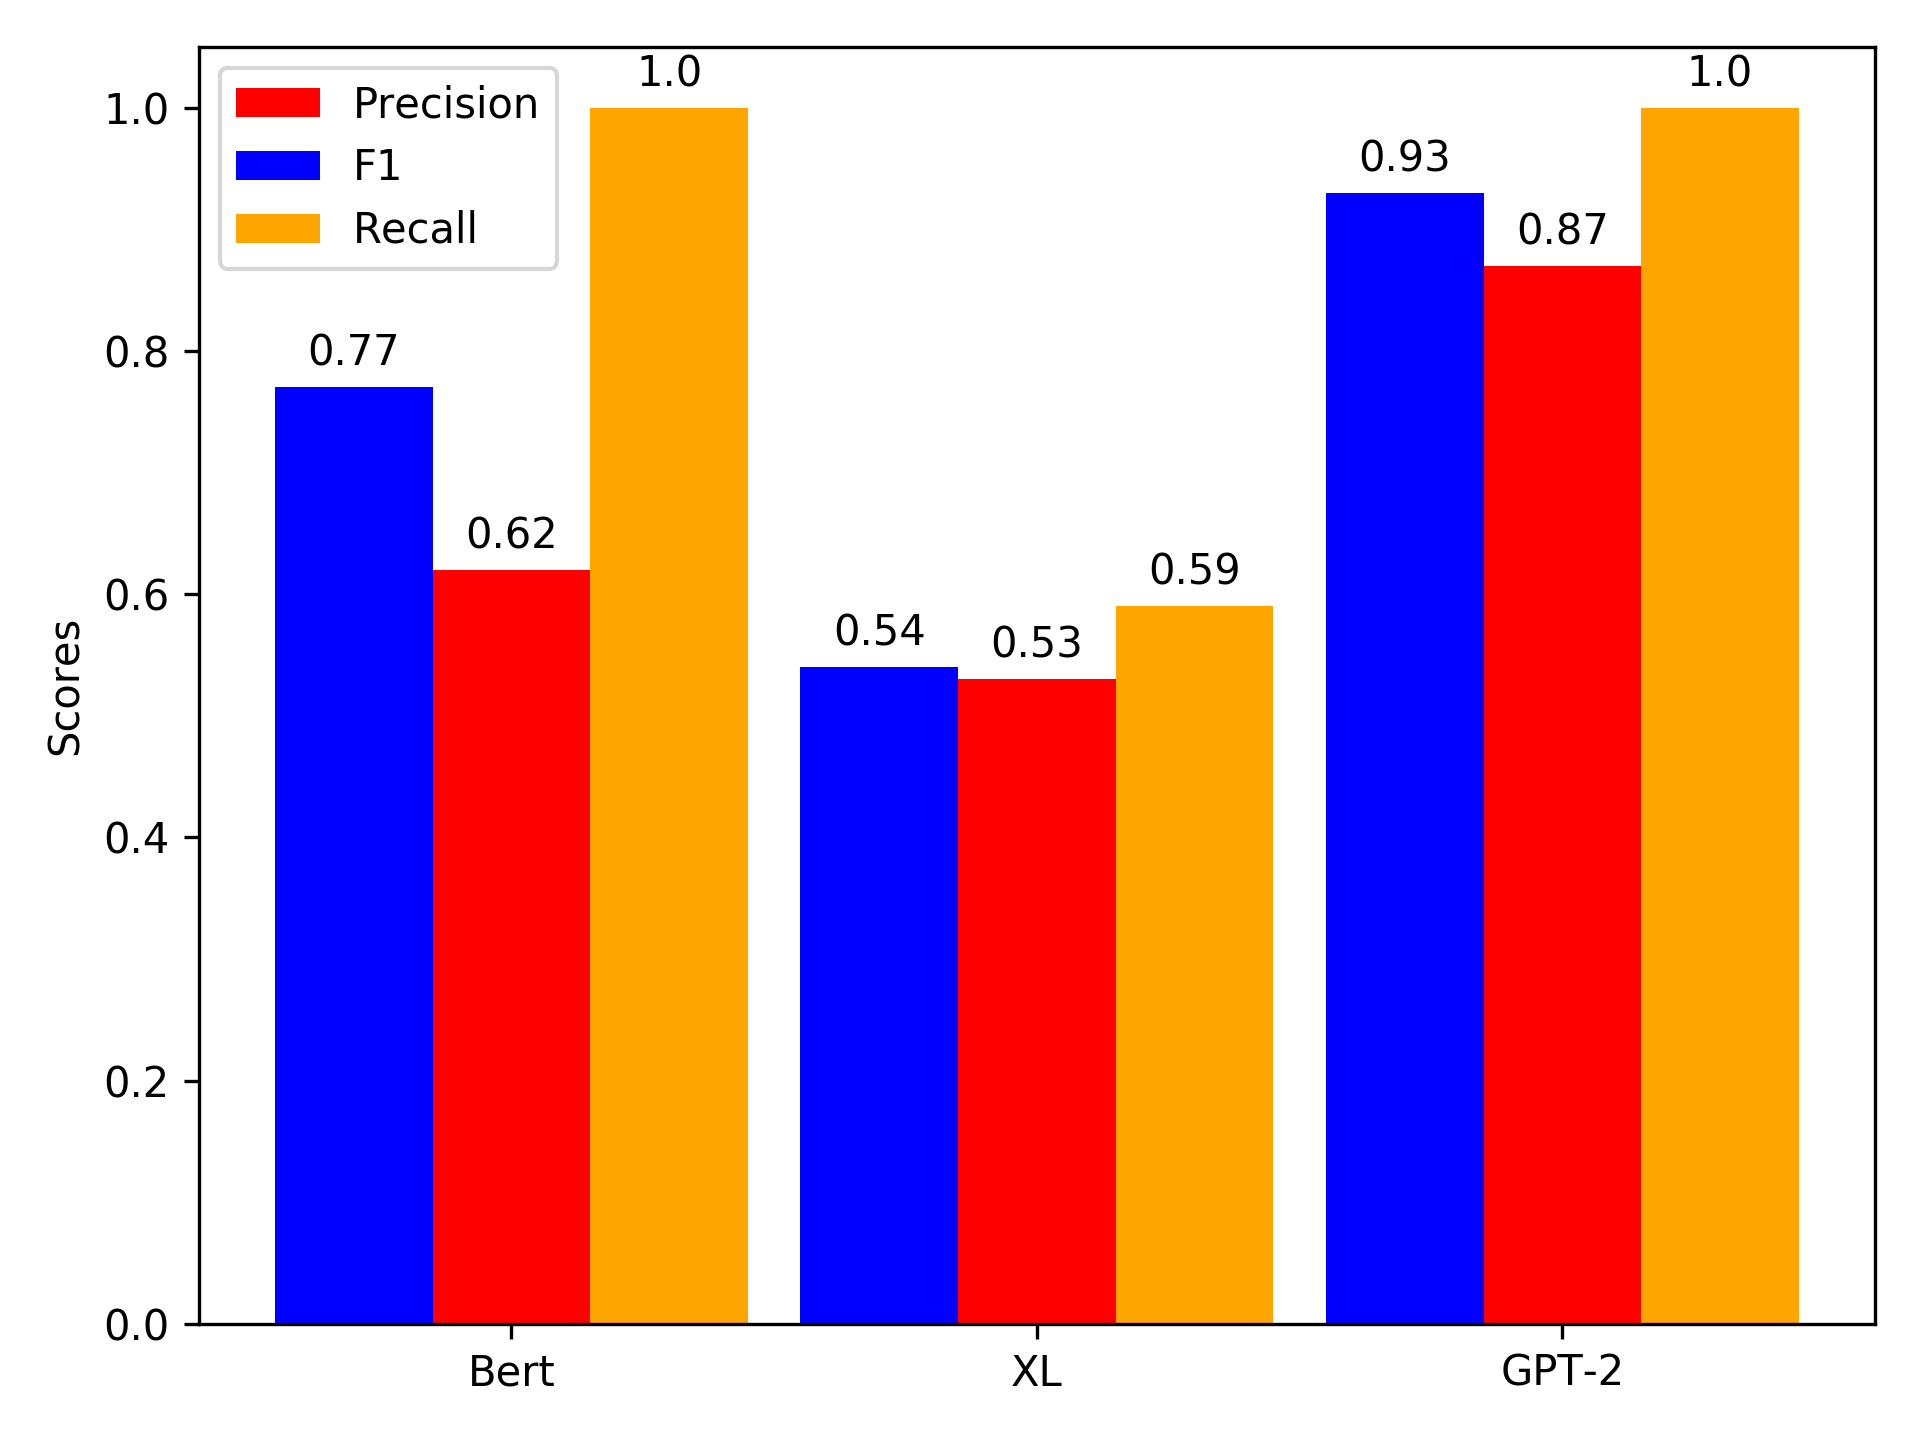
\includegraphics[trim={1cm 0.5cm 0cm 1cm}, width=0.322\textwidth]{results/average/regression_qualitative_average_ratio_0.05.png}}
\hspace{\fill}
   \subfloat[10\% alteration\label{fig:results_regression_qualitative_10} ]{%
      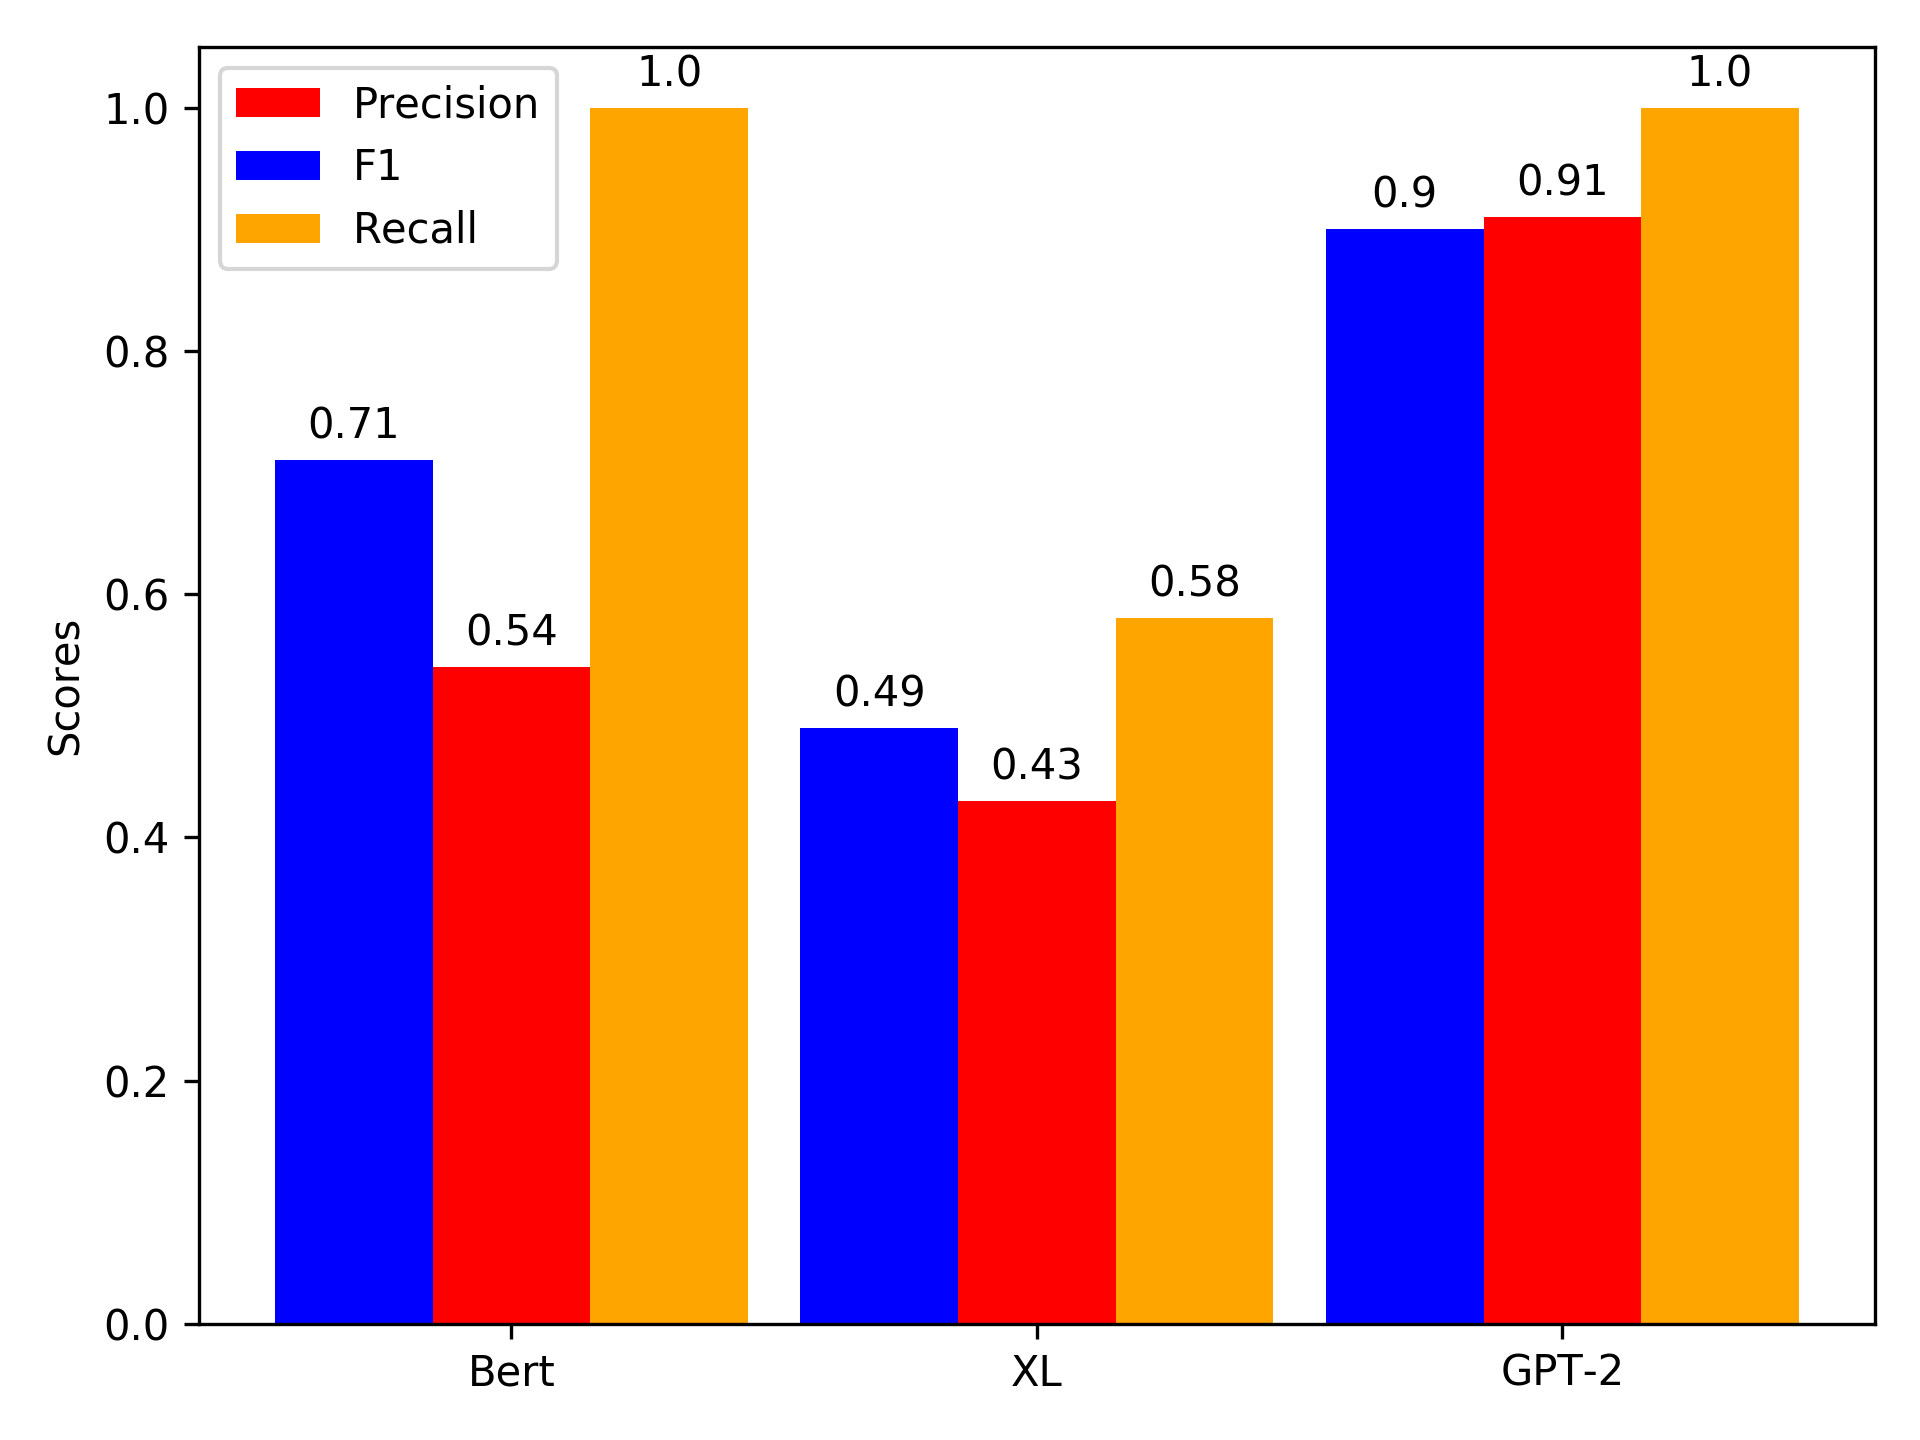
\includegraphics[trim={1cm 0.5cm 0cm 1cm}, width=0.322\textwidth]{results/average/regression_qualitative_average_ratio_0.10.png}}
\hspace{\fill}
   \subfloat[15\% alteration\label{fig:results_regression_qualitative_15}]{%
      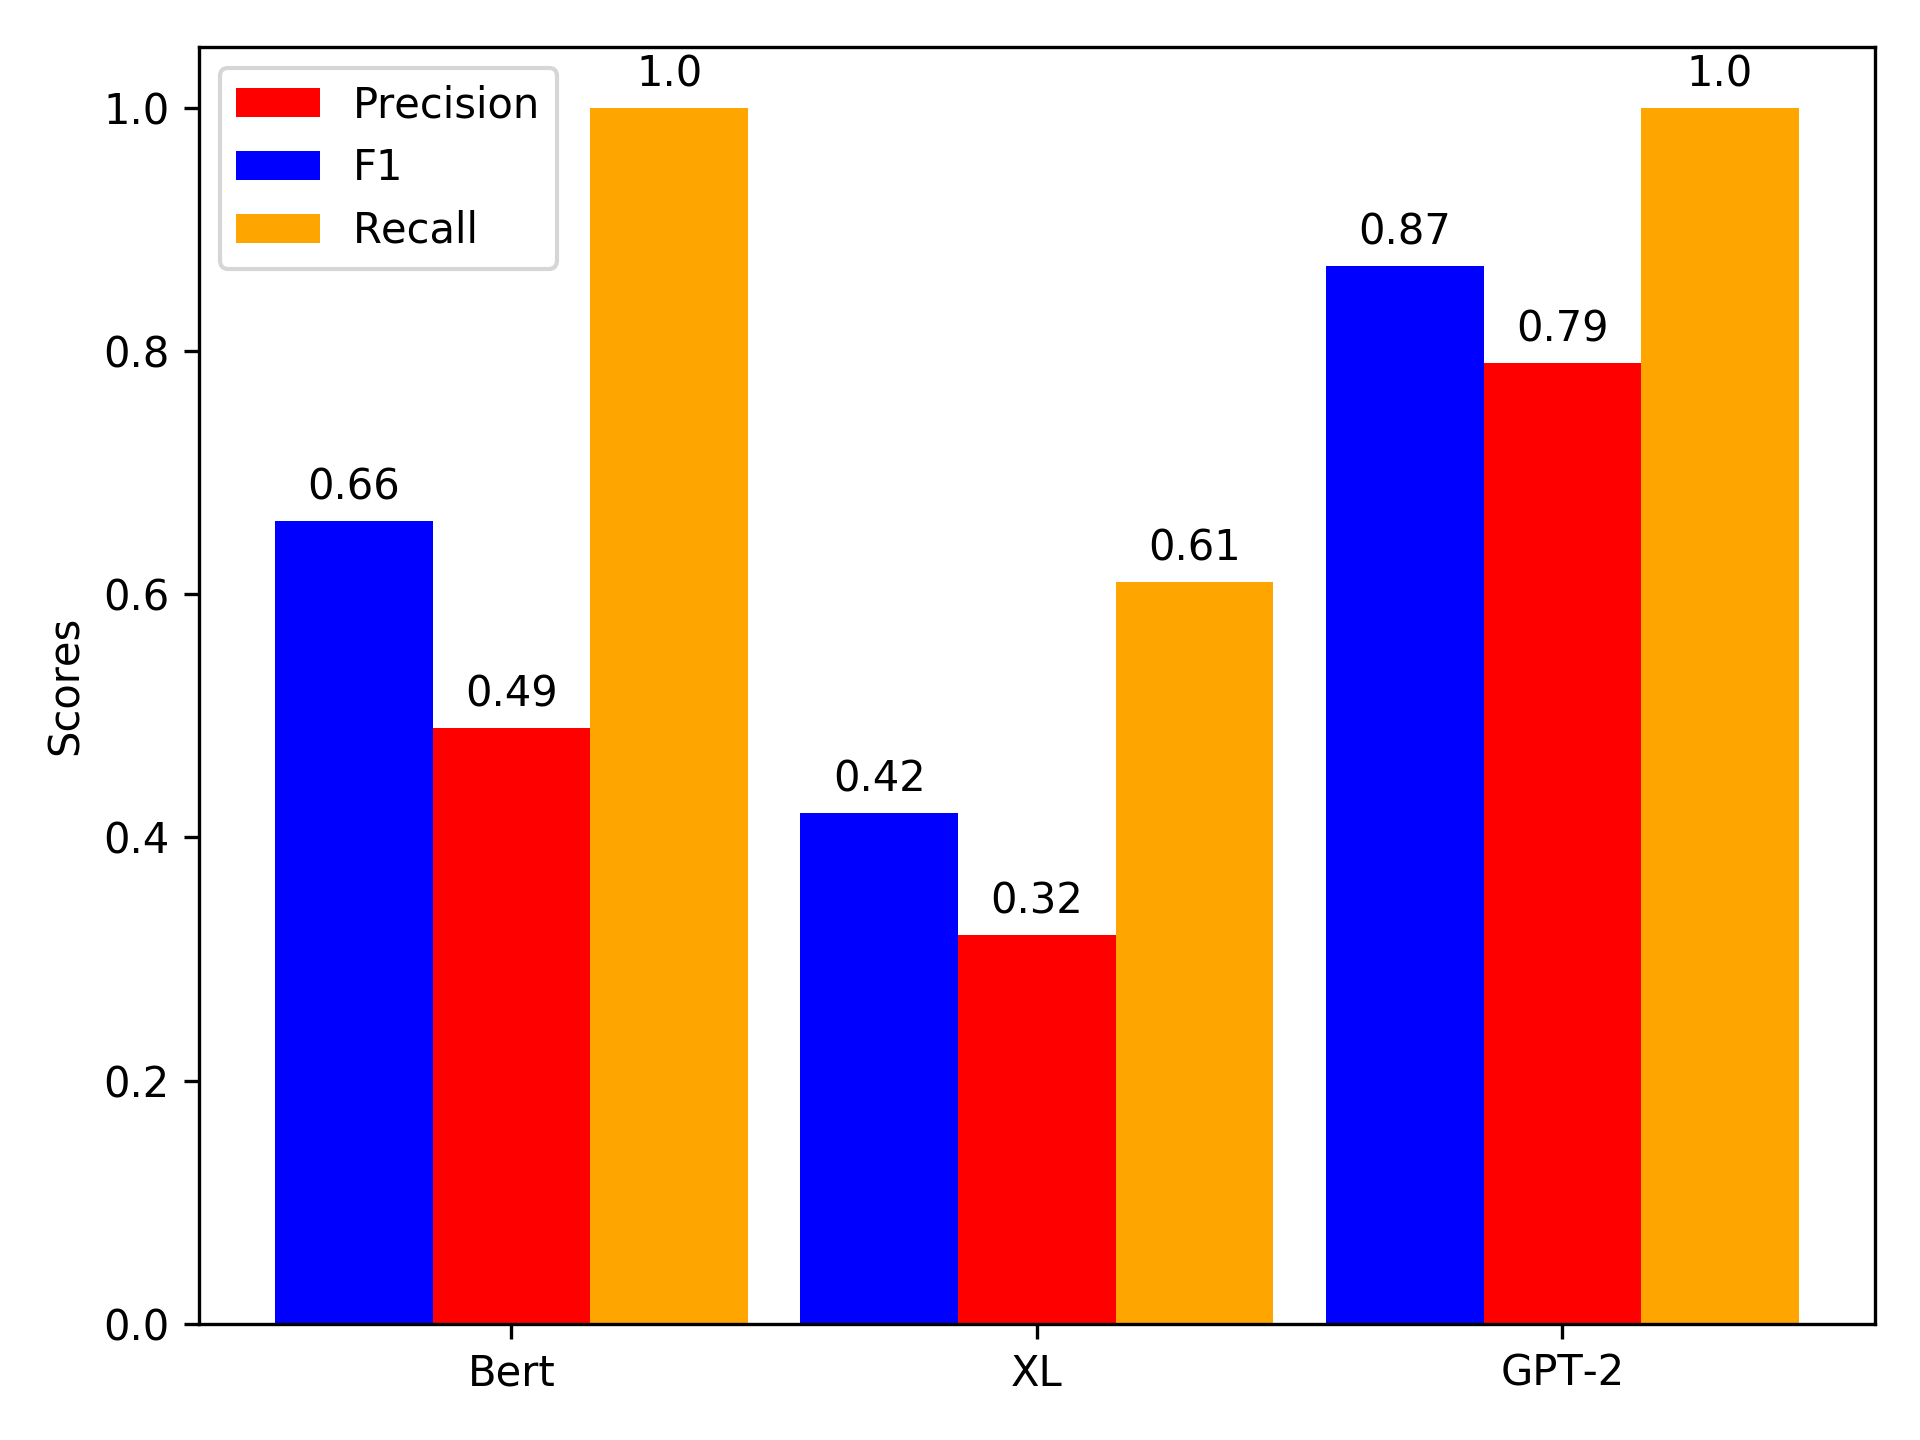
\includegraphics[trim={1cm 0.5cm 0cm 1cm}, width=0.322\textwidth]{results/average/regression_qualitative_average_ratio_0.15.png}}\\
\caption{\label{fig:results_regression_words}Altering log lines at different ratios,  5\% anomalies, using regression.}
\end{figure*}	

%%%%%

\begin{figure}[H]
  \centering
  \captionsetup{justification=centering}
  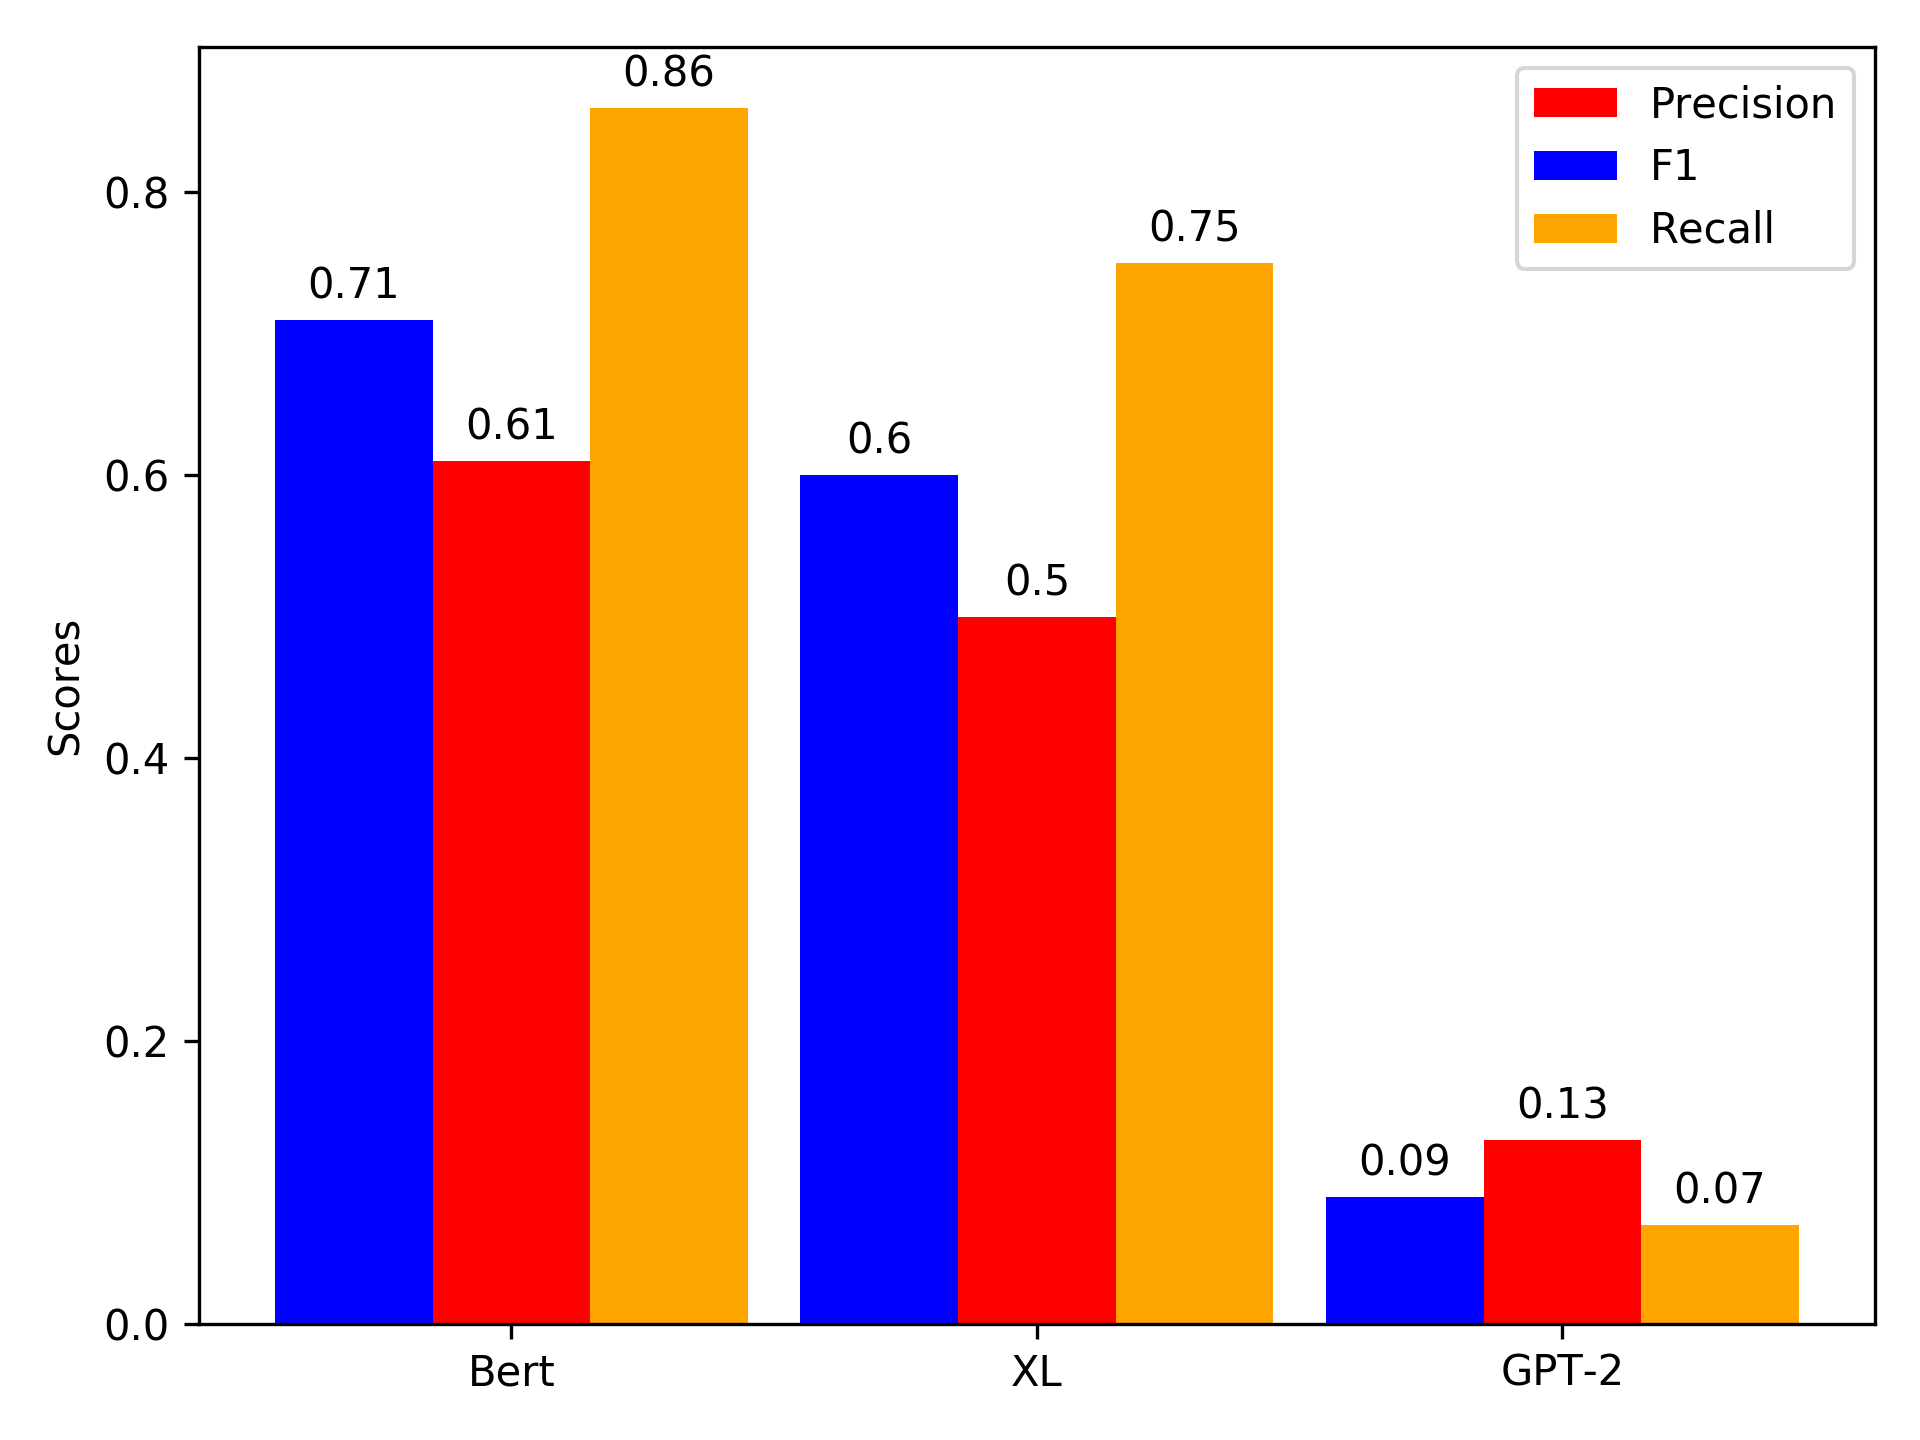
\includegraphics[width=8cm]{results/regression_replace_half.png}\\
  \caption{For 15\% of lines, replace 50\% of words, mark as anomaly, using regression.}
  \label{fig:replace_words_regression}
\end{figure}

\begin{figure}[H]
  \centering
  \captionsetup{justification=centering}
  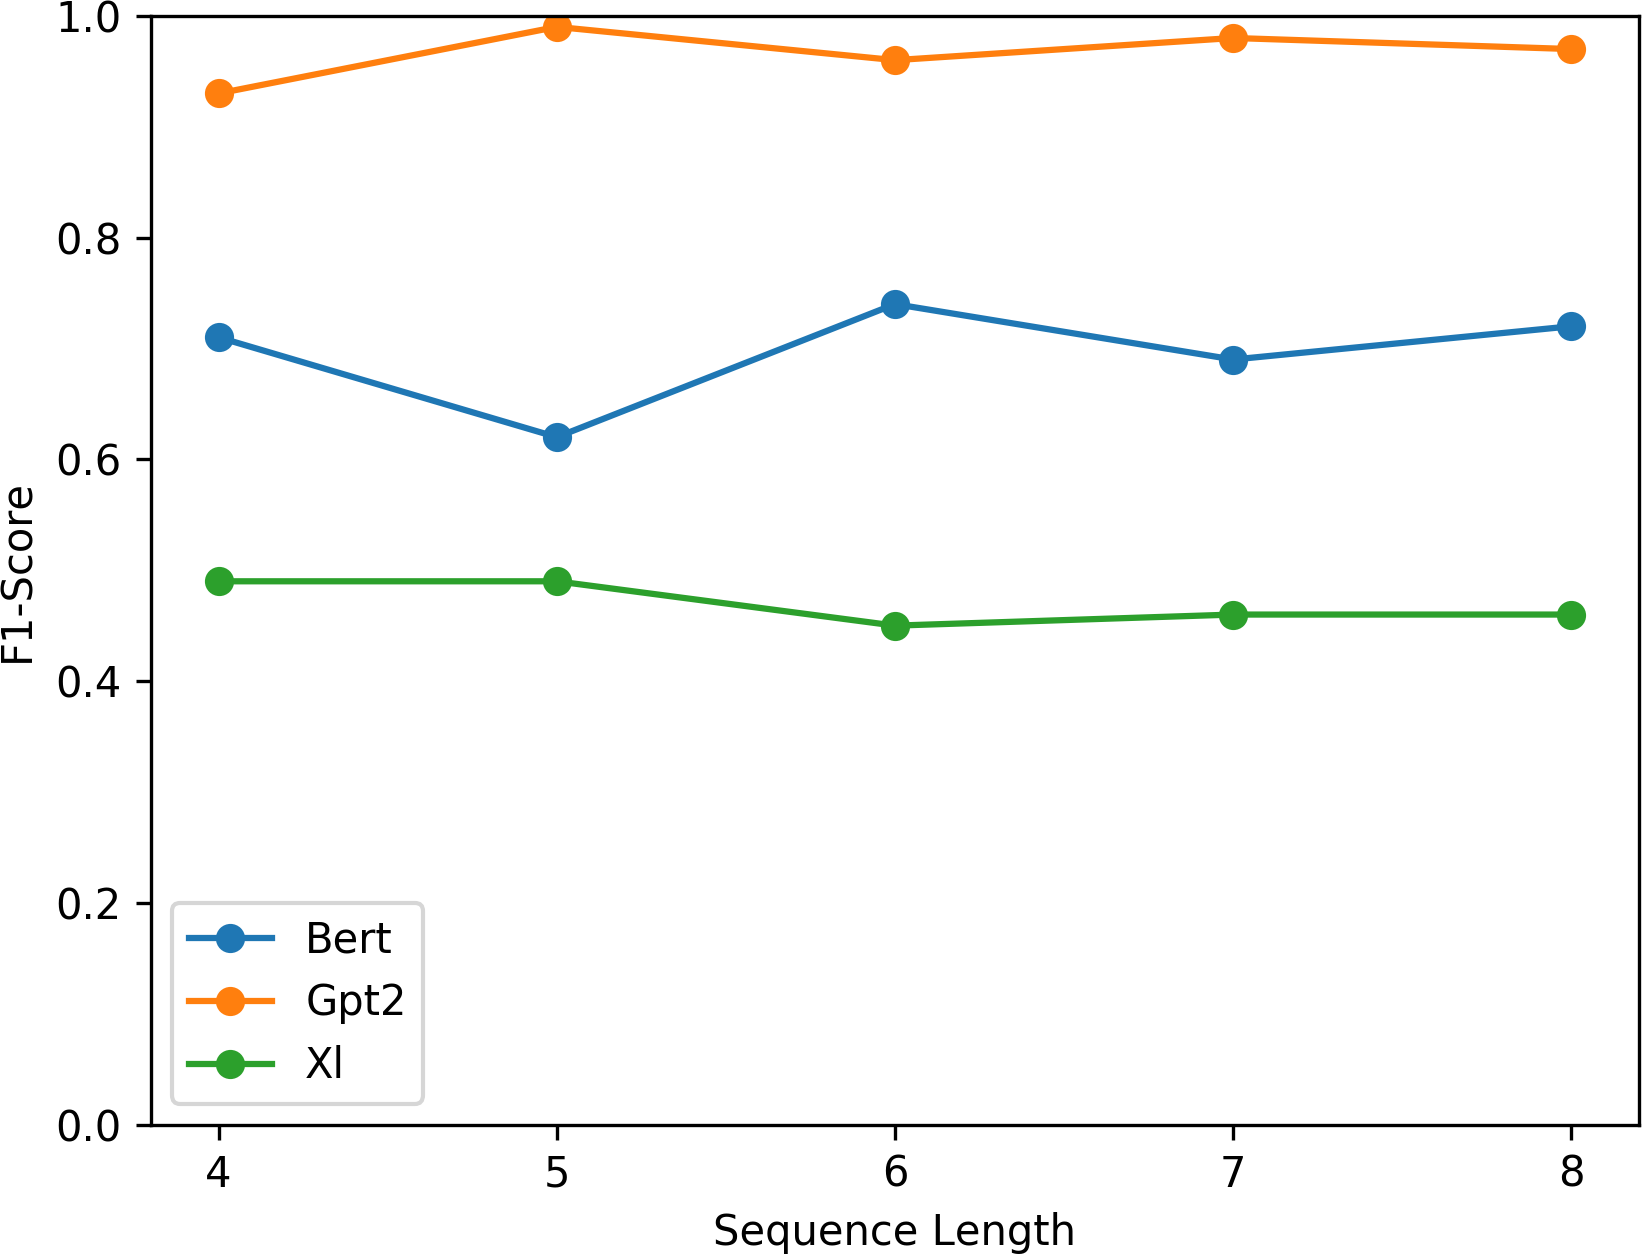
\includegraphics[width=9cm,height=6.5cm]{results/seq_len/sequence_len_regression.png}\\
  \caption{F1-Score for varying input sequence lengths, 15\% word insertion alterations, 5\% anomalies injected, using regression.}
  \label{fig:seq_len_regression}
\end{figure}




\newpage
%%%%%%%%%%%%%%%%
% CLASSIFICATION 
%%%%%%%%%%%%%%%%
\subsection{Classification-based approach using one dataset \label{sec:results-classification}}
In this subsection, the results of the classification-based approach are presented, under the exact same conditions as in \ref{sec:results-regression}. 
The ability of the system to detect injected anomalies, despite alterations on the sequences of logs, i.e. deleting, shuffling and duplicating events, can be seen in \ref{fig:results_multiclass_sequential}. For the classification-based approach we can see a different picture than for the regression-based approach, where GPT-2 showed better results. For classification though, Bert and XL-Transformers show recall values of 1.0 throughout, where GPT-2 only reaches recall values of around 0.7. Bert reaches F1-scores of 0.67 for 5\% alterations, 0.59 for 10\% alterations and 0.54 for 15\% alterations, while XL-Transformers goes from 0.51 for 5\% to 0.41 for 15\% alterations and GPT-2 from 0.44 for 5\% alterations to 0.36 for 15\% alterations. For precision, Bert reaches 0.37 for 15\% alterations, XL-Transformers 0.25 and GPT-2 0.24.
Bert shows the best F1-score and precision throughout, while GPT-2 comes in last for every metric. While Bert clearly takes the first place overall, it is followed by XL-Transformers and GPT-2.

The impact of alterations on the logs themselves, i.e. inserting, removing and replacing words are summarised in figure \ref{fig:results_multiclass_qualitative}. Again, only average results on the individual injections are presented. Results broken down by each alteration can be found in the appendix \ref{appendix:classification}.
Here it is again evident, similarly to the results for the regression-based approach, that both Bert and XL-Transformers perform better for the alterations on the logs themselves than alterations on the sequence of logs, while GPT-2 performs slightly worse. Again, as for the alterations on the log sequences, Bert and XL-Transformers both reach a recall value of 1.0, while GPT-2 reaches a recall value of around 0.7 for all alteration ratios. Bert shows a good F1-score of 0.77 for 5\% alterations, 0.7 for 10\% alterations and 0.67 for 15 \% alterations. XL-Transformers reaches a F1-score of 0.58 for 5\% alterations, 0.55 for 10\% alterations and 0.53 for 15\% alterations. GPT-2 shows F1-scores of 0.53 for 5\% alterations, 0.46 for 10\% alterations, and 0.43 for 15\% alterations. For precision, Bert shows the best results, followed by XL-Transformers and GPT-2.

In contrary to the results using regression, the classification approach seems most fit for Bert and much less for GPT-2. This is probably due to the smaller cosine distance between the templates in GPT-2, which makes it harder for the system to correctly assign the templates to the classes in the prediction process.

The impact of the input sequence length can be seen in \ref{fig:seq_len_regression}. Bert again seems to profit slightly from sequence lengths longer than 6 or 7, whereas the quality of results for XL-Transformers and GPT-2 seem to have a tendency to degrade in prediction quality for longer input sequence lengths.


%\begin{figure}[h]
%  \centering
%  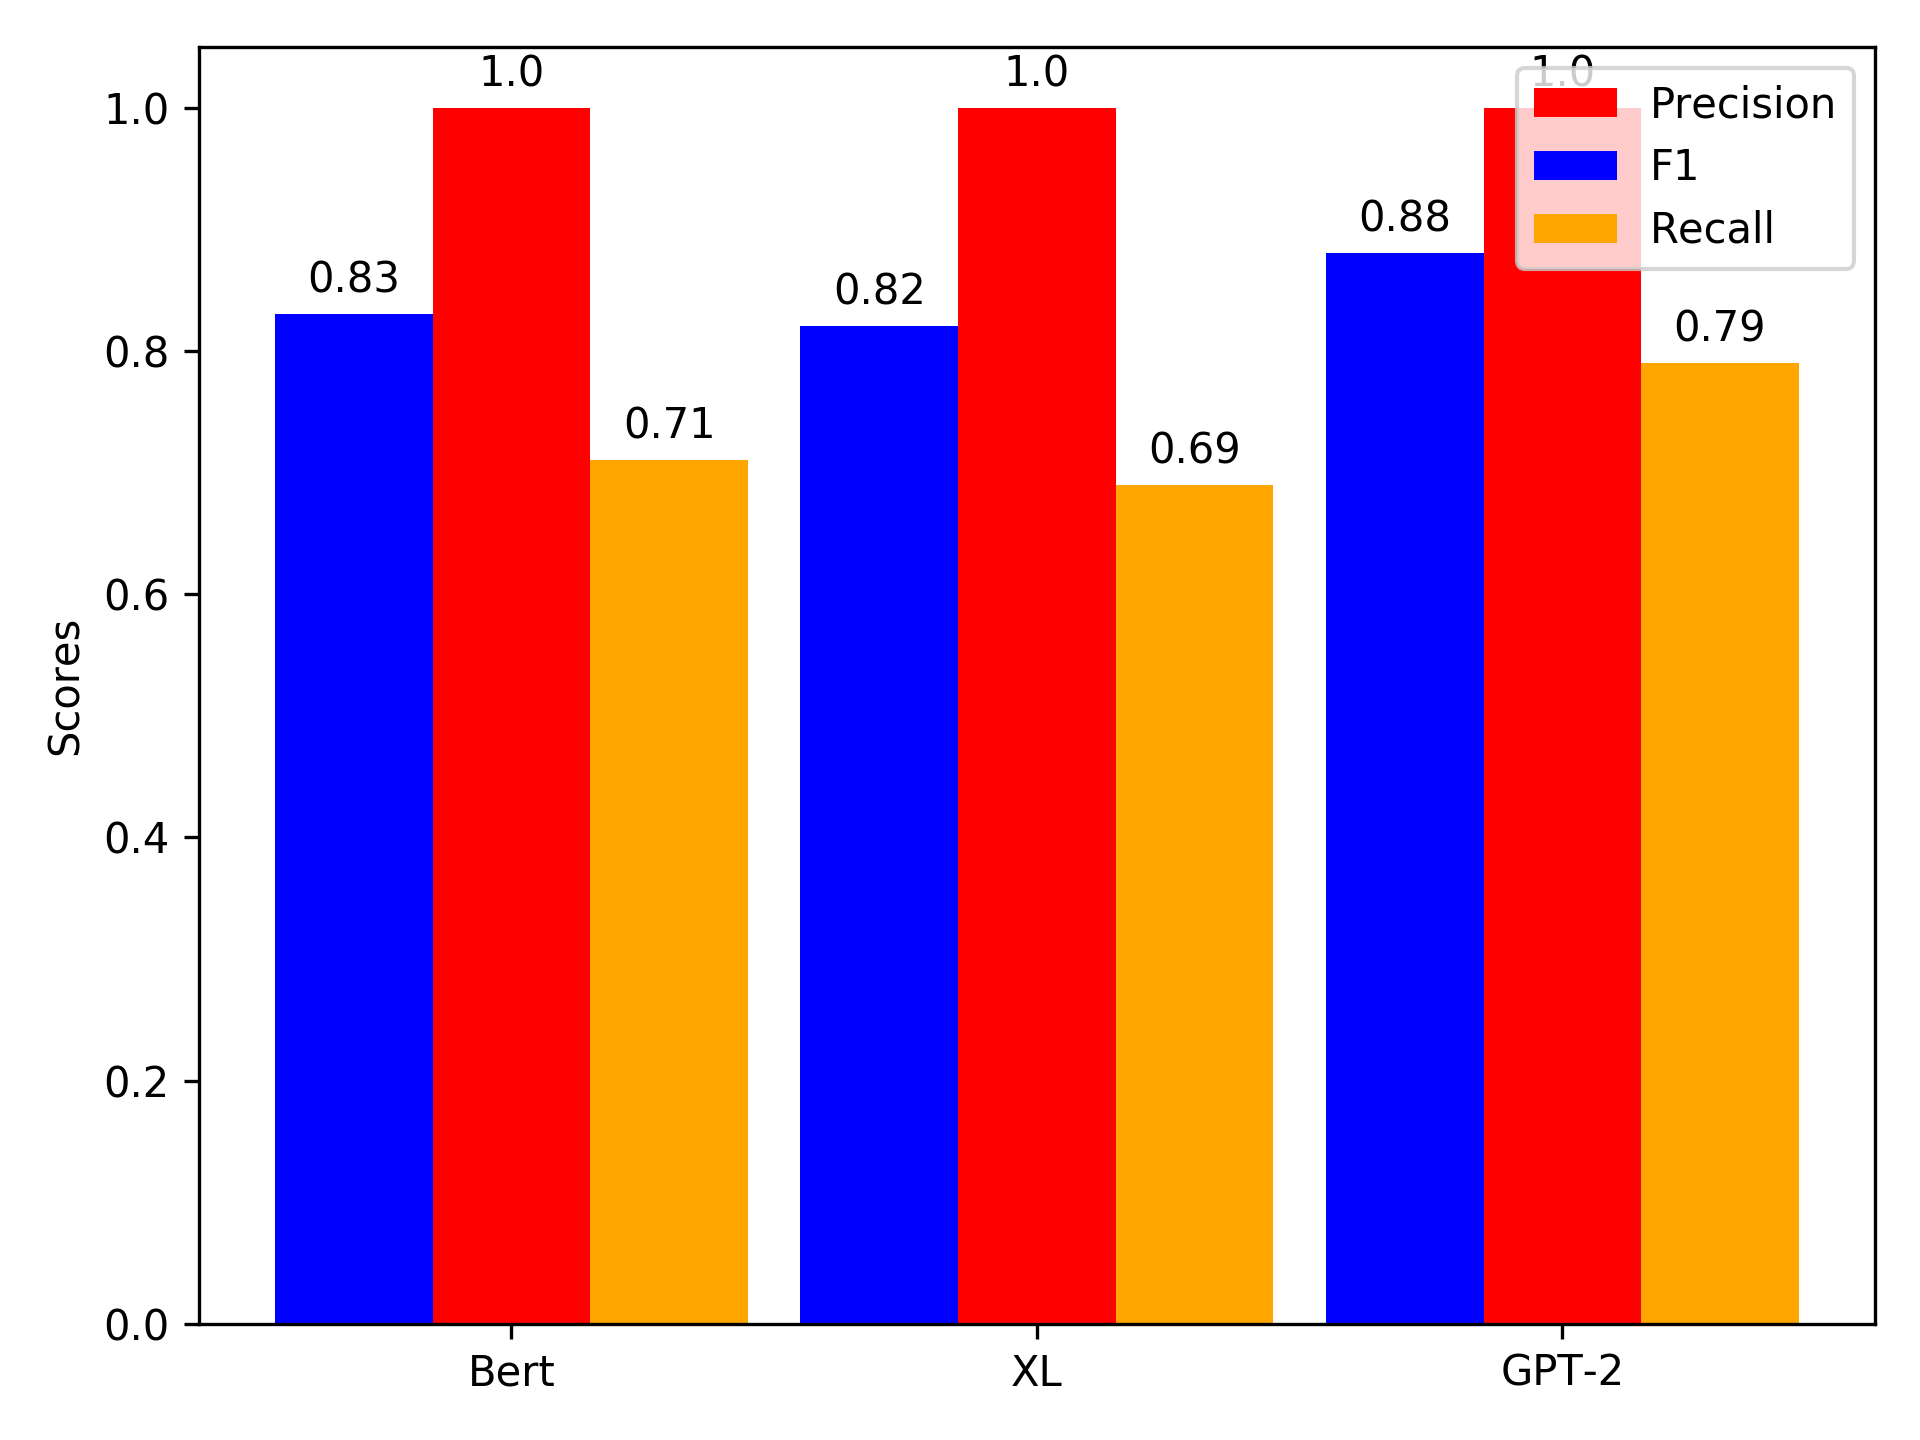
\includegraphics[width=6cm,height=4.5cm]{results/classification_sequence/multiclass_reverse.png}\\
%  \caption{Scores for detecting reversed order of log events, using classification.}
%  \label{fig:multiclass_reverse_order}
%\end{figure}
% multiclass sequential
\begin{figure*}[ht!]
  \centering
  \captionsetup{justification=centering}
   \subfloat[5\% alteration\label{fig:results_multiclass_sequential_5}]{%
      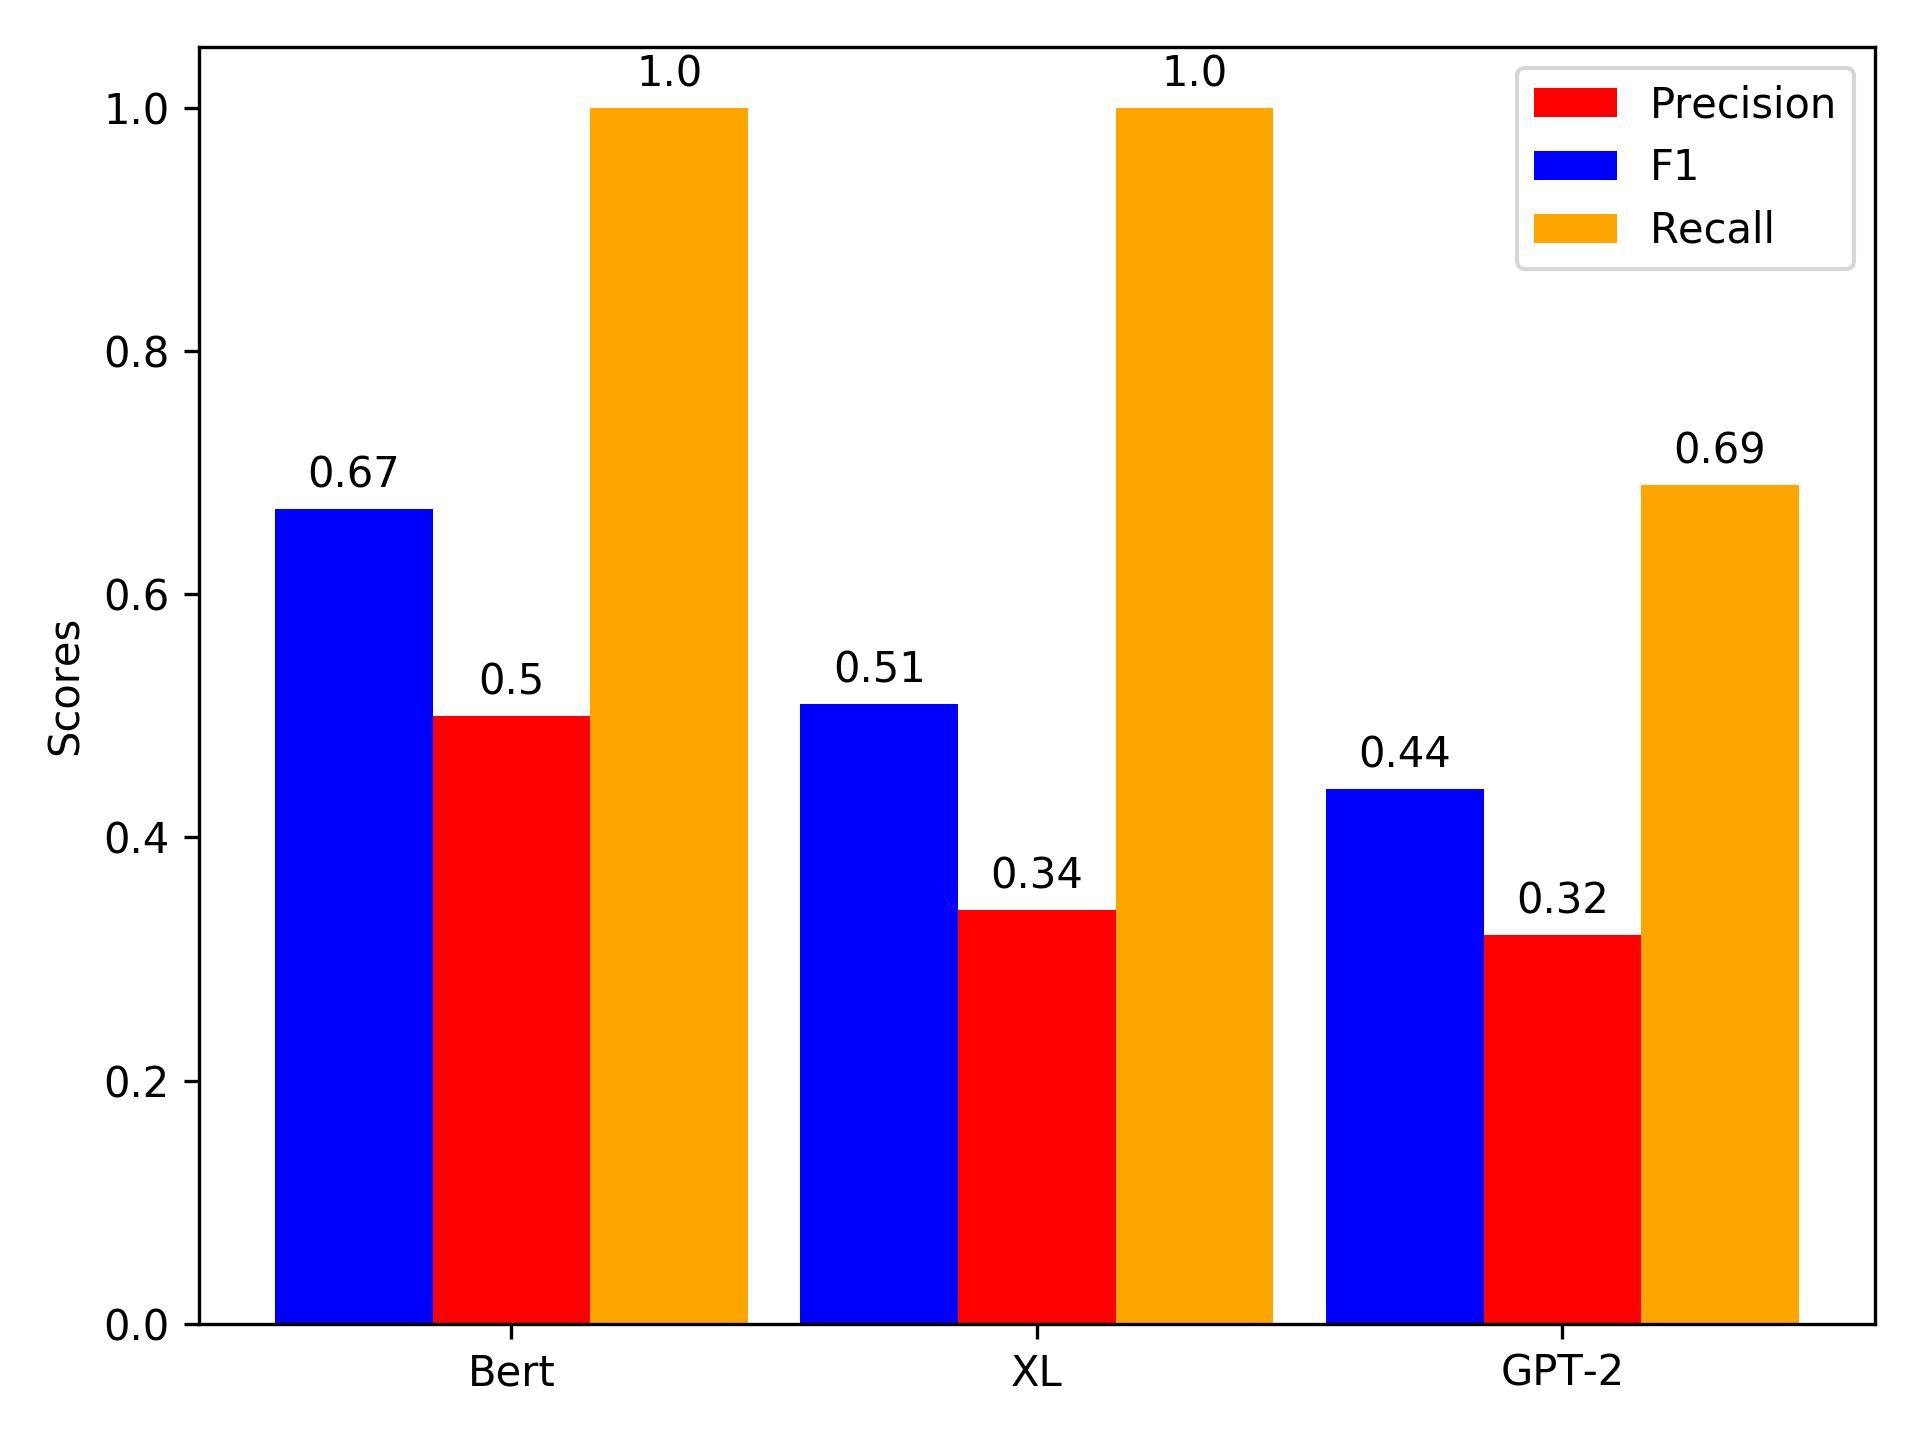
\includegraphics[trim={1cm 0.5cm 0cm 1cm}, width=0.322\textwidth]{results/average/multiclass_sequential_average_ratio_0.05.png}}
\hspace{\fill}
   \subfloat[10\% alteration\label{fig:results_multiclass_sequential_10} ]{%
      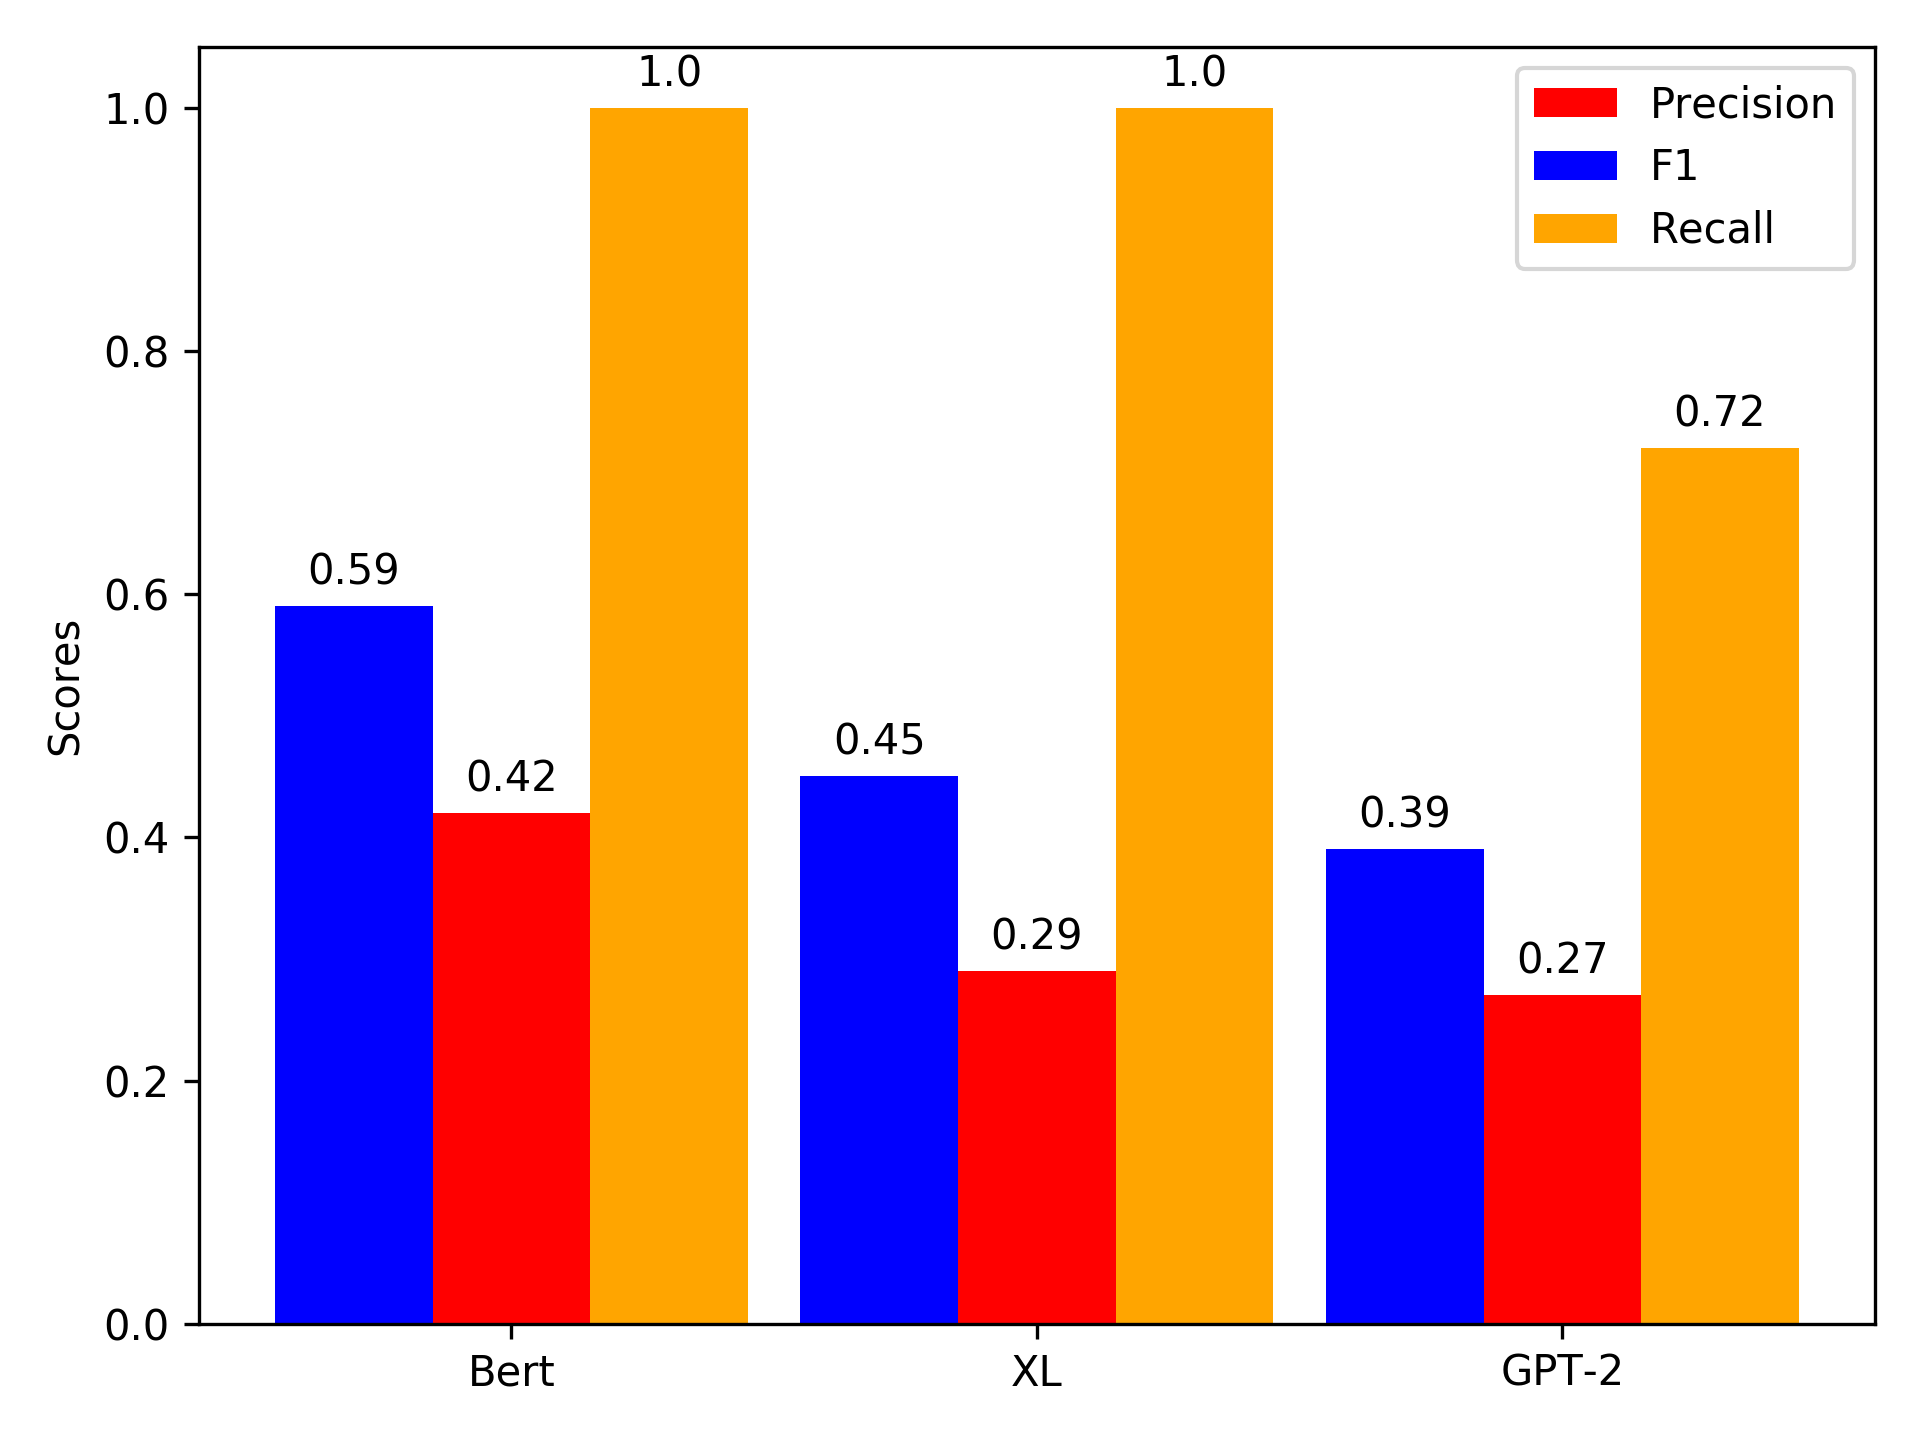
\includegraphics[trim={1cm 0.5cm 0cm 1cm}, width=0.322\textwidth]{results/average/multiclass_sequential_average_ratio_0.10.png}}
\hspace{\fill}
   \subfloat[15\% alteration\label{fig:results_multiclass_sequential_15}]{%
      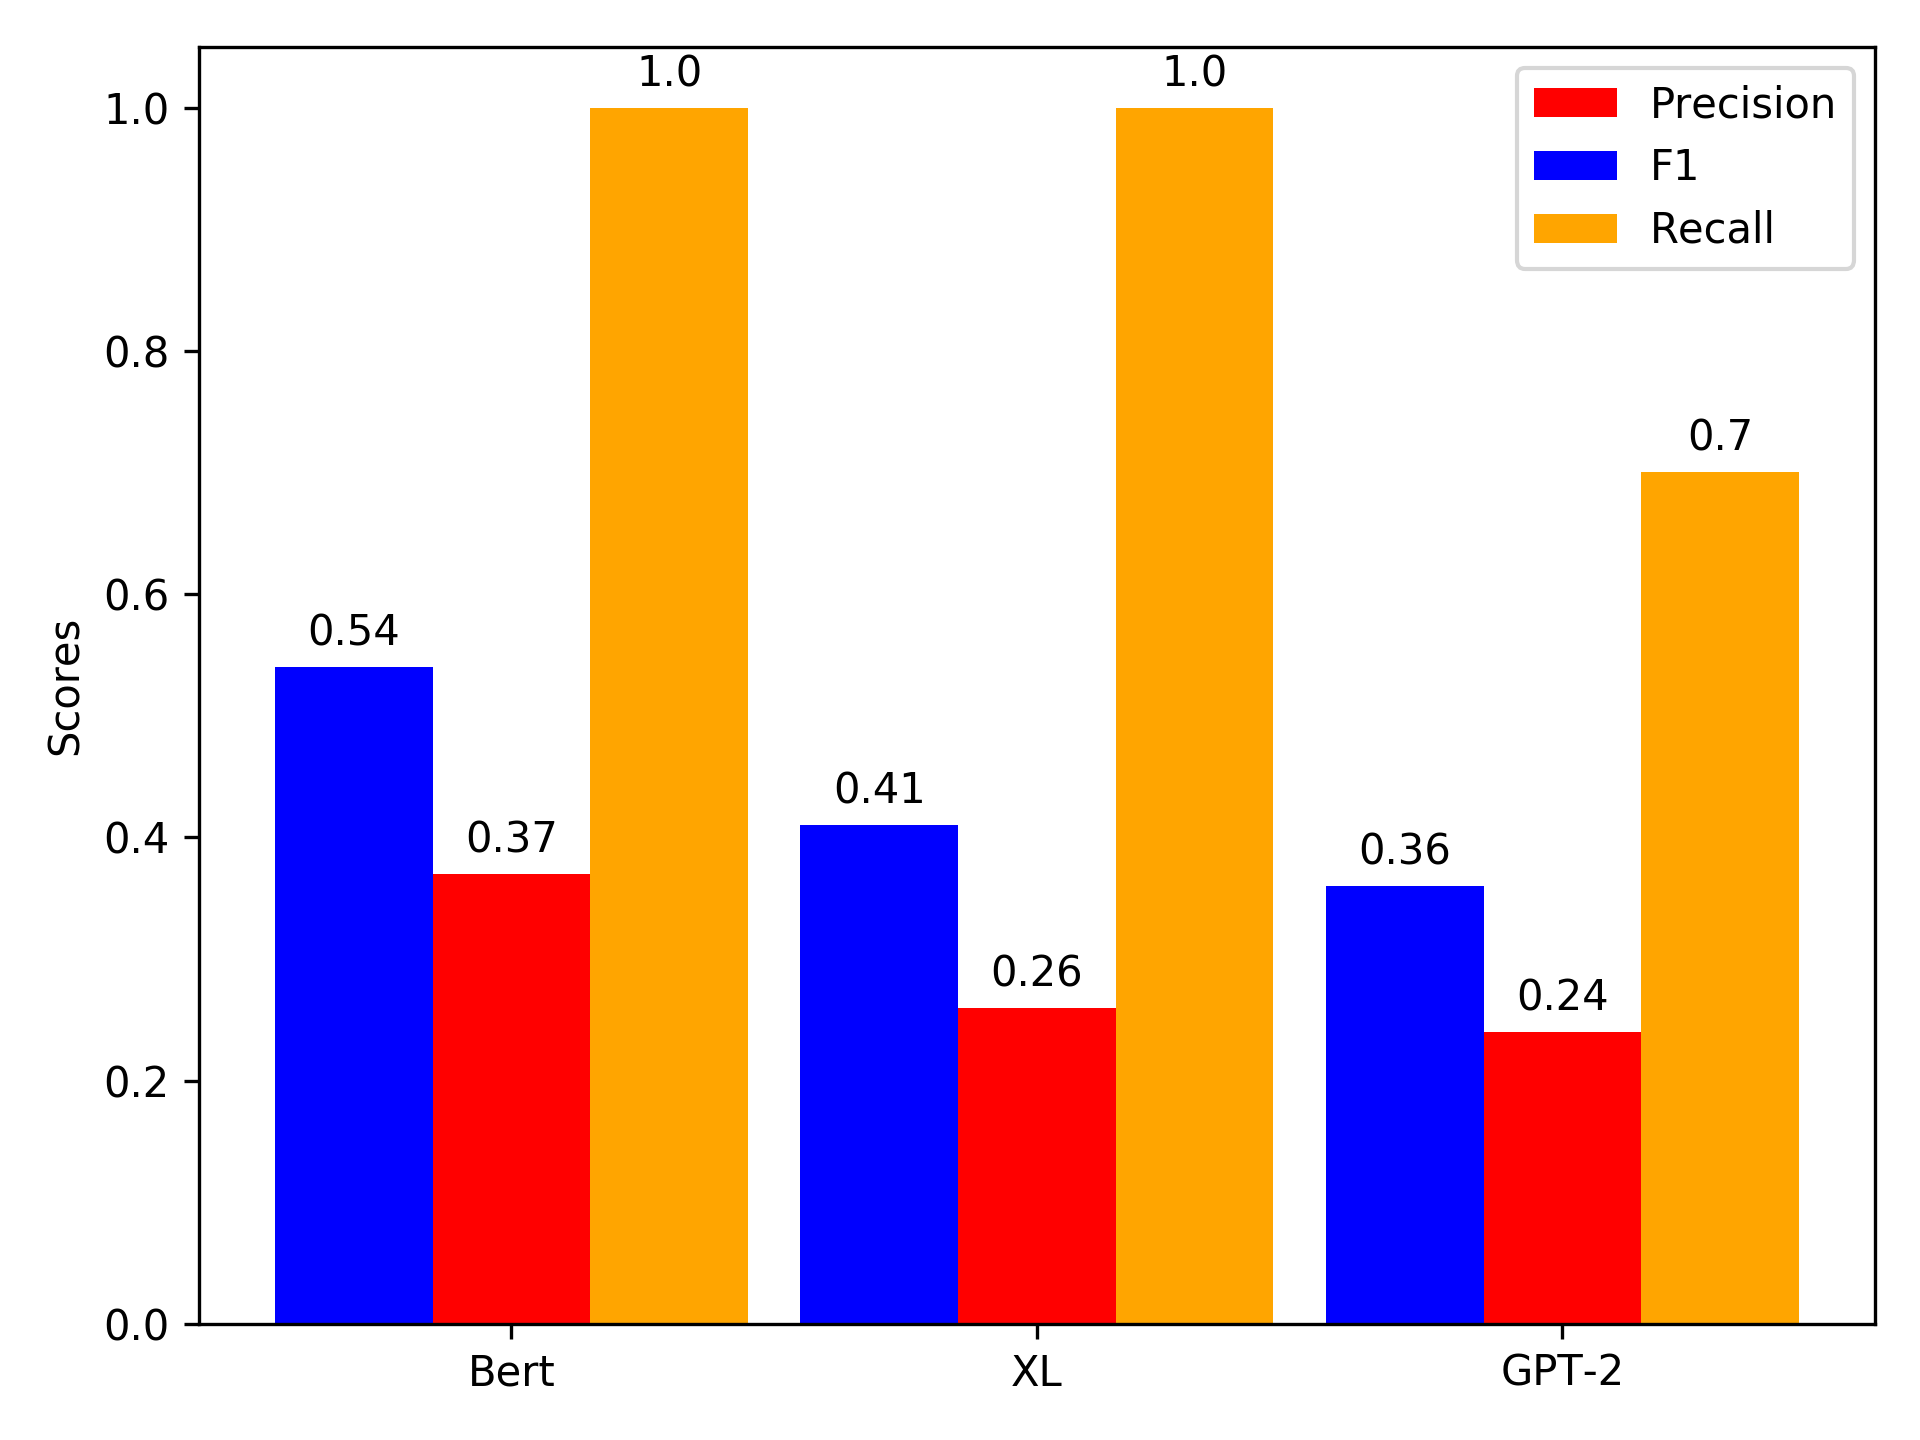
\includegraphics[trim={1cm 0.5cm 0cm 1cm}, width=0.322\textwidth]{results/average/multiclass_sequential_average_ratio_0.15.png}}\\
\caption{\label{fig:results_multiclass_sequential}Altering the order of log sequences at different ratios, 5\% anomalies, using classification.}
\end{figure*}

%multiclass qualitative
\begin{figure*}[ht!]
  \centering
  \captionsetup{justification=centering}
   \subfloat[5\% alteration\label{fig:results_multiclass_qualitative_5}]{%
      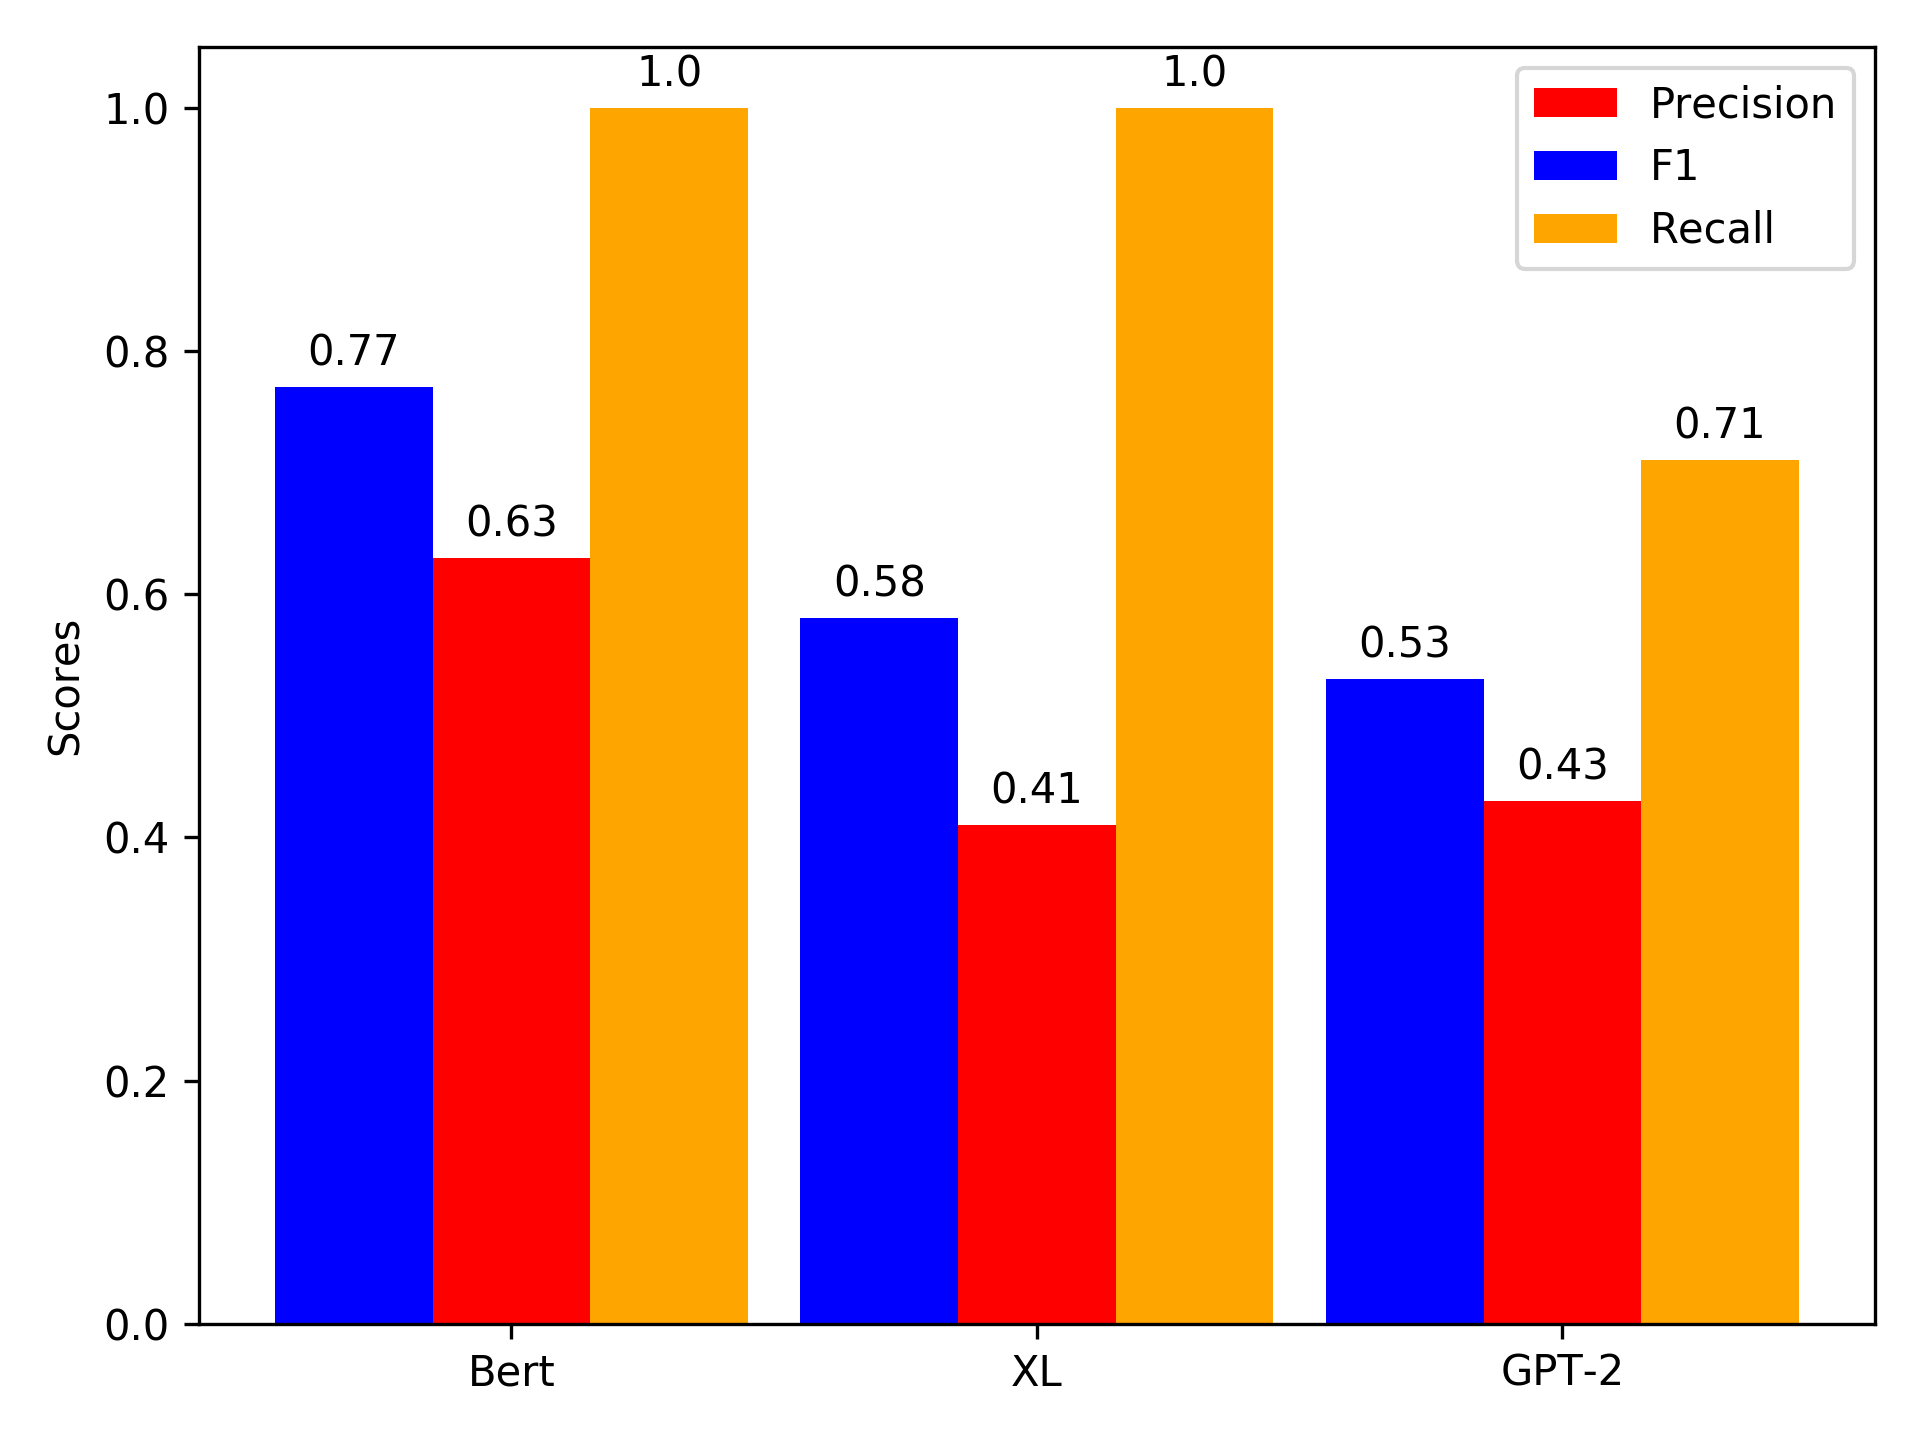
\includegraphics[trim={1cm 0.5cm 0cm 1cm}, width=0.322\textwidth]{results/average/multiclass_qualitative_average_ratio_0.05.png}}
\hspace{\fill}
   \subfloat[10\% alteration\label{fig:results_multiclass_qualitative_10} ]{%
      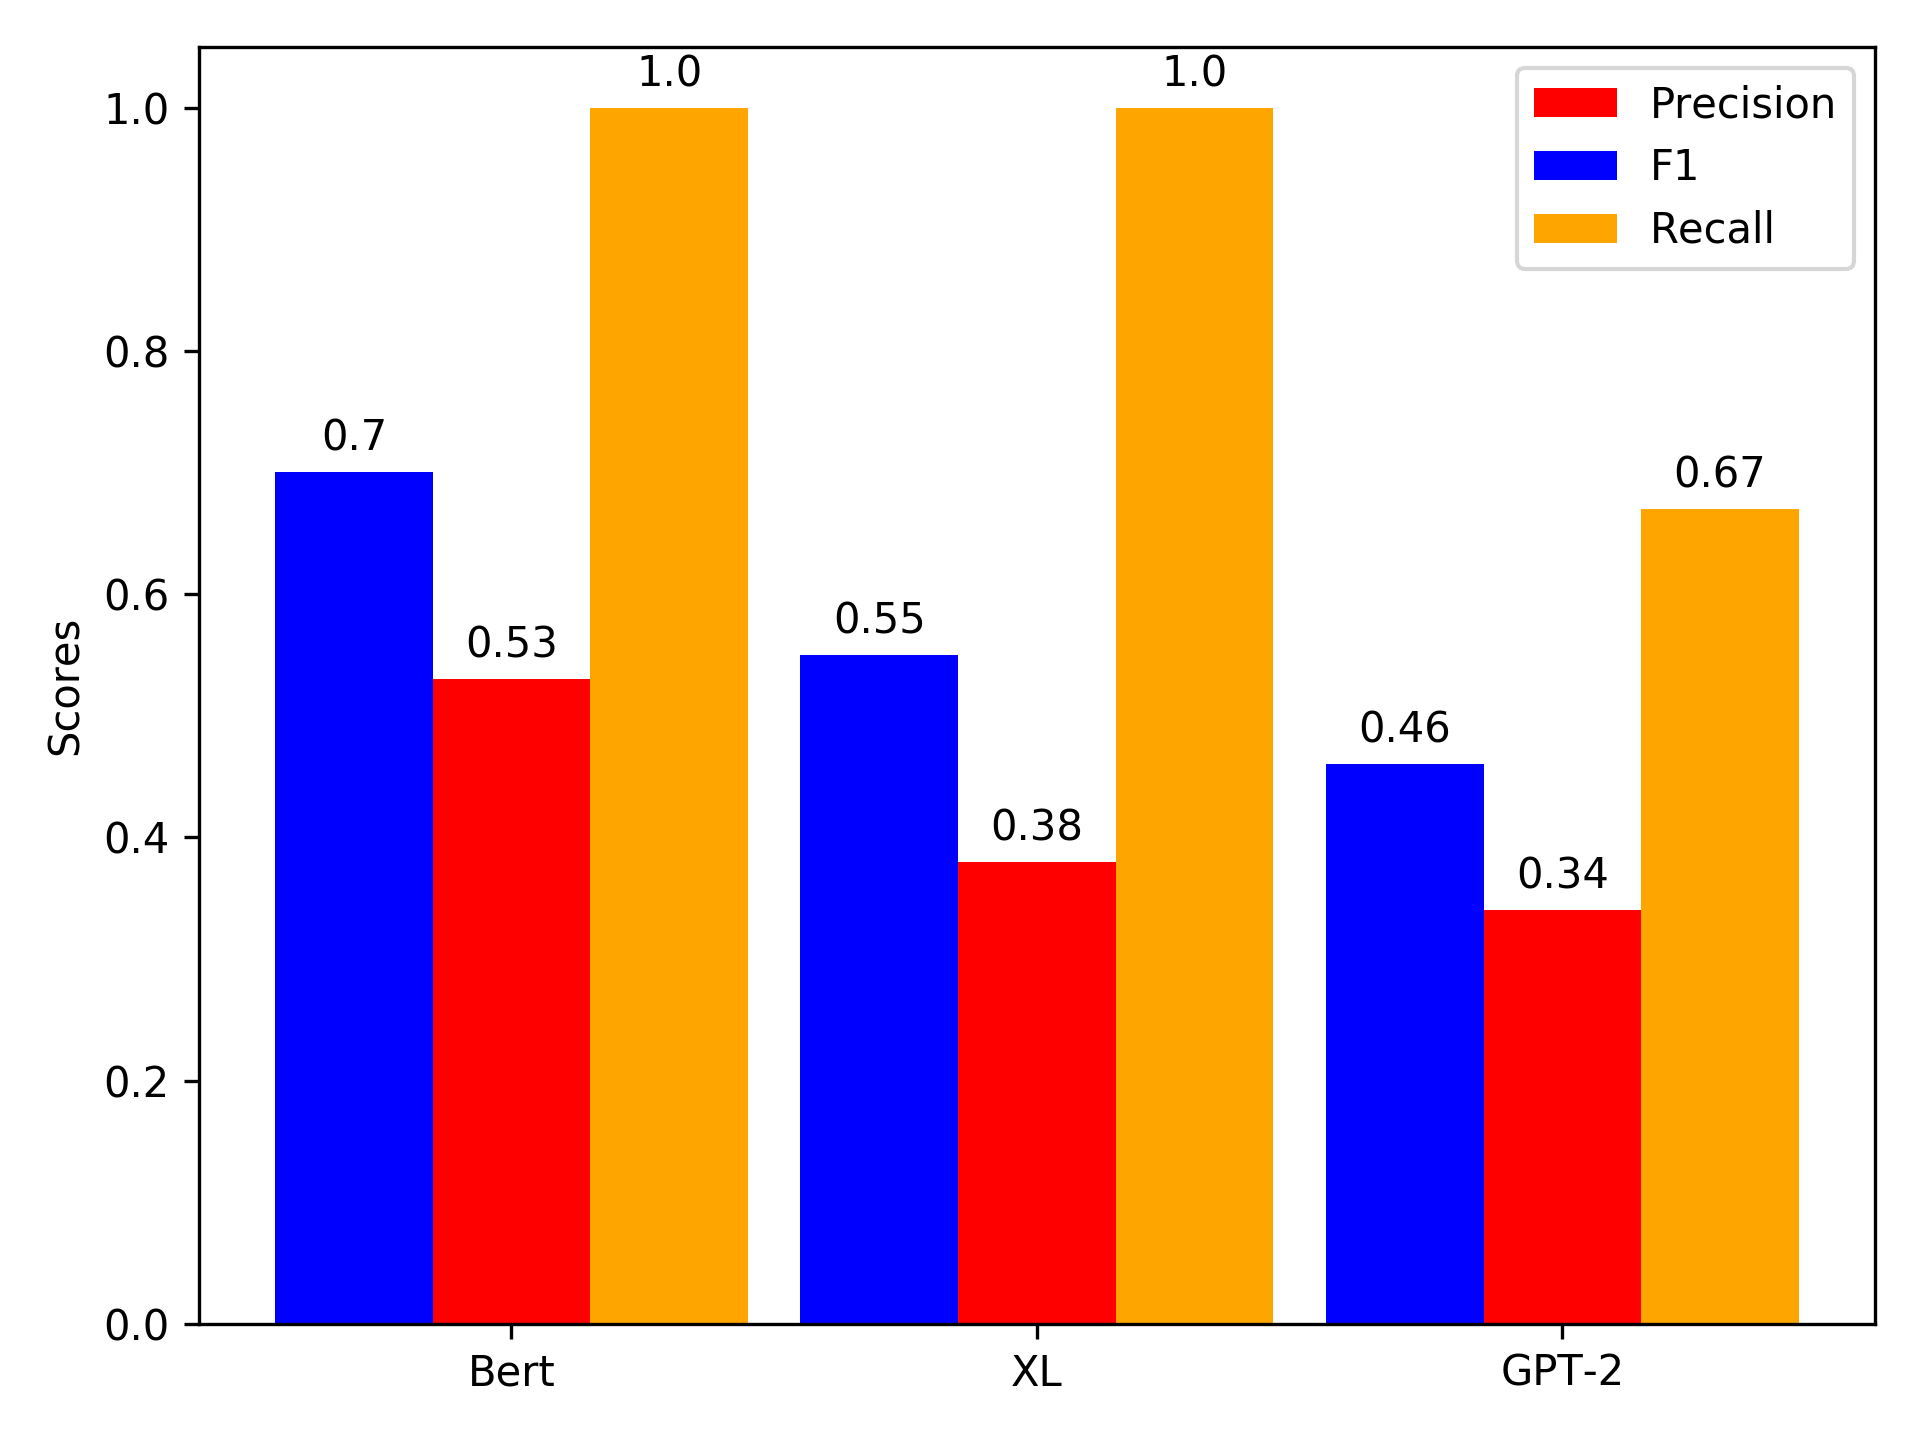
\includegraphics[trim={1cm 0.5cm 0cm 1cm}, width=0.322\textwidth]{results/average/multiclass_qualitative_average_ratio_0.10.png}}
\hspace{\fill}
   \subfloat[15\% alteration\label{fig:results_multiclass_qualitative_15}]{%
      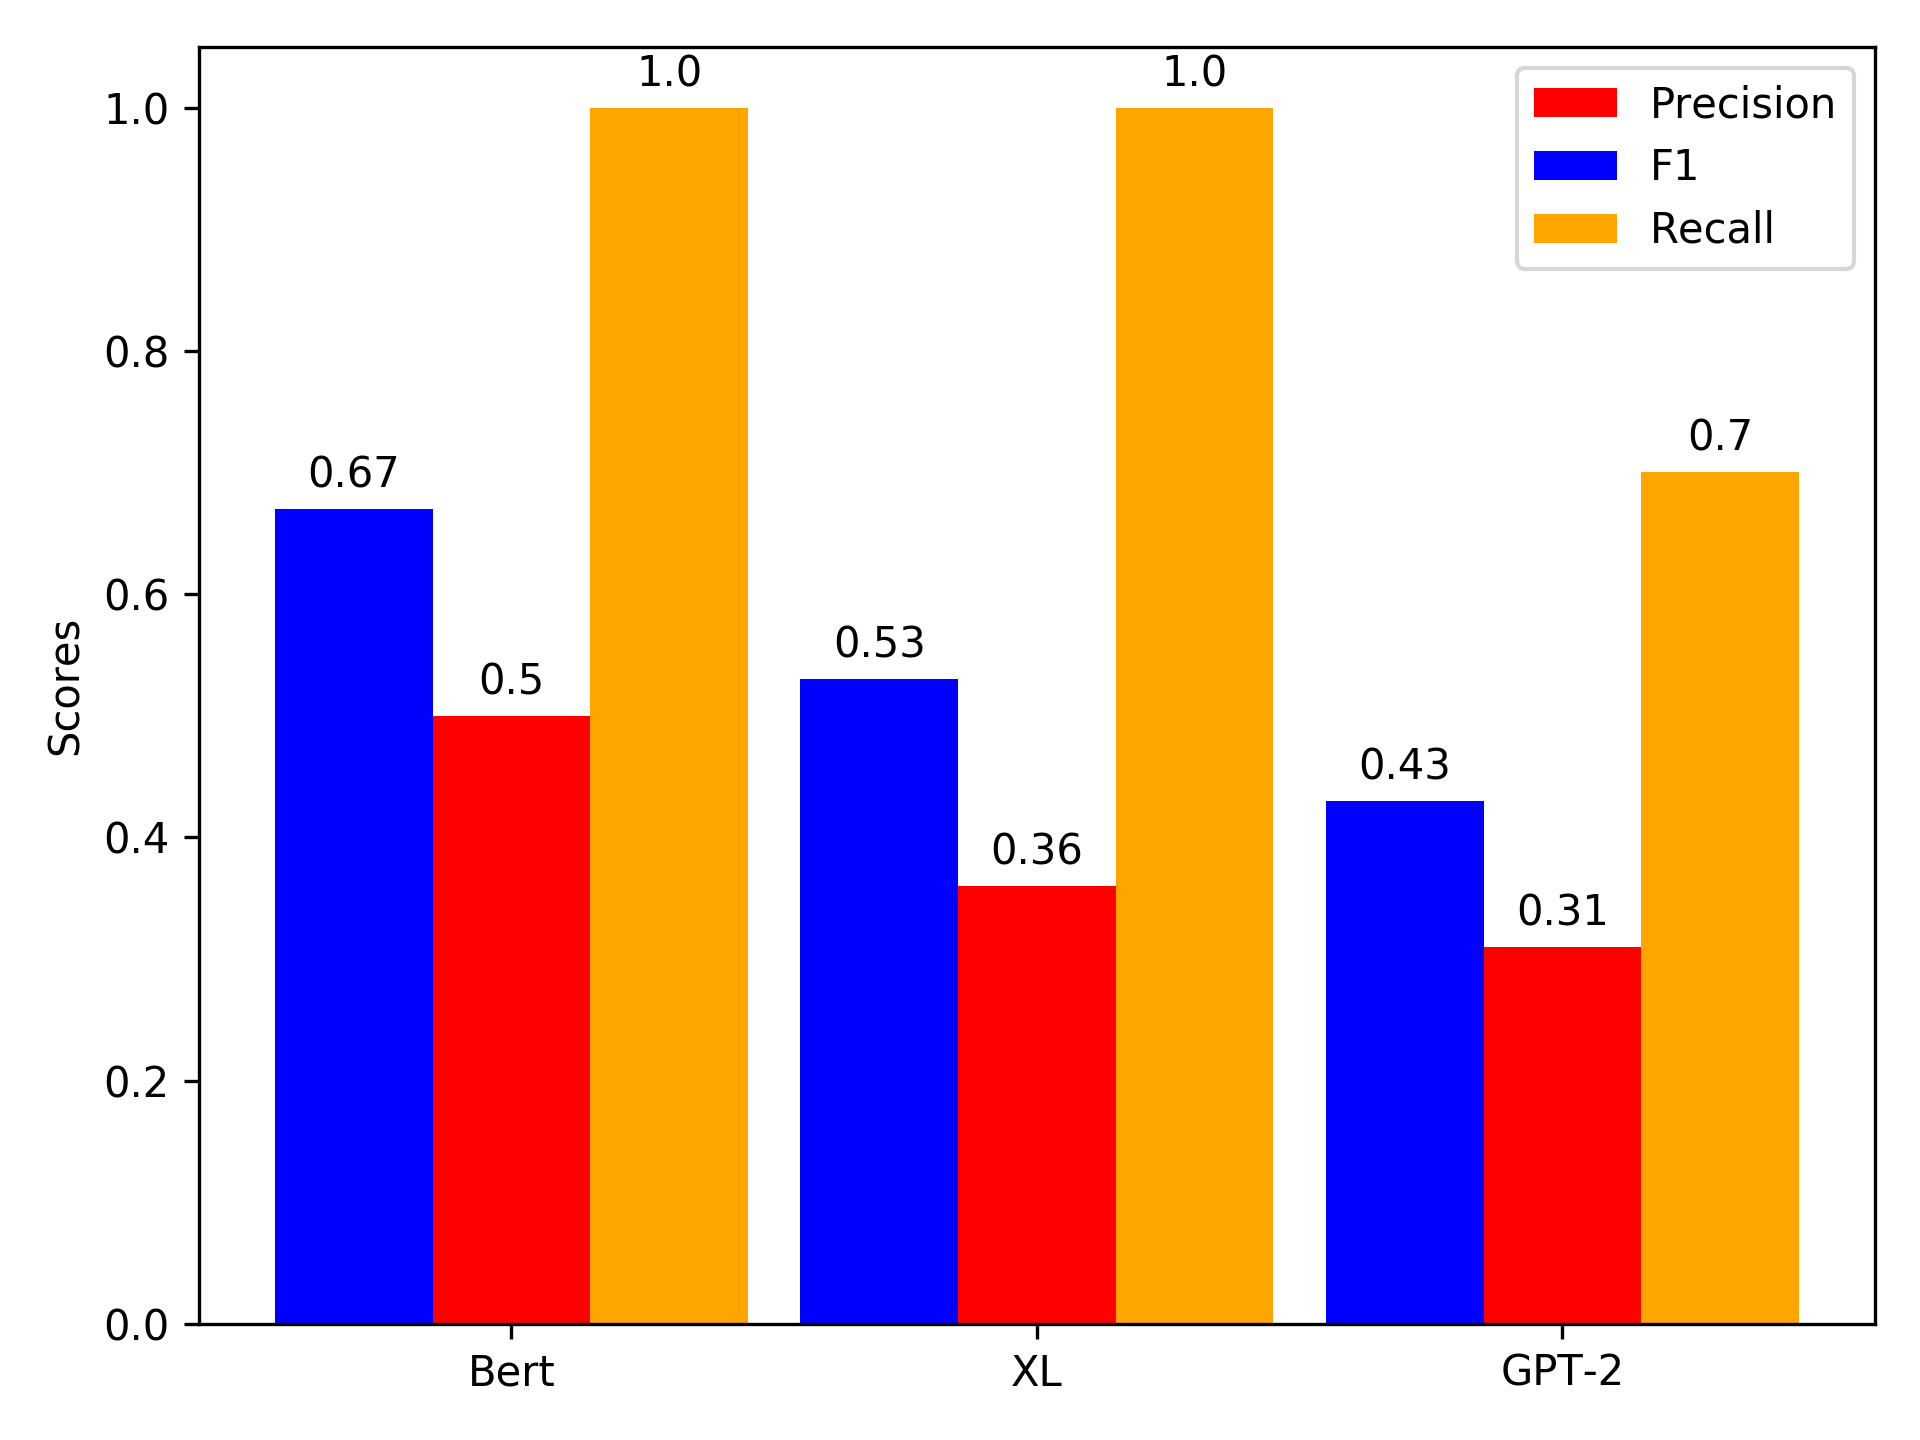
\includegraphics[trim={1cm 0.5cm 0cm 1cm}, width=0.322\textwidth]{results/average/multiclass_qualitative_average_ratio_0.15.png}}\\
\caption{\label{fig:results_multiclass_qualitative}Altering log events at different ratios, 5\% anomalies, using classification.}
\end{figure*}


\begin{figure}[H]
  \centering
  \captionsetup{justification=centering}
  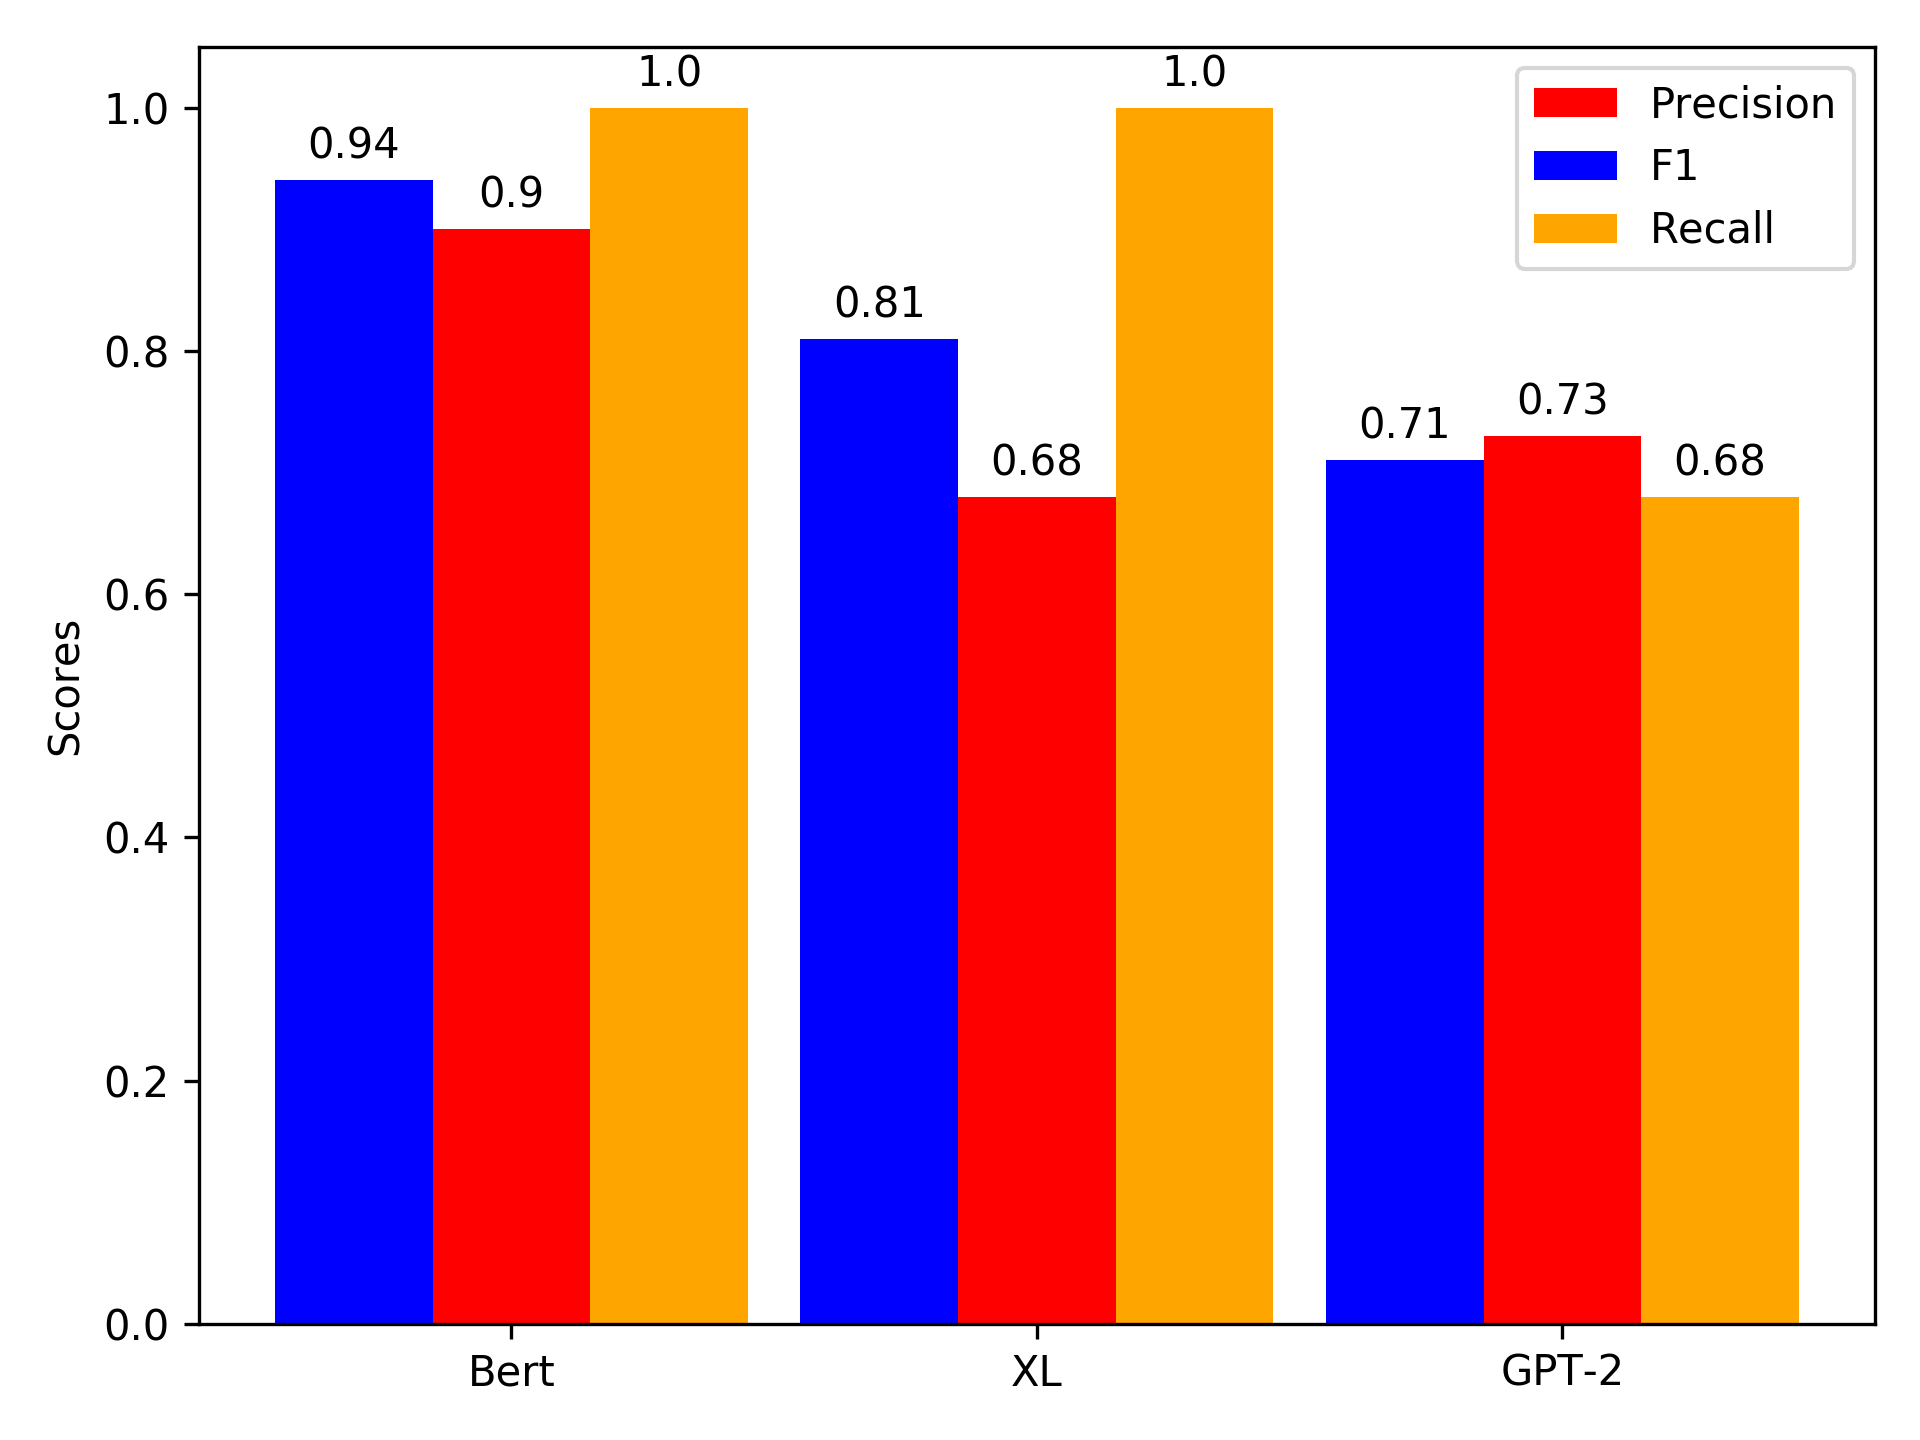
\includegraphics[width=8cm]{results/multiclass_replace_half.png}\\
  \caption{For 15\% of lines, replace 50\% of words, mark as anomaly, using classification.}
  \label{fig:replace_words_classification}
\end{figure}


% multiclass sequence length
\begin{figure}[H]
\centering
  \captionsetup{justification=centering}
  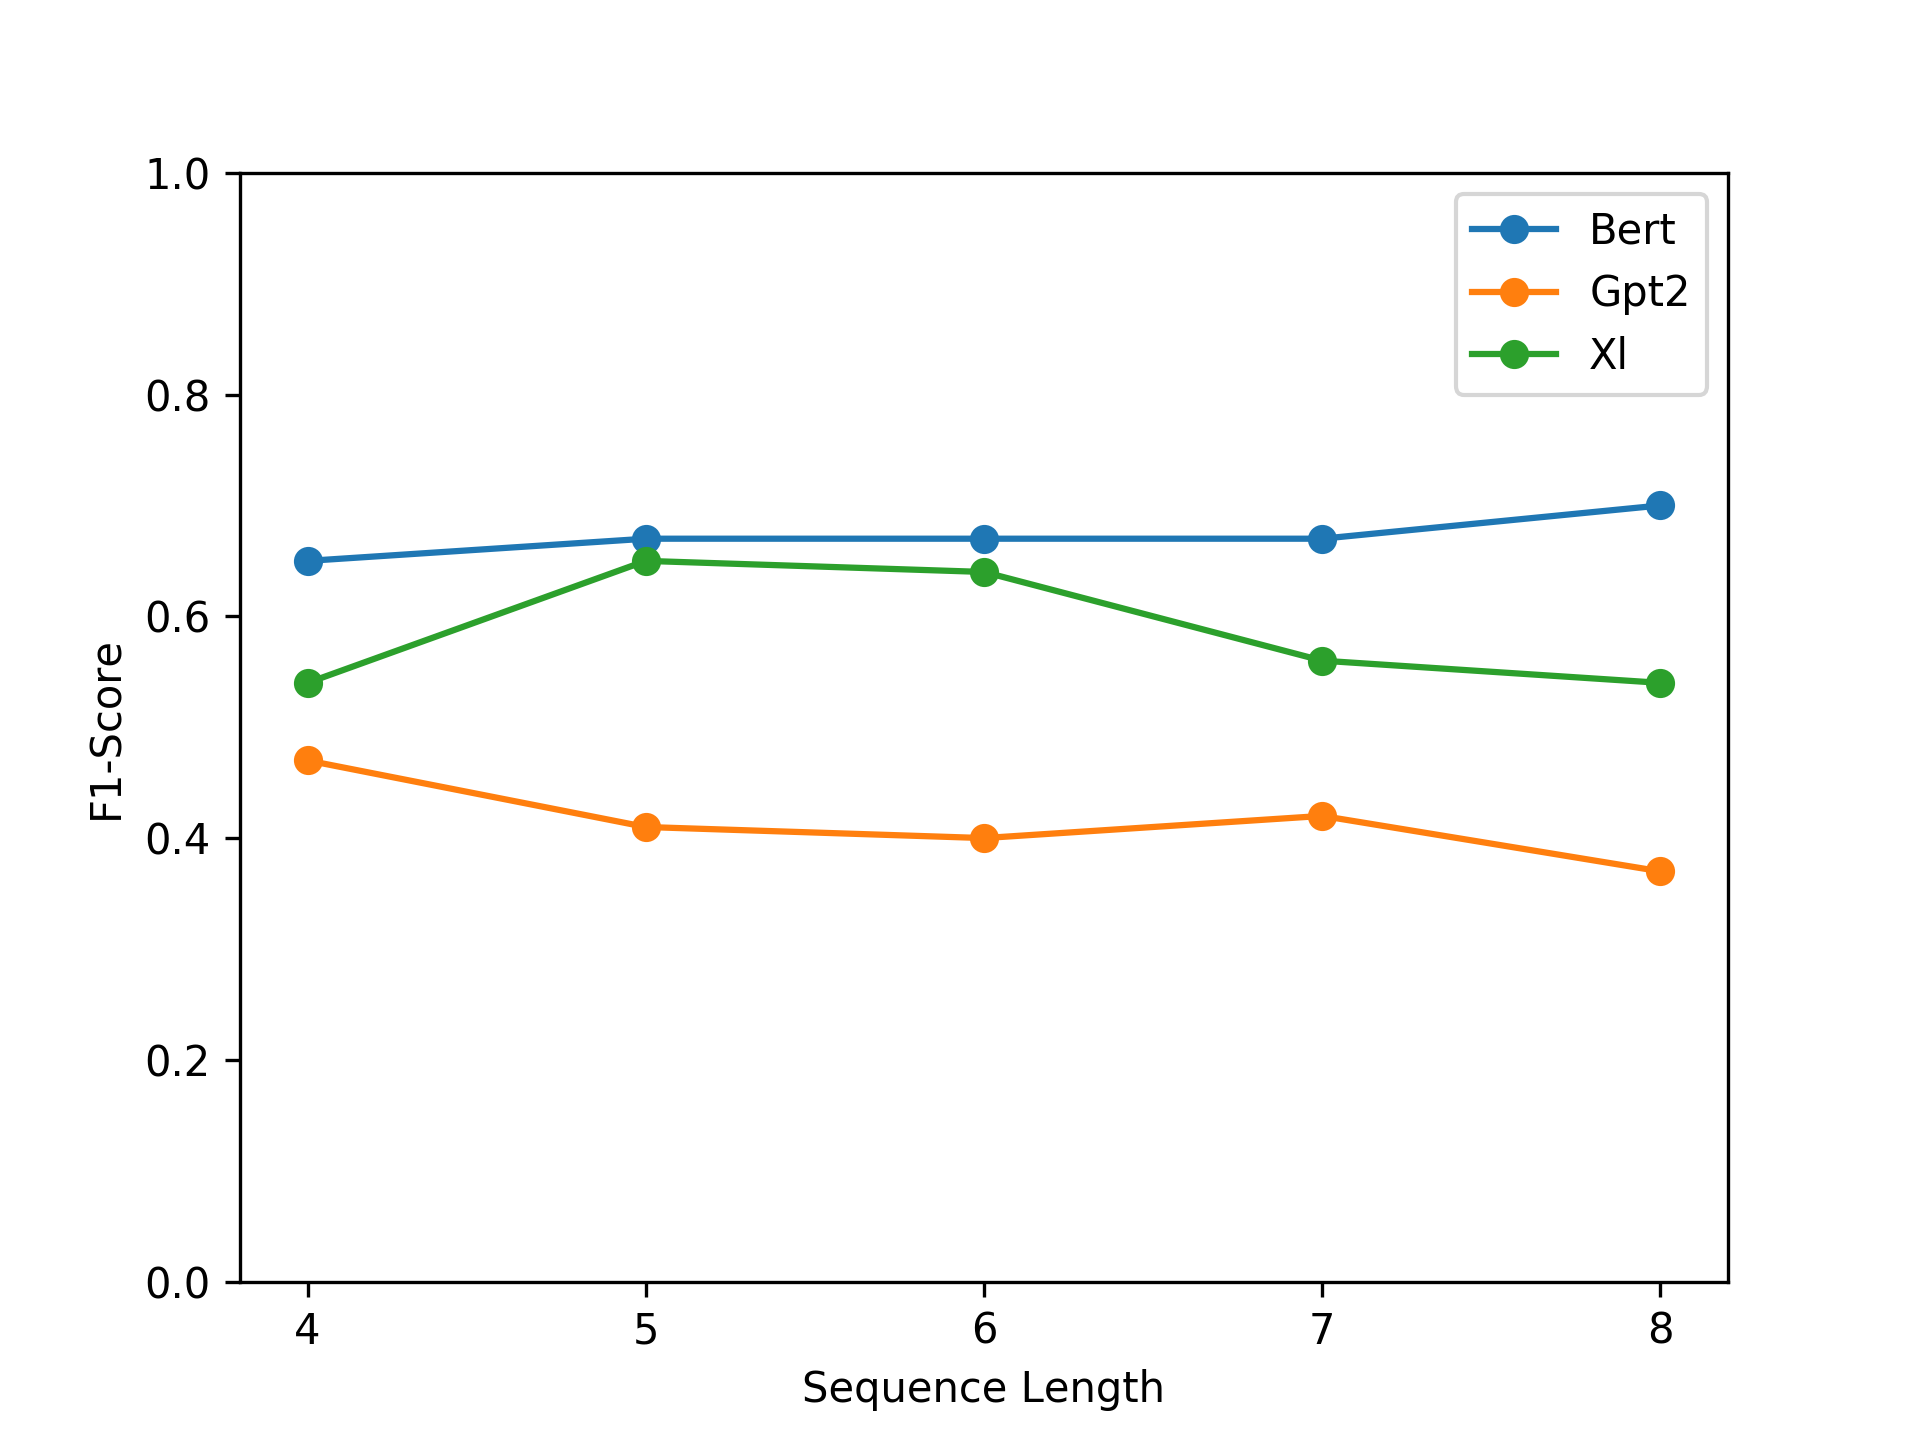
\includegraphics[width=8cm]{results/seq_len/sequence_len_classification.png}\\
  \caption{F1-Score for different input sequence lengths, with 15\% word insertion, using classification.}
  \label{fig:seq_len_classification}
\end{figure}


%%%%%
%%%%%
%%%%%

%%%%%%% TRANSFER LEARNING
%\subsection{Transfer Learning\label{sec:results_transfer}}
%In this subsection, the results of the transfer learning experiment are presented, using the classification-based approach in \ref{sec:results-classification-transfer} and the regression-based approach in \ref{sec:results-regression-transfer}.


\subsection{Transfer of knowledge using the regression-based approach \label{sec:results-regression-transfer}}

As described in \ref{sec:transfer_learning_setup}, the alterations that were injected separately in the experiments on one dataset in the last section, are now injected all at once, in order to simulate a different dataset B. Figure \ref{fig:results_transfer_regression} shows the results for alterations on 5\%, 10\% and 15\% of the log lines of all possible alterations at the same time, after 60 epochs of training on the train dataset A and 5 epochs of training on the train dataset B. 
Again, as in the previous experiments using regression, both Bert and GPT-2 achieve perfect recall values of 1.0, while XL-Transformers only achieves around 0.49. With regards to F1-score and precision, GPT-2 performs far better than Bert and XL-Transformers, yet Bert achieves a good F1-score of 0.95 and precision of 0.9 for 5\% alteration ratios, but degrades substantially for 10\% and 15\% to around 0.67 in F1-score and around 0.5 in precision. XL-Transformers shows an F1-score of 0.41 for 5\% alterations, 0.34 for 10\% alterations and 0.26 for 15\% alterations, and precision of 0.33 for 5\% alterations, 0.28 for 10\% alterations and 0.18 for 15\% alterations.

It is clearly visible, that Bert and XL-Transformers are both degrading in all metrics with increasing alteration ratio, yet GPT-2 achieves good results even with an increasing alteration ratio.

\begin{comment}
\begin{figure}[h]
  \centering
  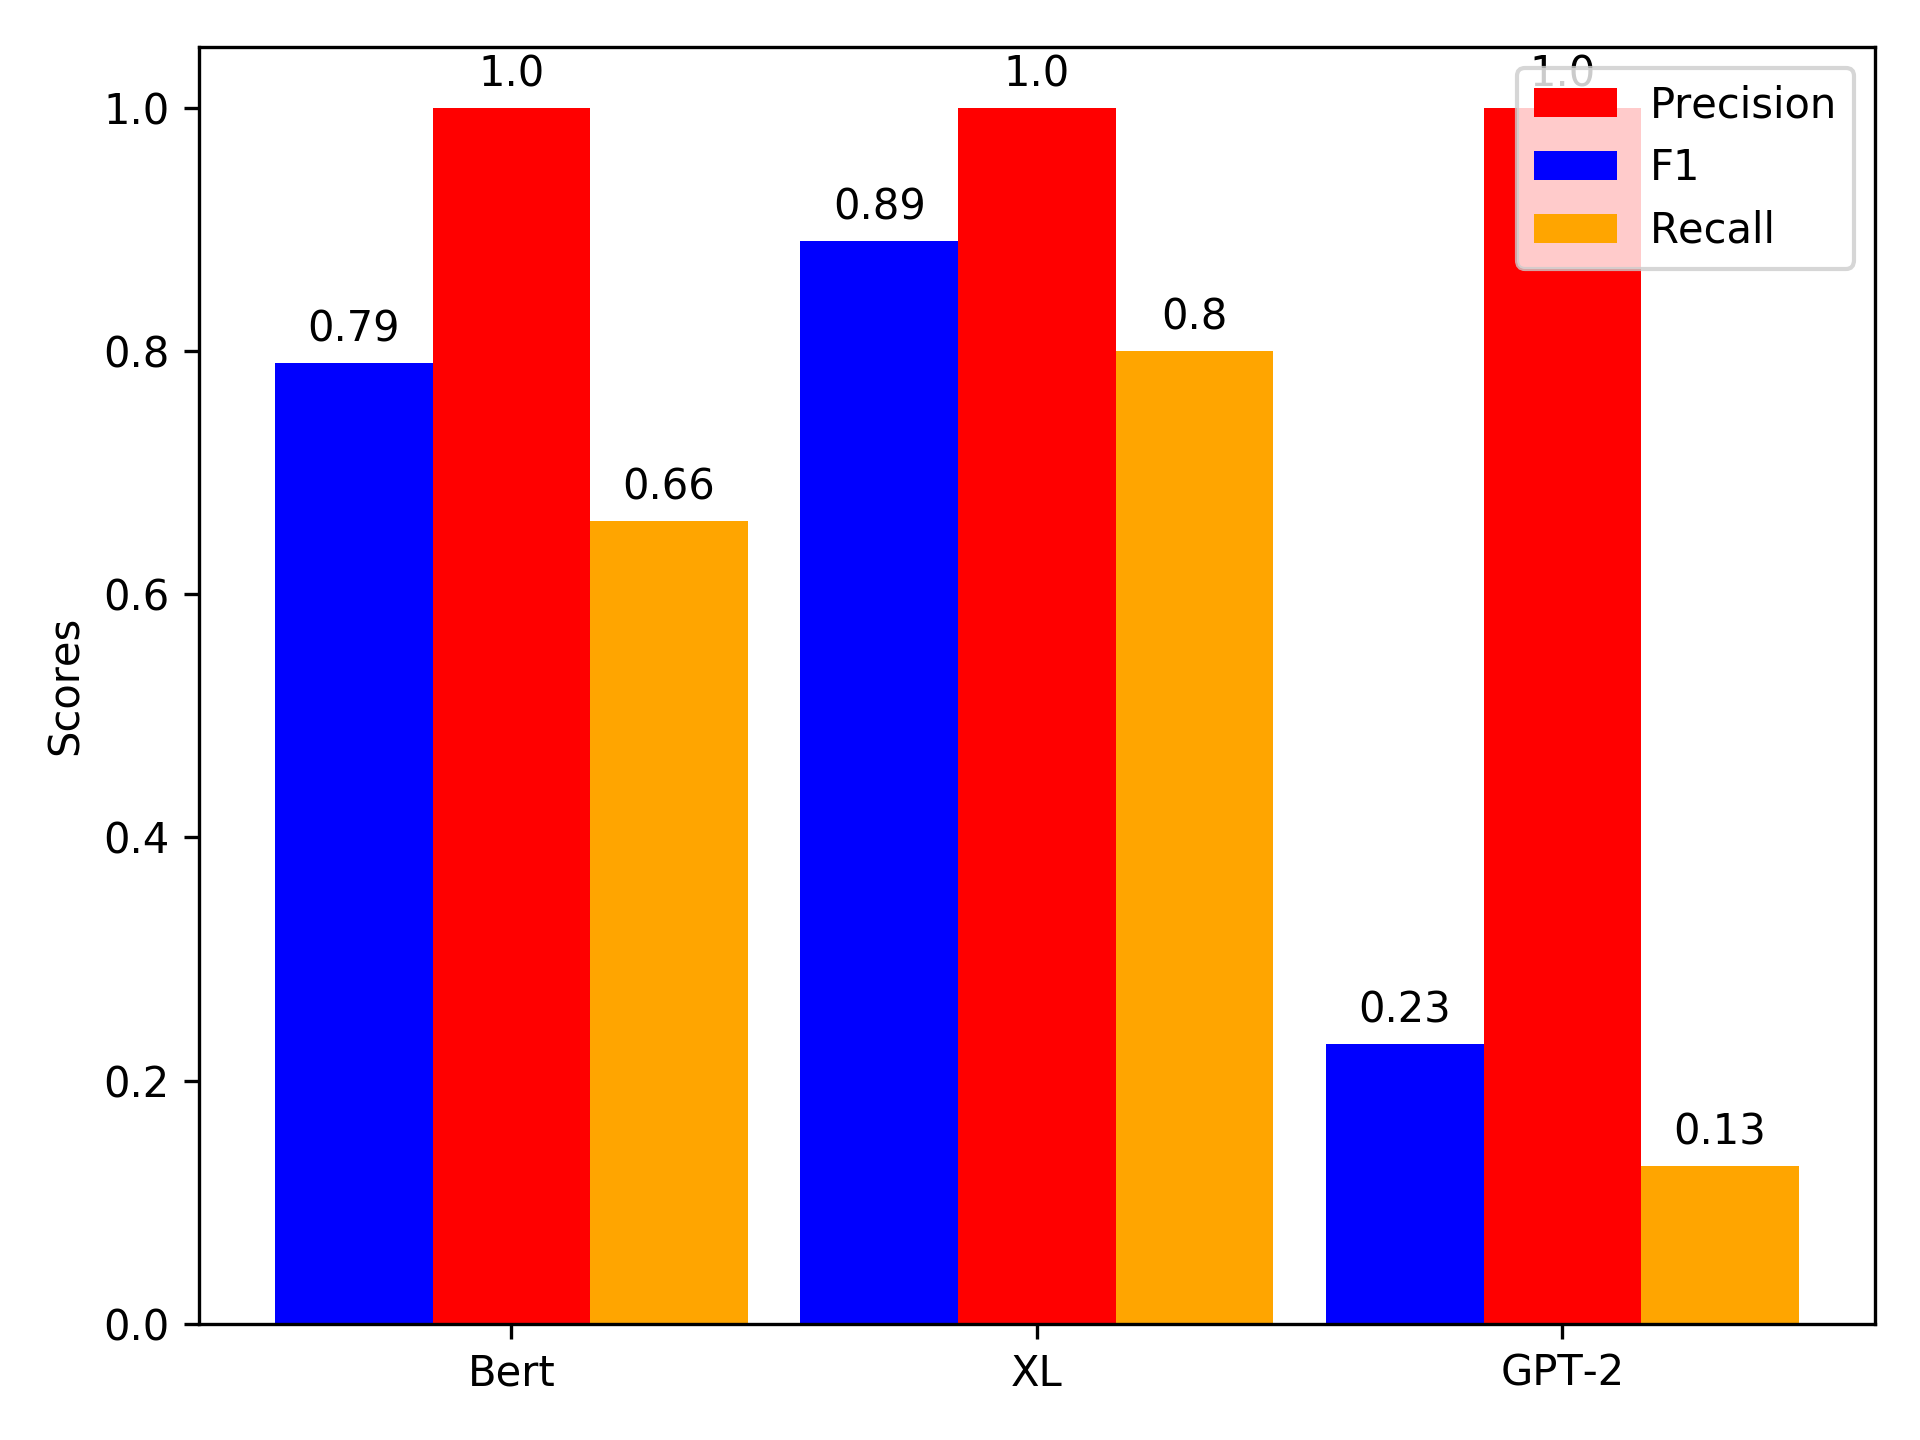
\includegraphics[width=6cm,height=4.5cm]{results/transfer/transfer_regression_reverse.png}\\
  \caption{Scores for detecting reversed order of log events for transfer learning, using regression.}
  \label{fig:regression_transfer_reverse}
\end{figure}
\end{comment}

\begin{figure*}[ht!]
  \centering
  \captionsetup{justification=centering}
   \subfloat[5\% alteration\label{fig:results_transfer_regression_0.05}]{%
      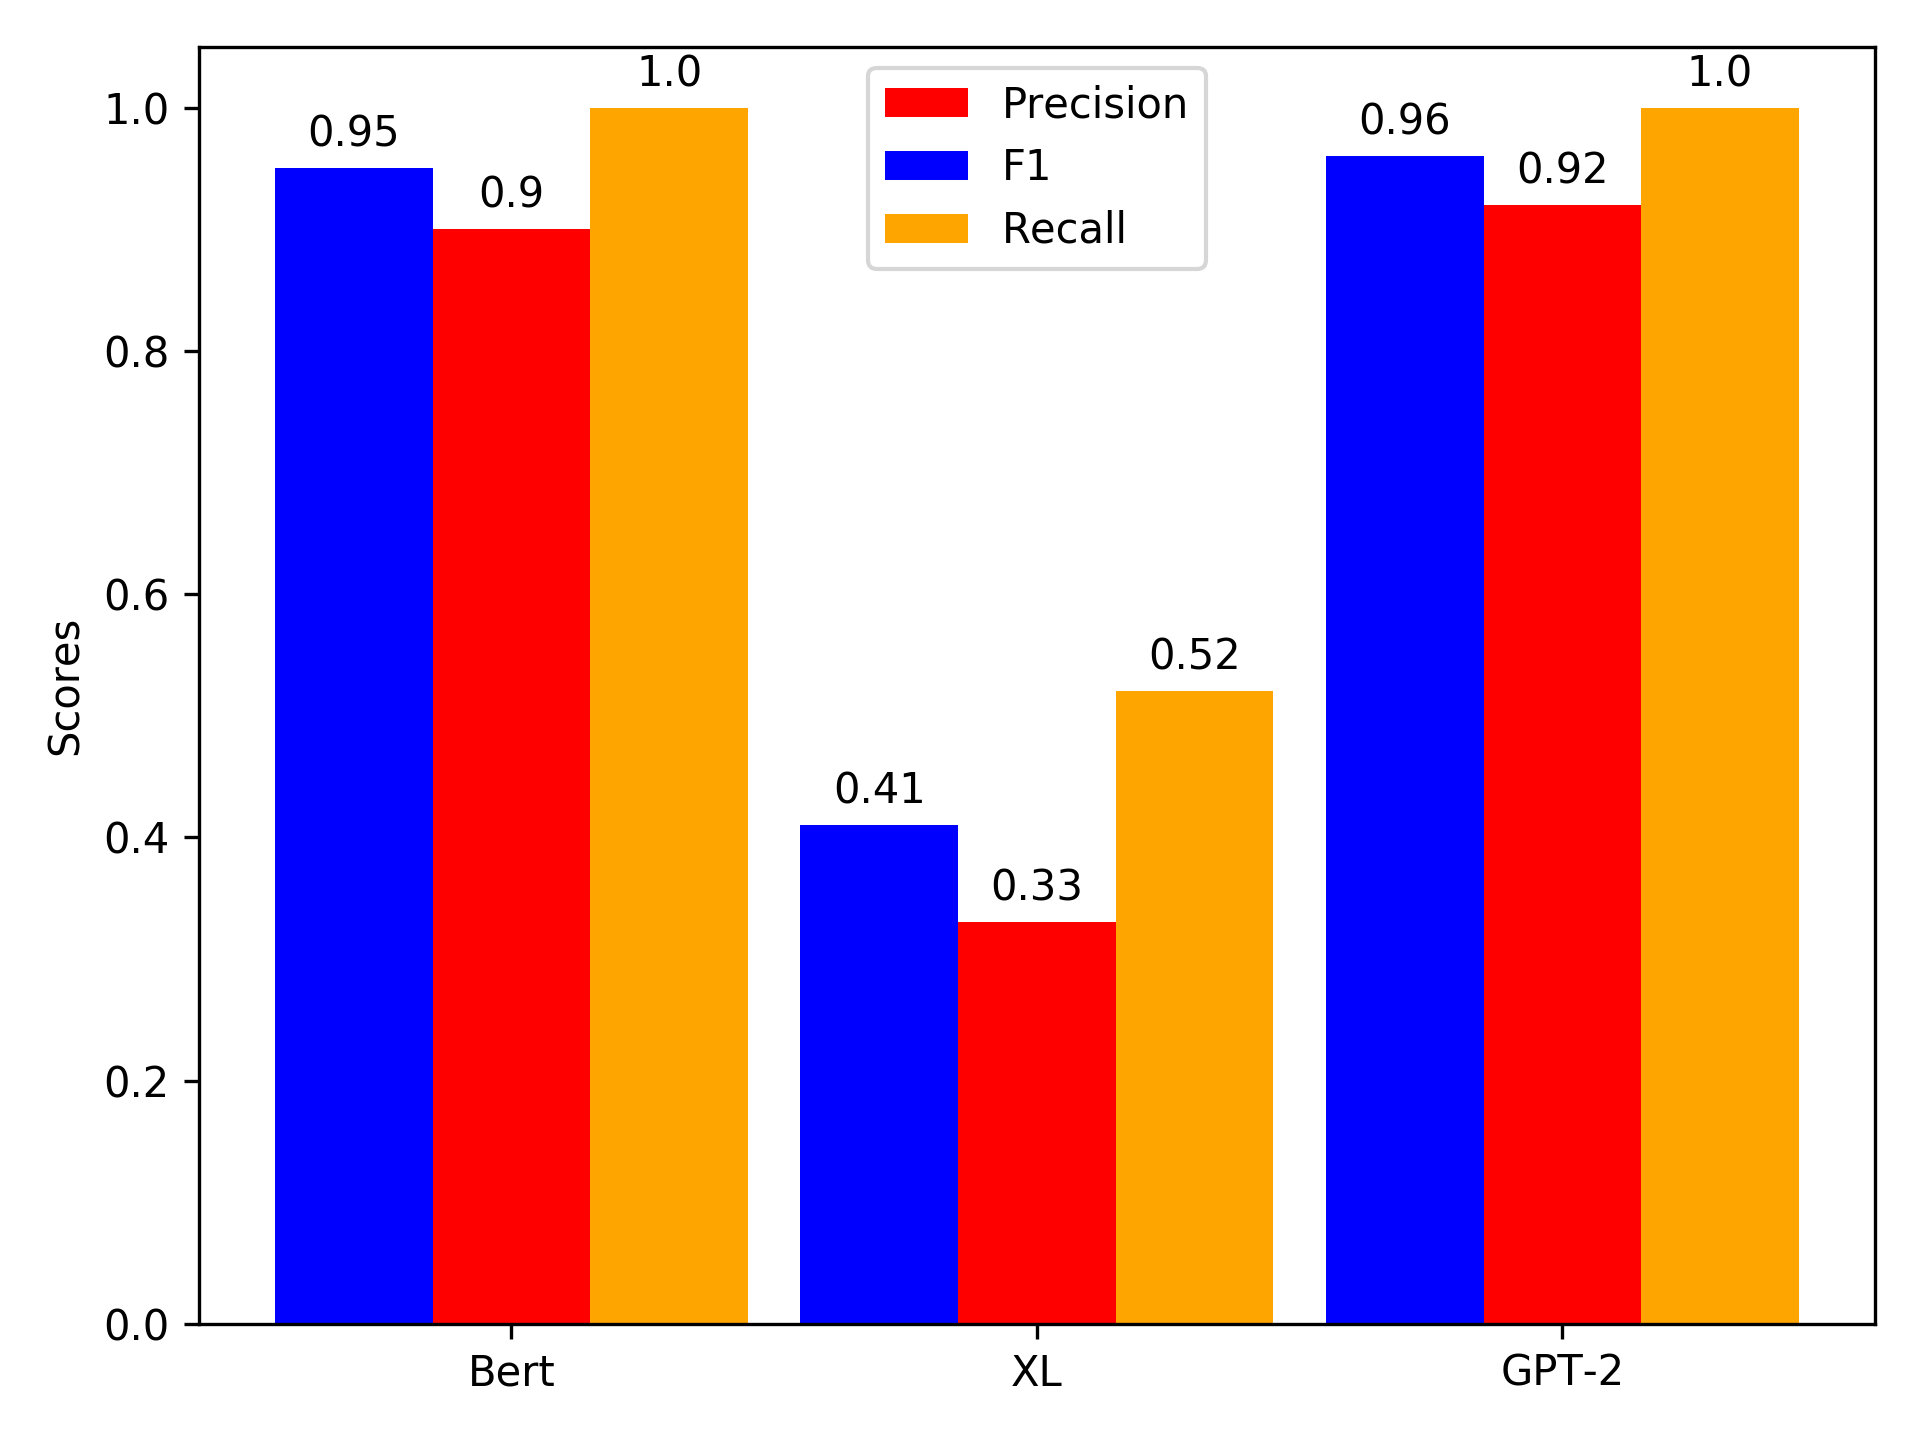
\includegraphics[trim={1cm 0.5cm 0cm 1cm}, width=0.322\textwidth]{results/transfer/transfer_regression_0.05_ratio.png}}
\hspace{\fill}
   \subfloat[10\% alteration\label{fig:results_transfer_regression_0.10} ]{%
      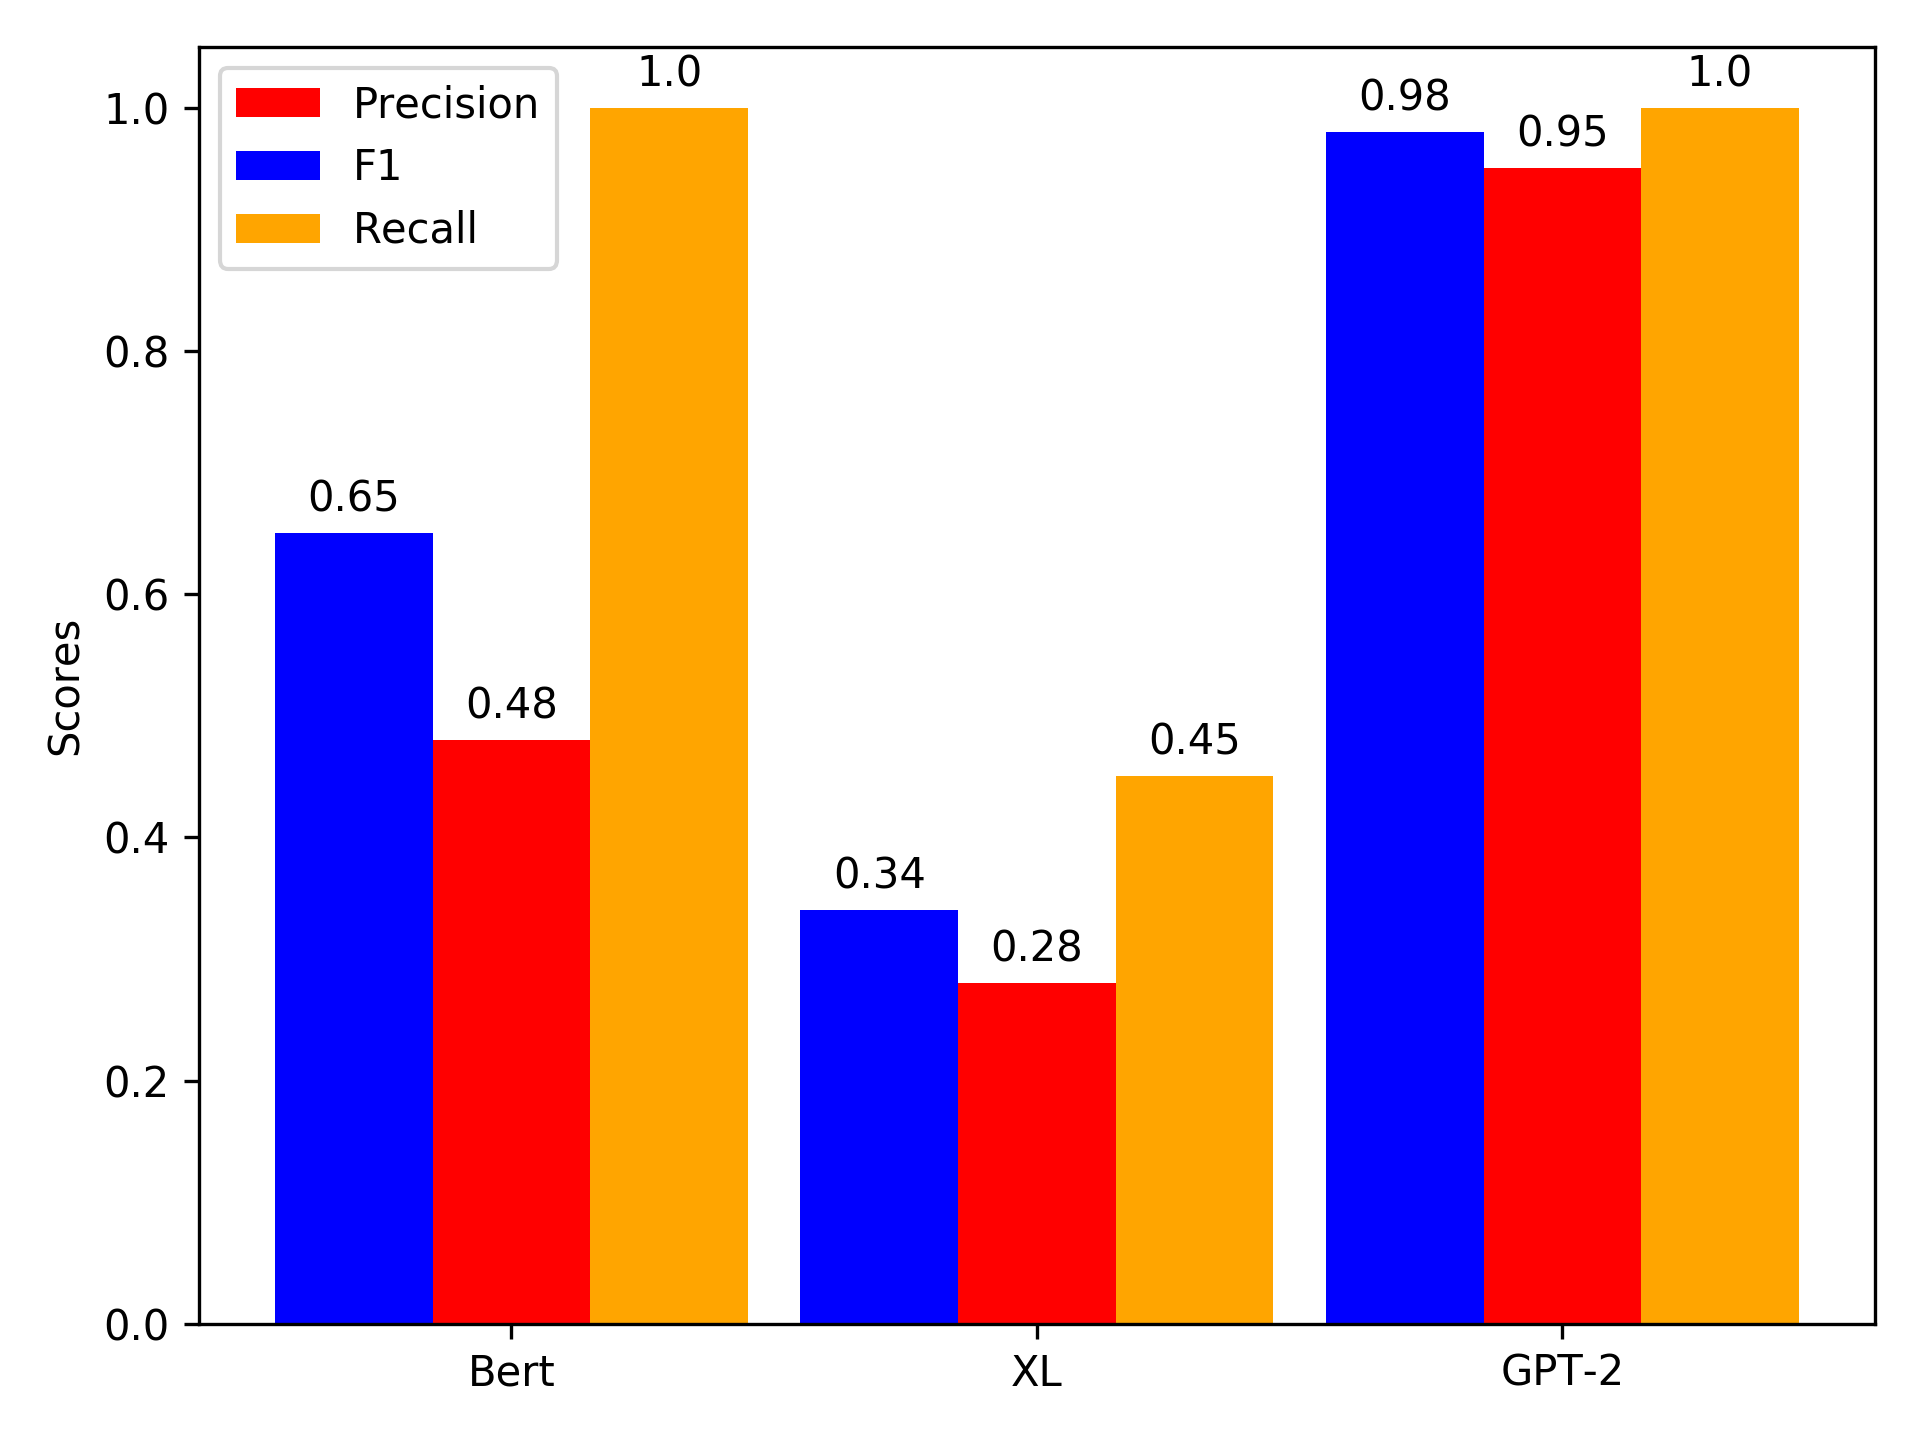
\includegraphics[trim={1cm 0.5cm 0cm 1cm}, width=0.322\textwidth]{results/transfer/transfer_regression_0.1_ratio.png}}
\hspace{\fill}
   \subfloat[15\% alteration\label{fig:results_transfer_regression_0.15}]{%
      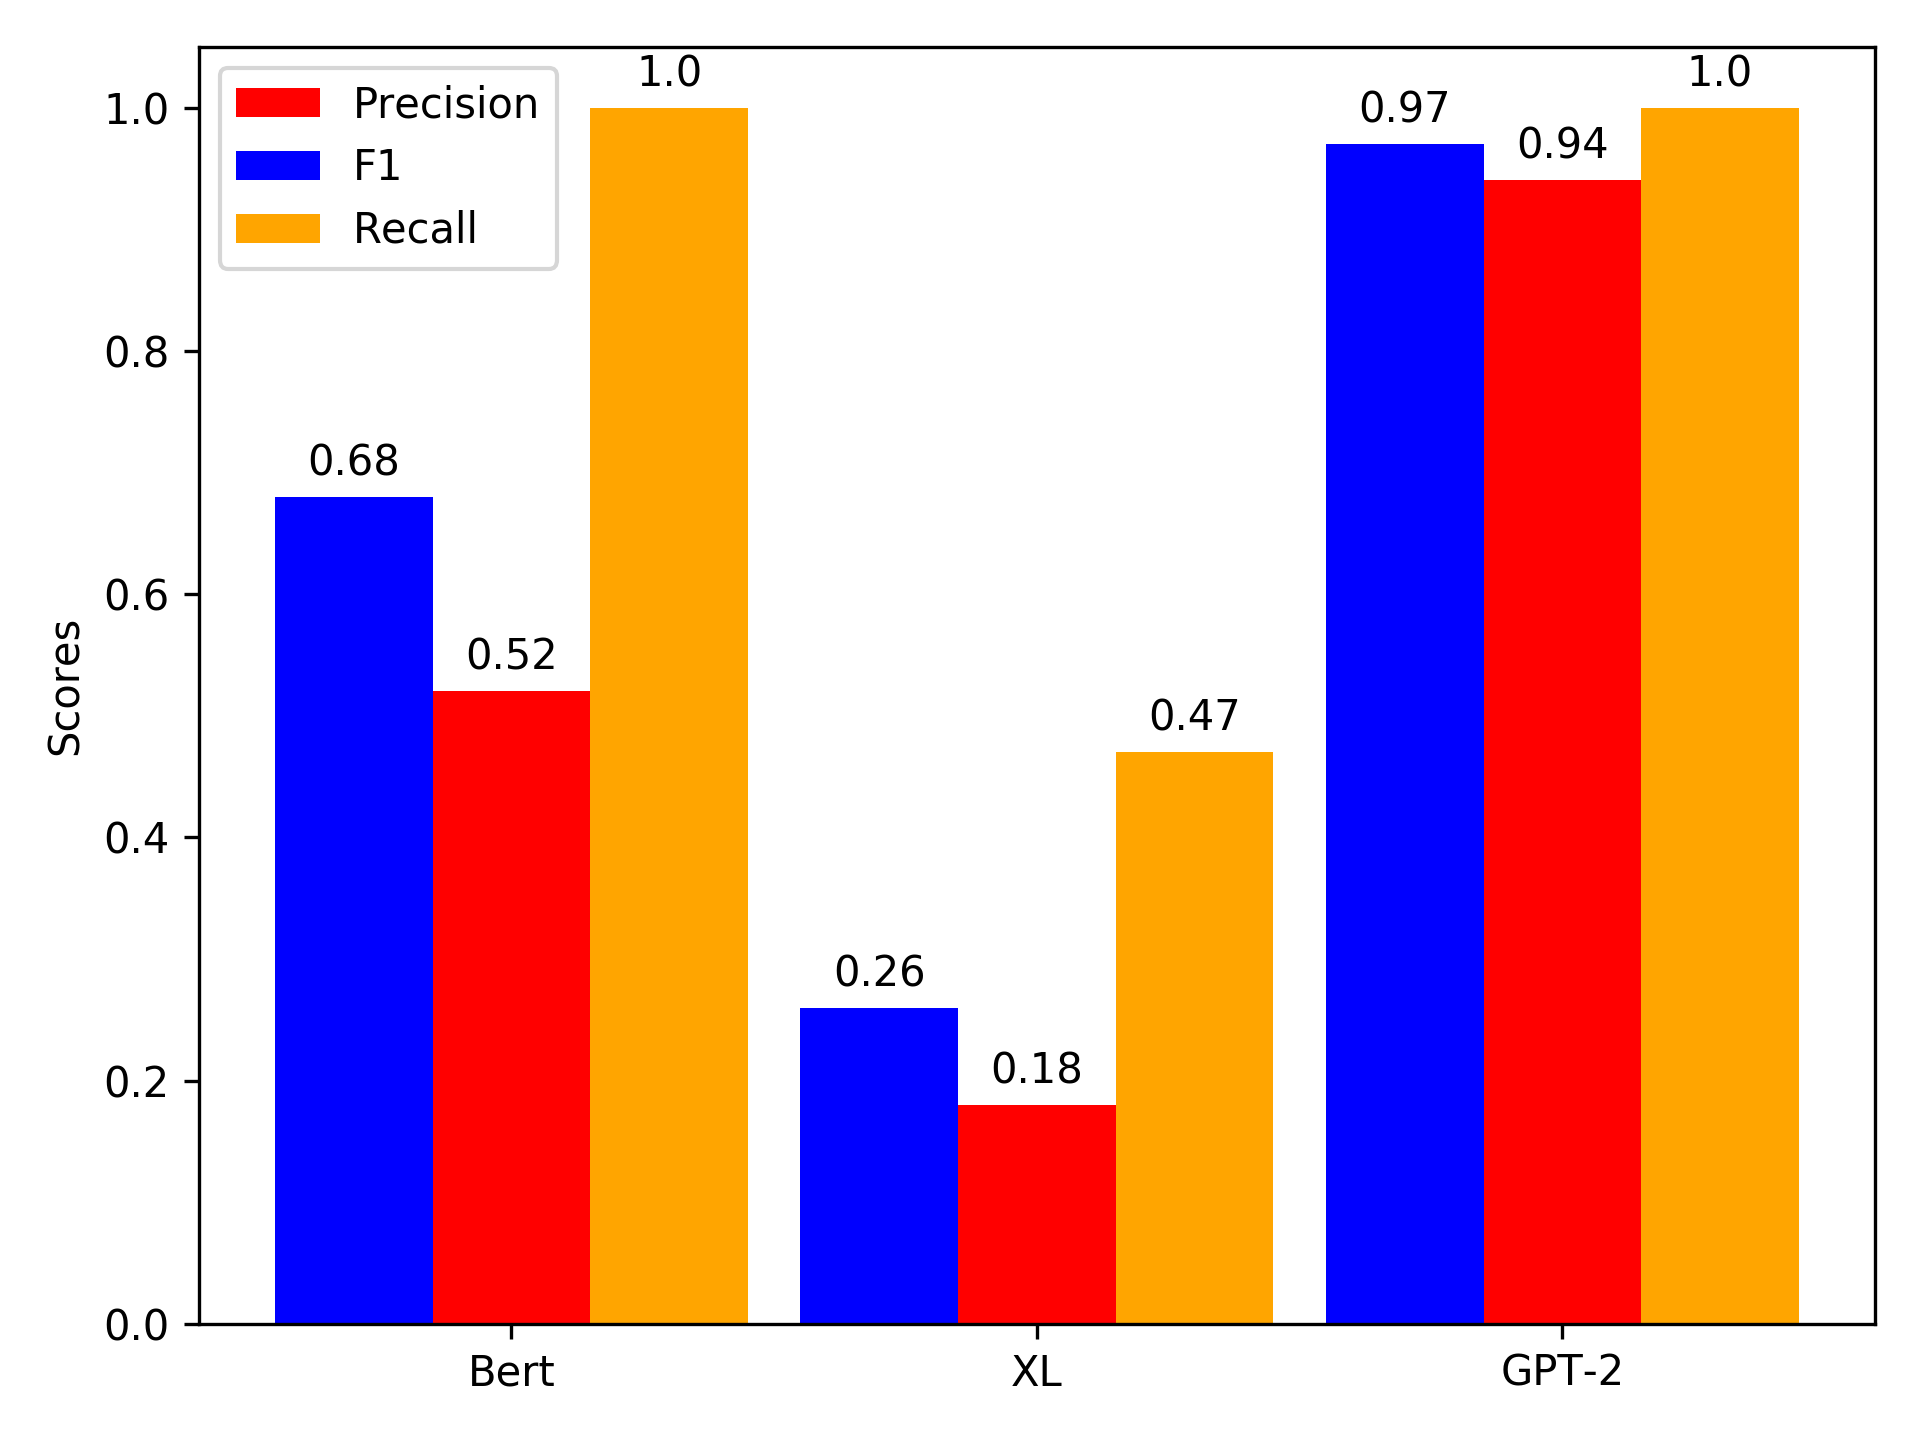
\includegraphics[trim={1cm 0.5cm 0cm 1cm}, width=0.322\textwidth]{results/transfer/transfer_regression_0.15_ratio.png}}\\
\caption{\label{fig:results_transfer_regression}Transfer of knowledge with different ratios of alteration, 5\% anomalies, using regression.}
\end{figure*}


Figure \ref{fig:results_transfer_regression_per_epoch} depicts the development of the metrics of detecting anomalies for every additional epoch of training on dataset B. It is clearly visible, that XL-Transformers improves the most per epoch, although starting from a relatively low starting point, whereas Bert has a smaller increase per training epoch. The results of GPT-2 do not change much per epoch, but start at a very high level already, corresponding to the findings already made on GPT-2 using regression in \ref{sec:results-regression}. 
These findings are confirmed by the ROC curve plots which can be seen in figure \ref{fig:results_transfer_regression_roc}, showing nearly perfect results for GPT-2, very good results for Bert and far less satisfying results for XL-Transformers.

\begin{figure*}[ht!]
\centering
  \captionsetup{justification=centering}
   \subfloat[Bert\label{fig:results_transfer_regression_per_epoch_0.05}]{%
      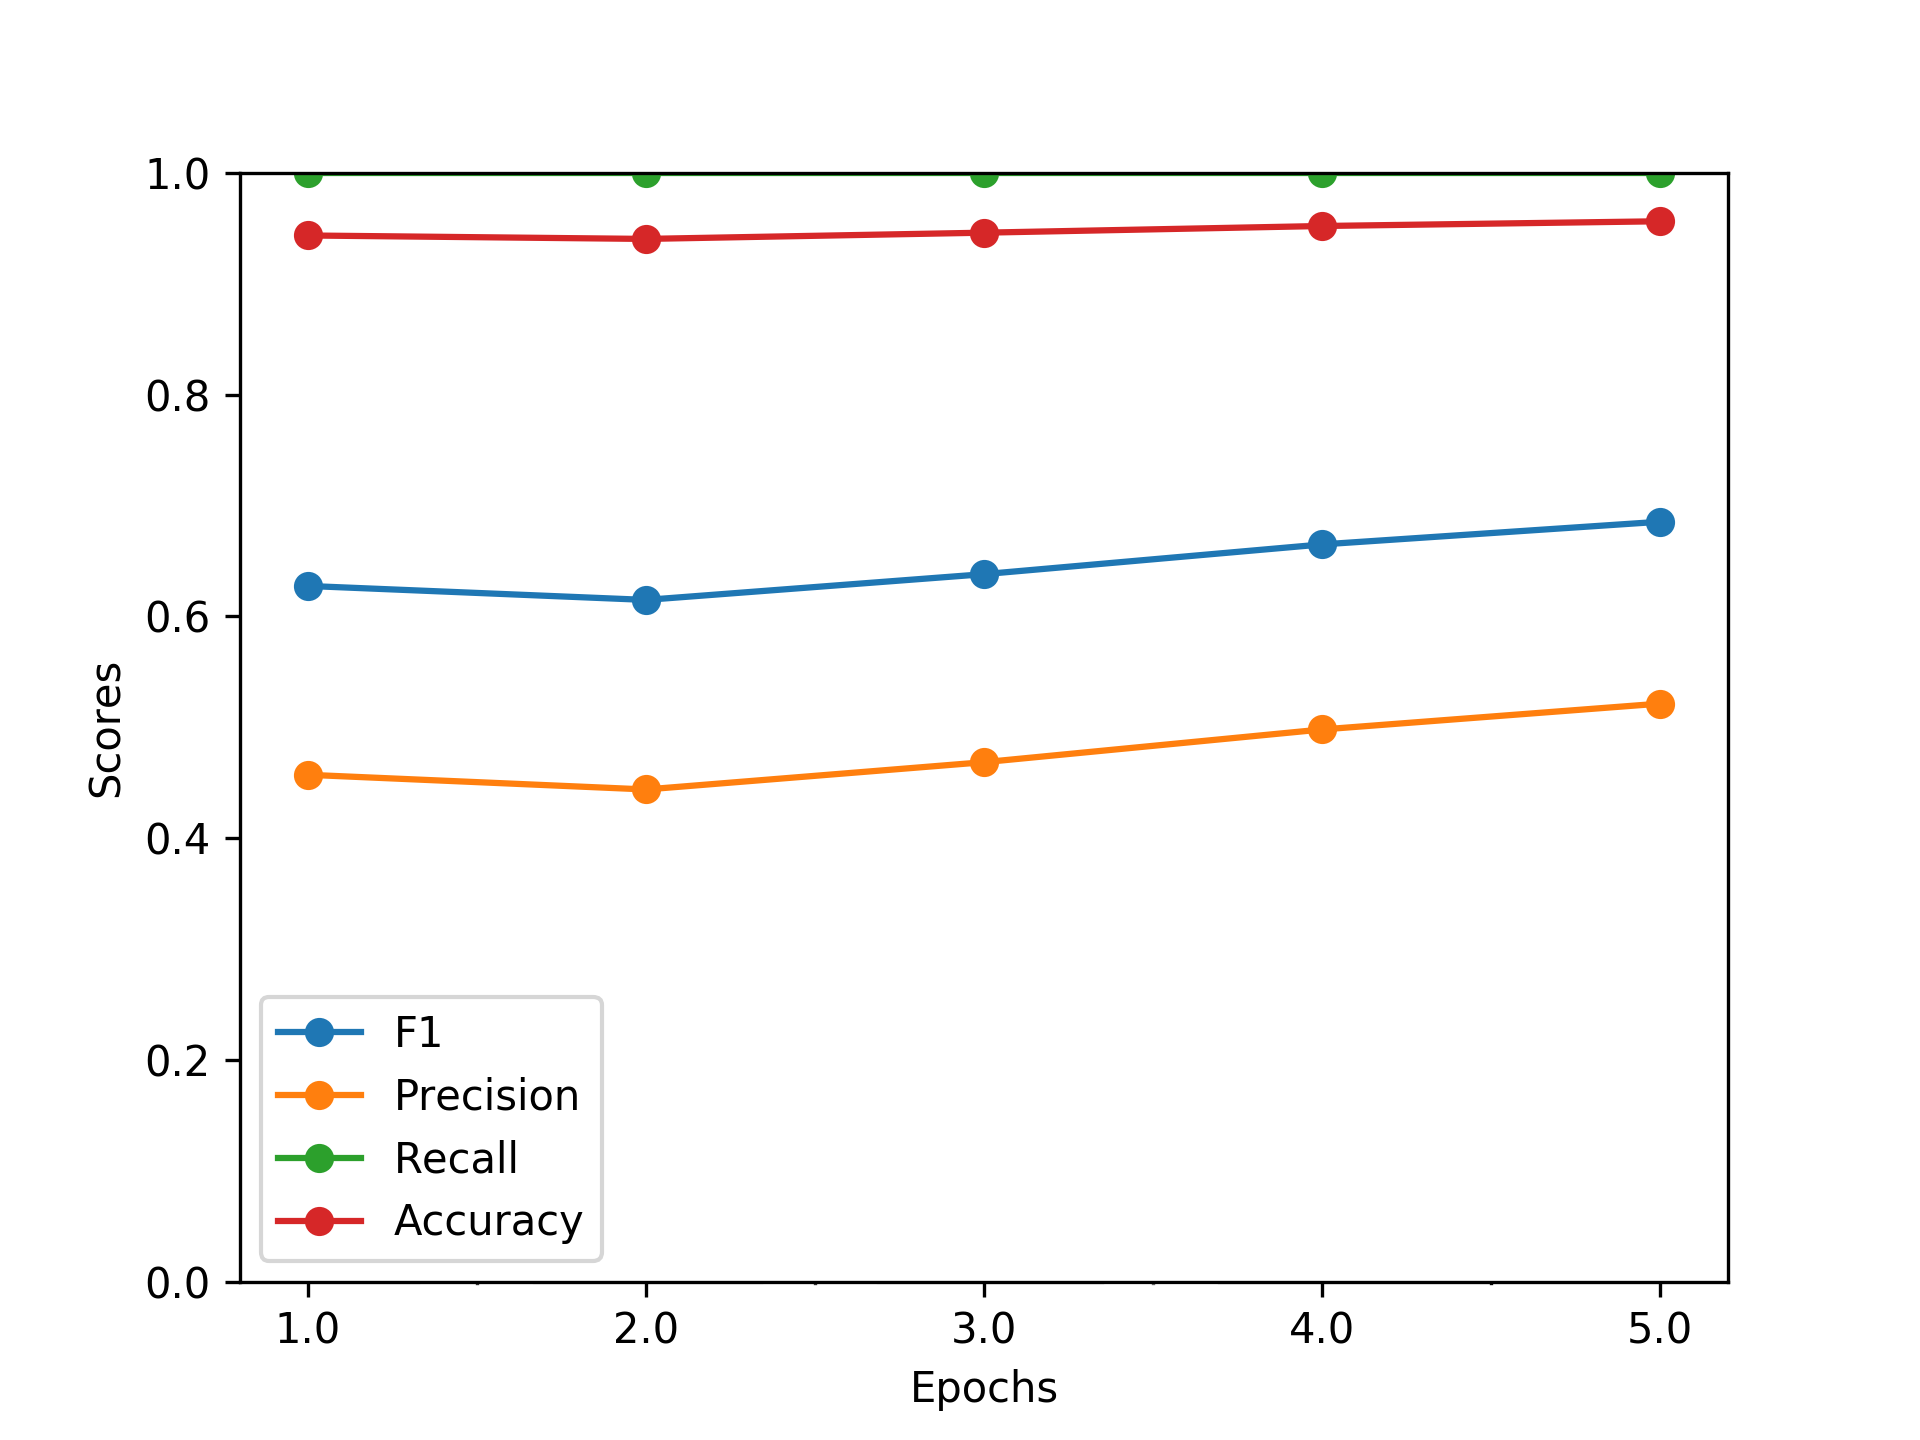
\includegraphics[trim={1cm 0.5cm 0cm 1cm}, width=0.322\textwidth]{results/transfer/bert_regression_0.15_transfer_metrics_per_epoch.png}}
\hspace{\fill}
   \subfloat[GPT-2\label{fig:results_transfer_regression_per_epoch_0.10} ]{%
      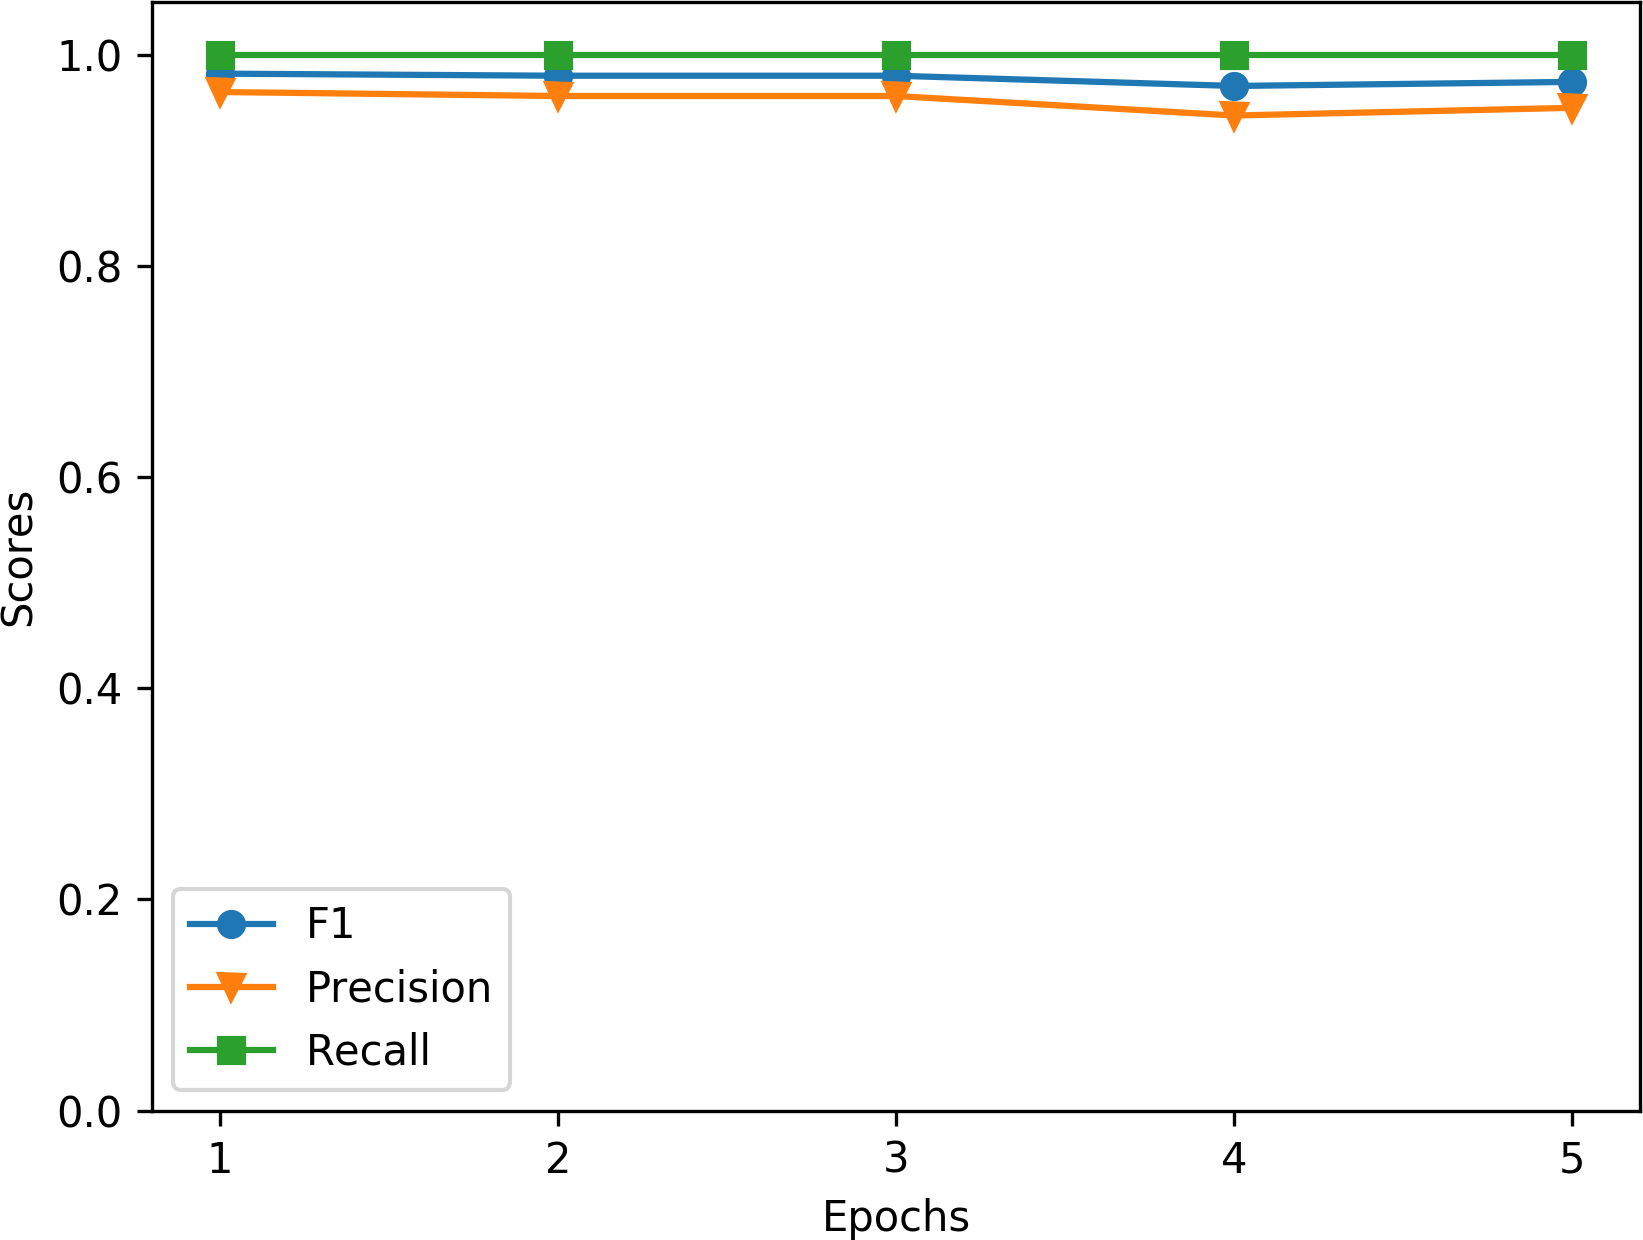
\includegraphics[trim={1cm 0.5cm 0cm 1cm}, width=0.322\textwidth]{results/transfer/gpt_regression_0.15_transfer_metrics_per_epoch.png}}
\hspace{\fill}
   \subfloat[XL\label{fig:results_transfer_regression_per_epoch_0.15}]{%
      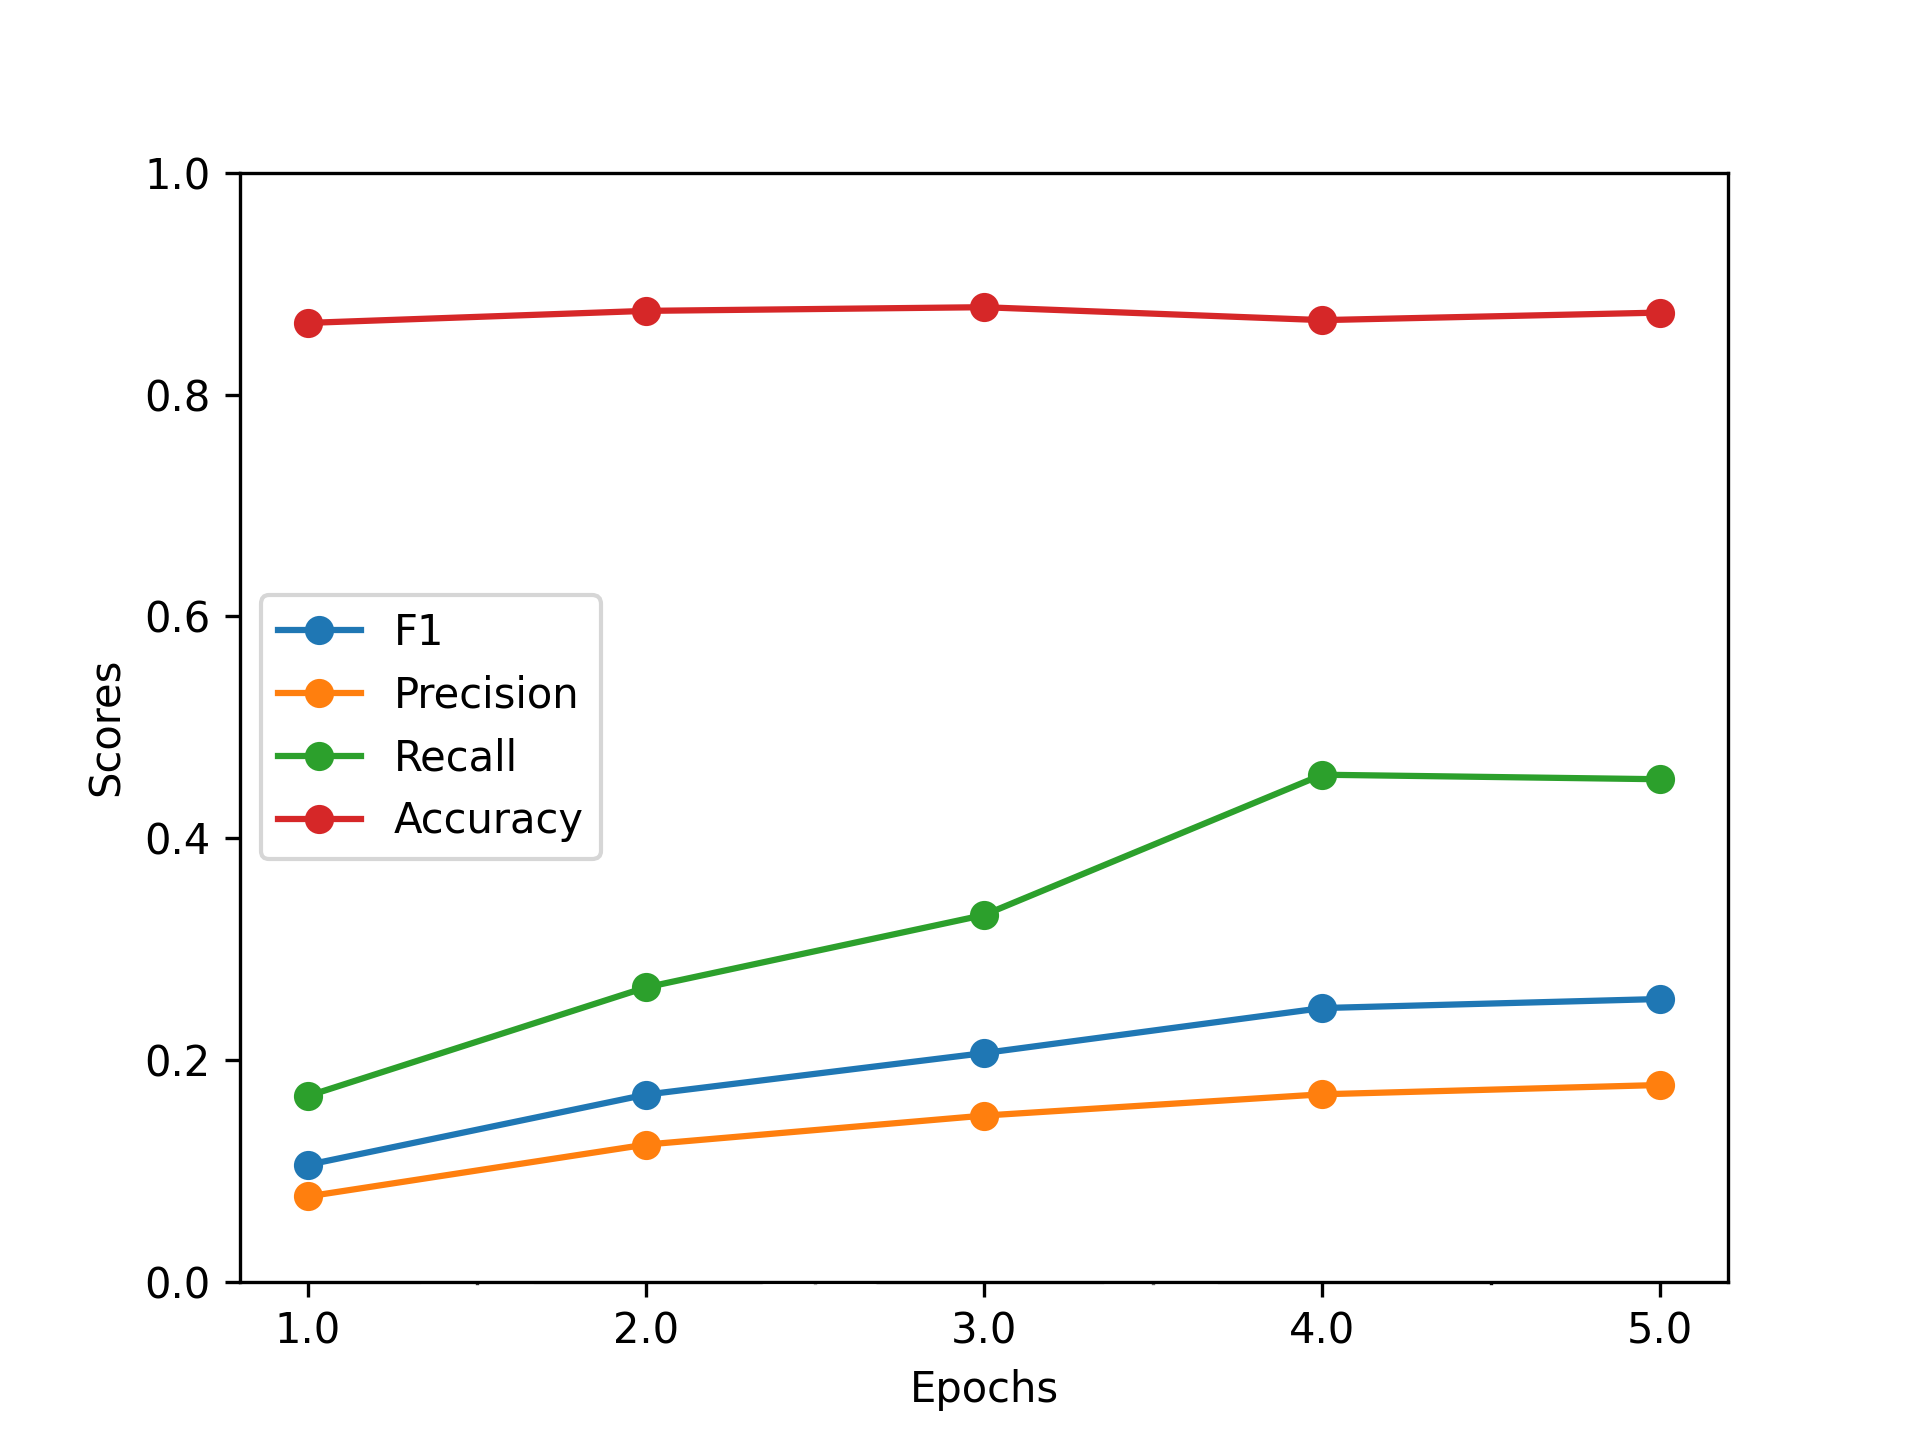
\includegraphics[trim={1cm 0.5cm 0cm 1cm}, width=0.322\textwidth]{results/transfer/xl_regression_0.15_transfer_metrics_per_epoch.png}}\\
\caption{\label{fig:results_transfer_regression_per_epoch}Improvement of metrics for transfer of knowledge per additional learning epoch, using regression.}
\end{figure*}

%\begin{comment}
\begin{figure*}[ht!]
\centering
  \captionsetup{justification=centering}
   \subfloat[Bert\label{fig:roc_curve_bert_transfer_regression}]{%
      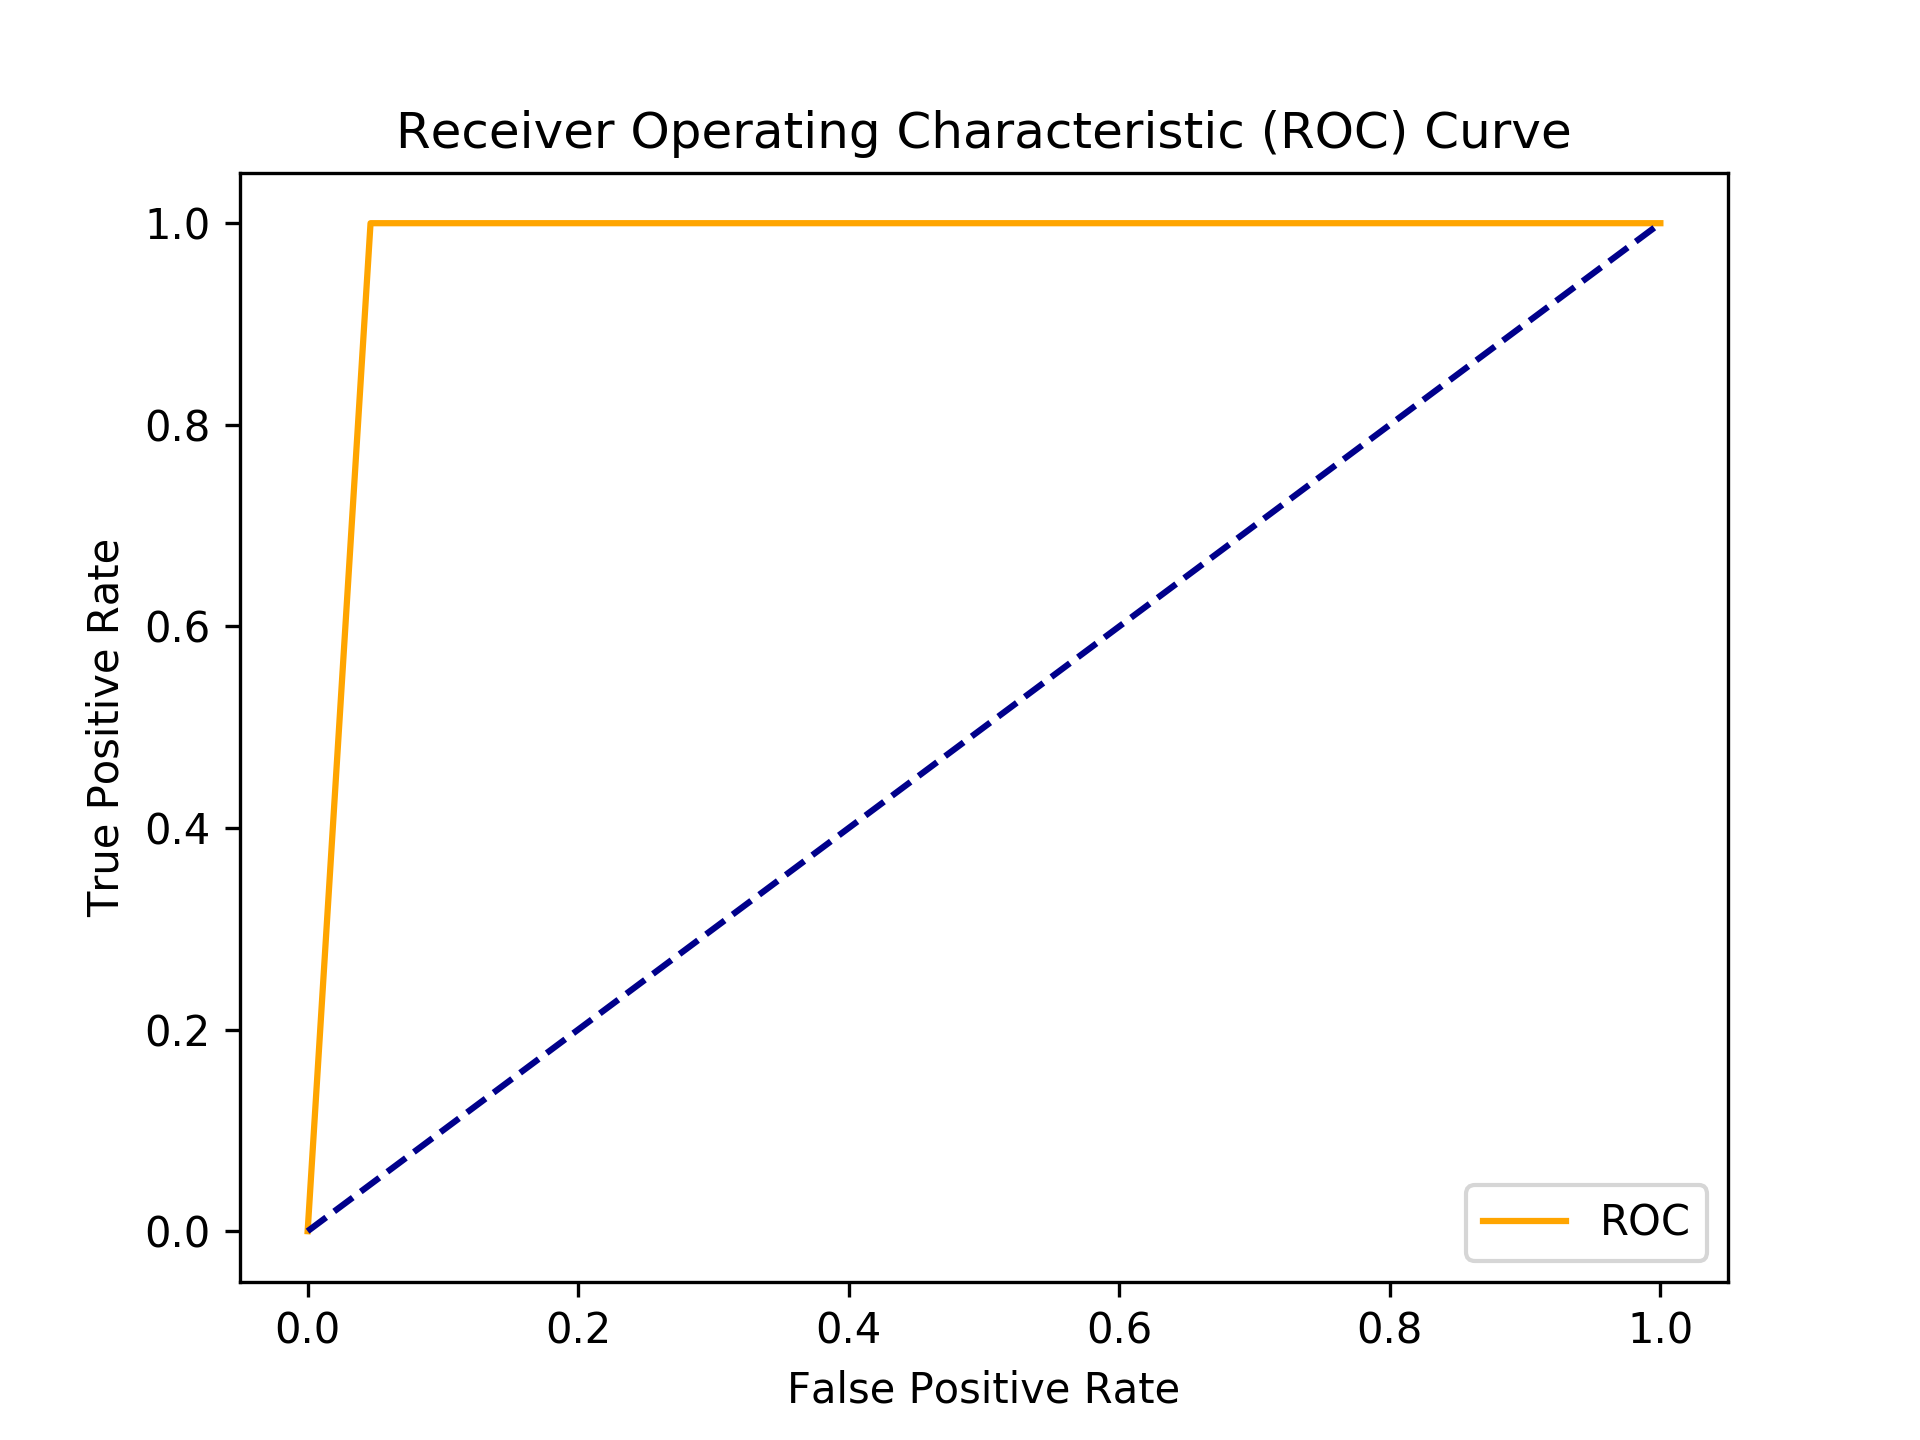
\includegraphics[trim={1cm 0.5cm 0cm 1cm}, width=0.322\textwidth]{results/transfer/roc_curve_transfer_regression_bert_0.15.png}}
\hspace{\fill}
   \subfloat[GPT-2\label{fig:roc_curve_gpt_transfer_regression} ]{%
      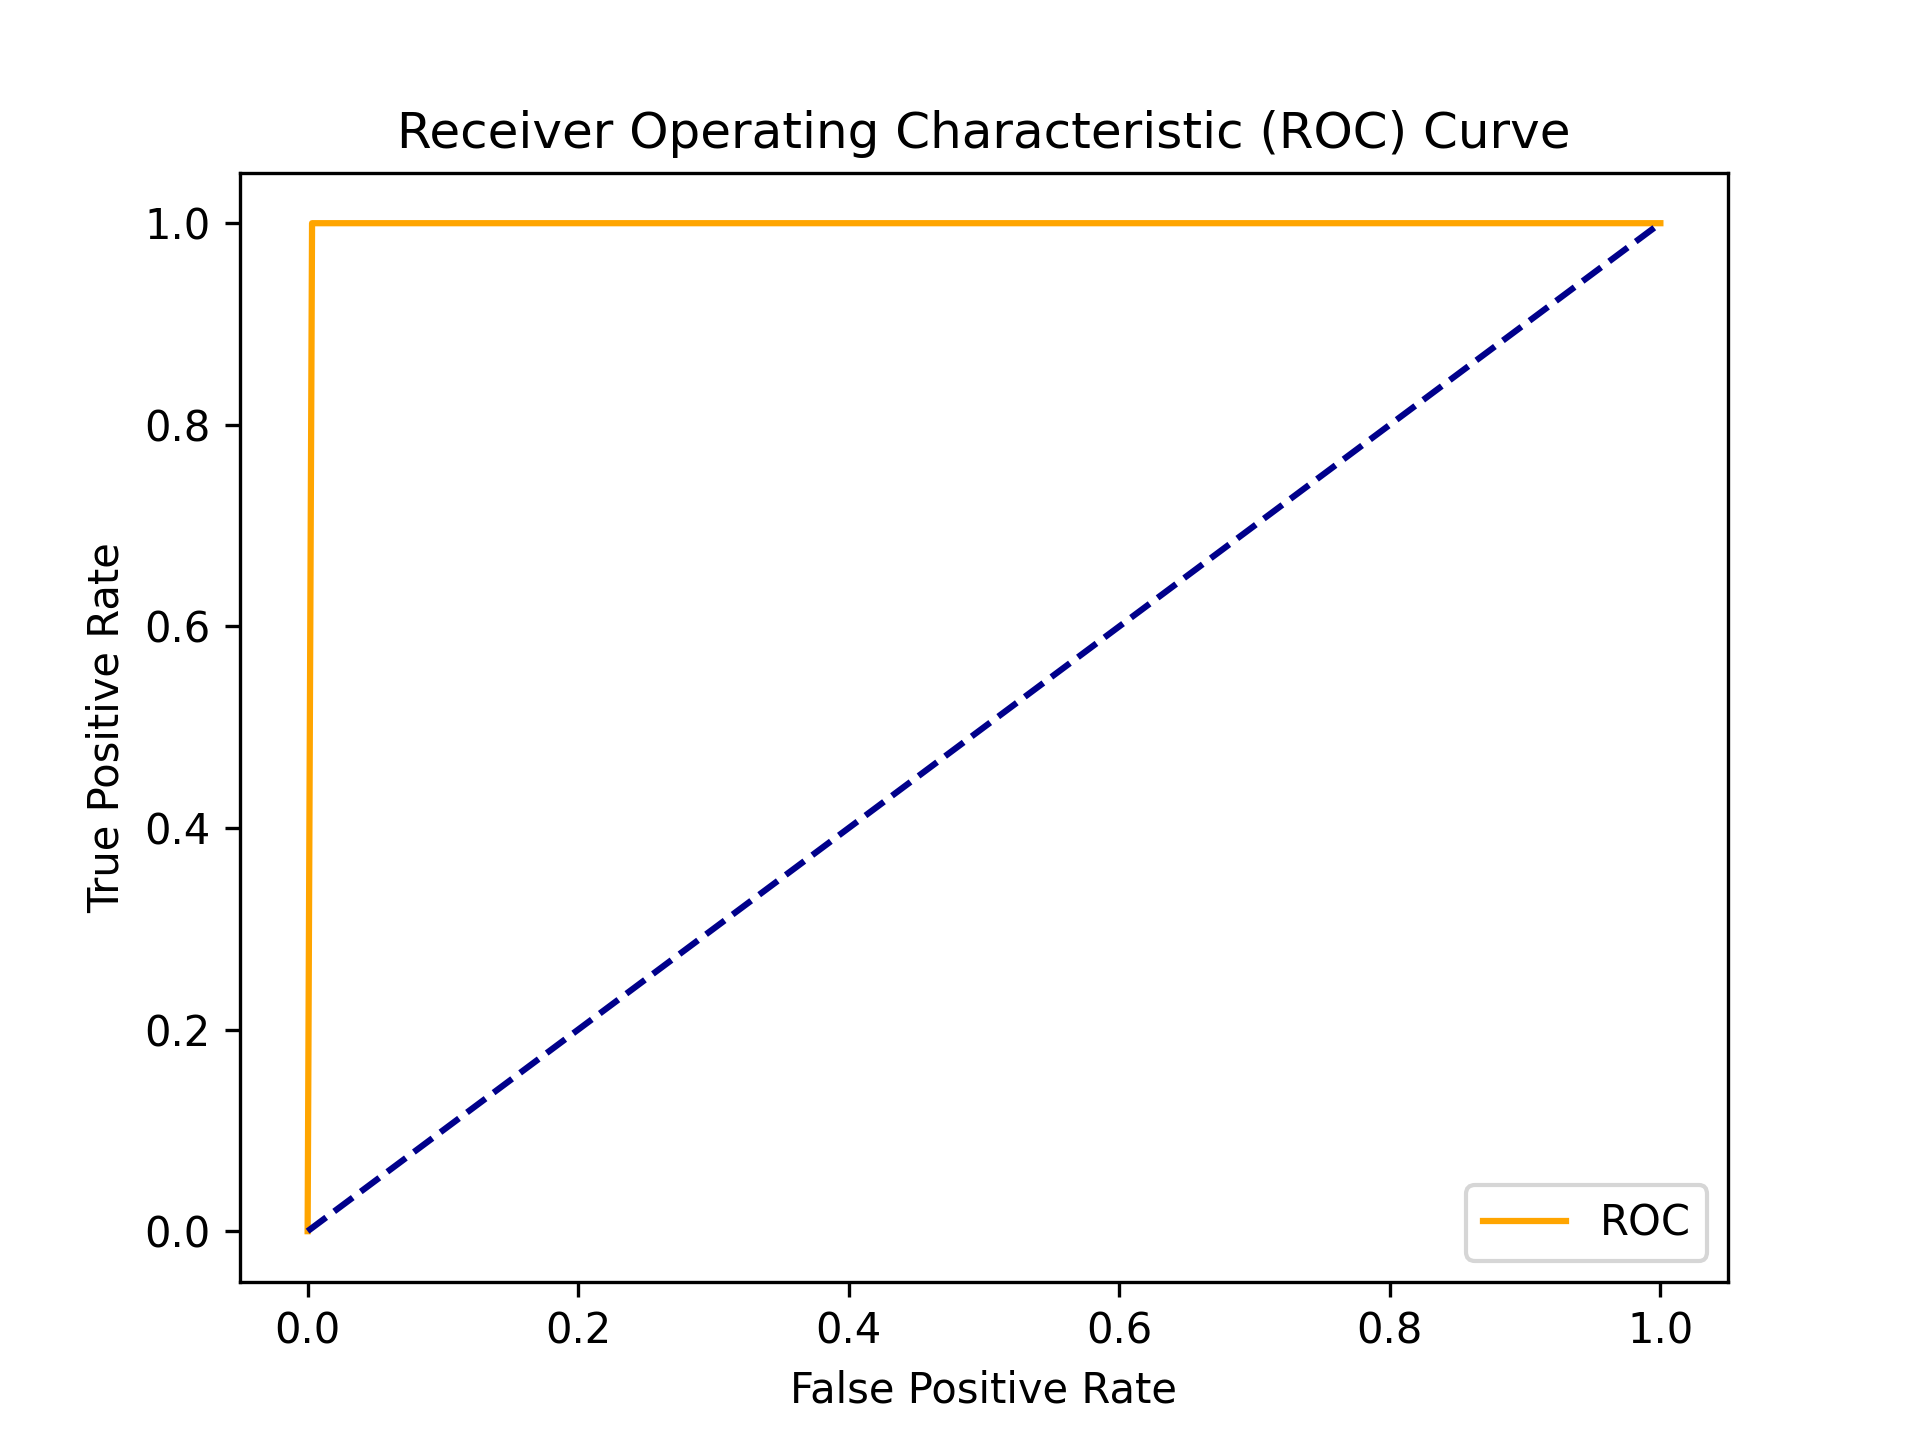
\includegraphics[trim={1cm 0.5cm 0cm 1cm}, width=0.322\textwidth]{results/transfer/roc_curve_transfer_regression_gpt_0.15.png}}
\hspace{\fill}
   \subfloat[XL\label{fig:roc_curve_xl_transfer_regression}]{%
      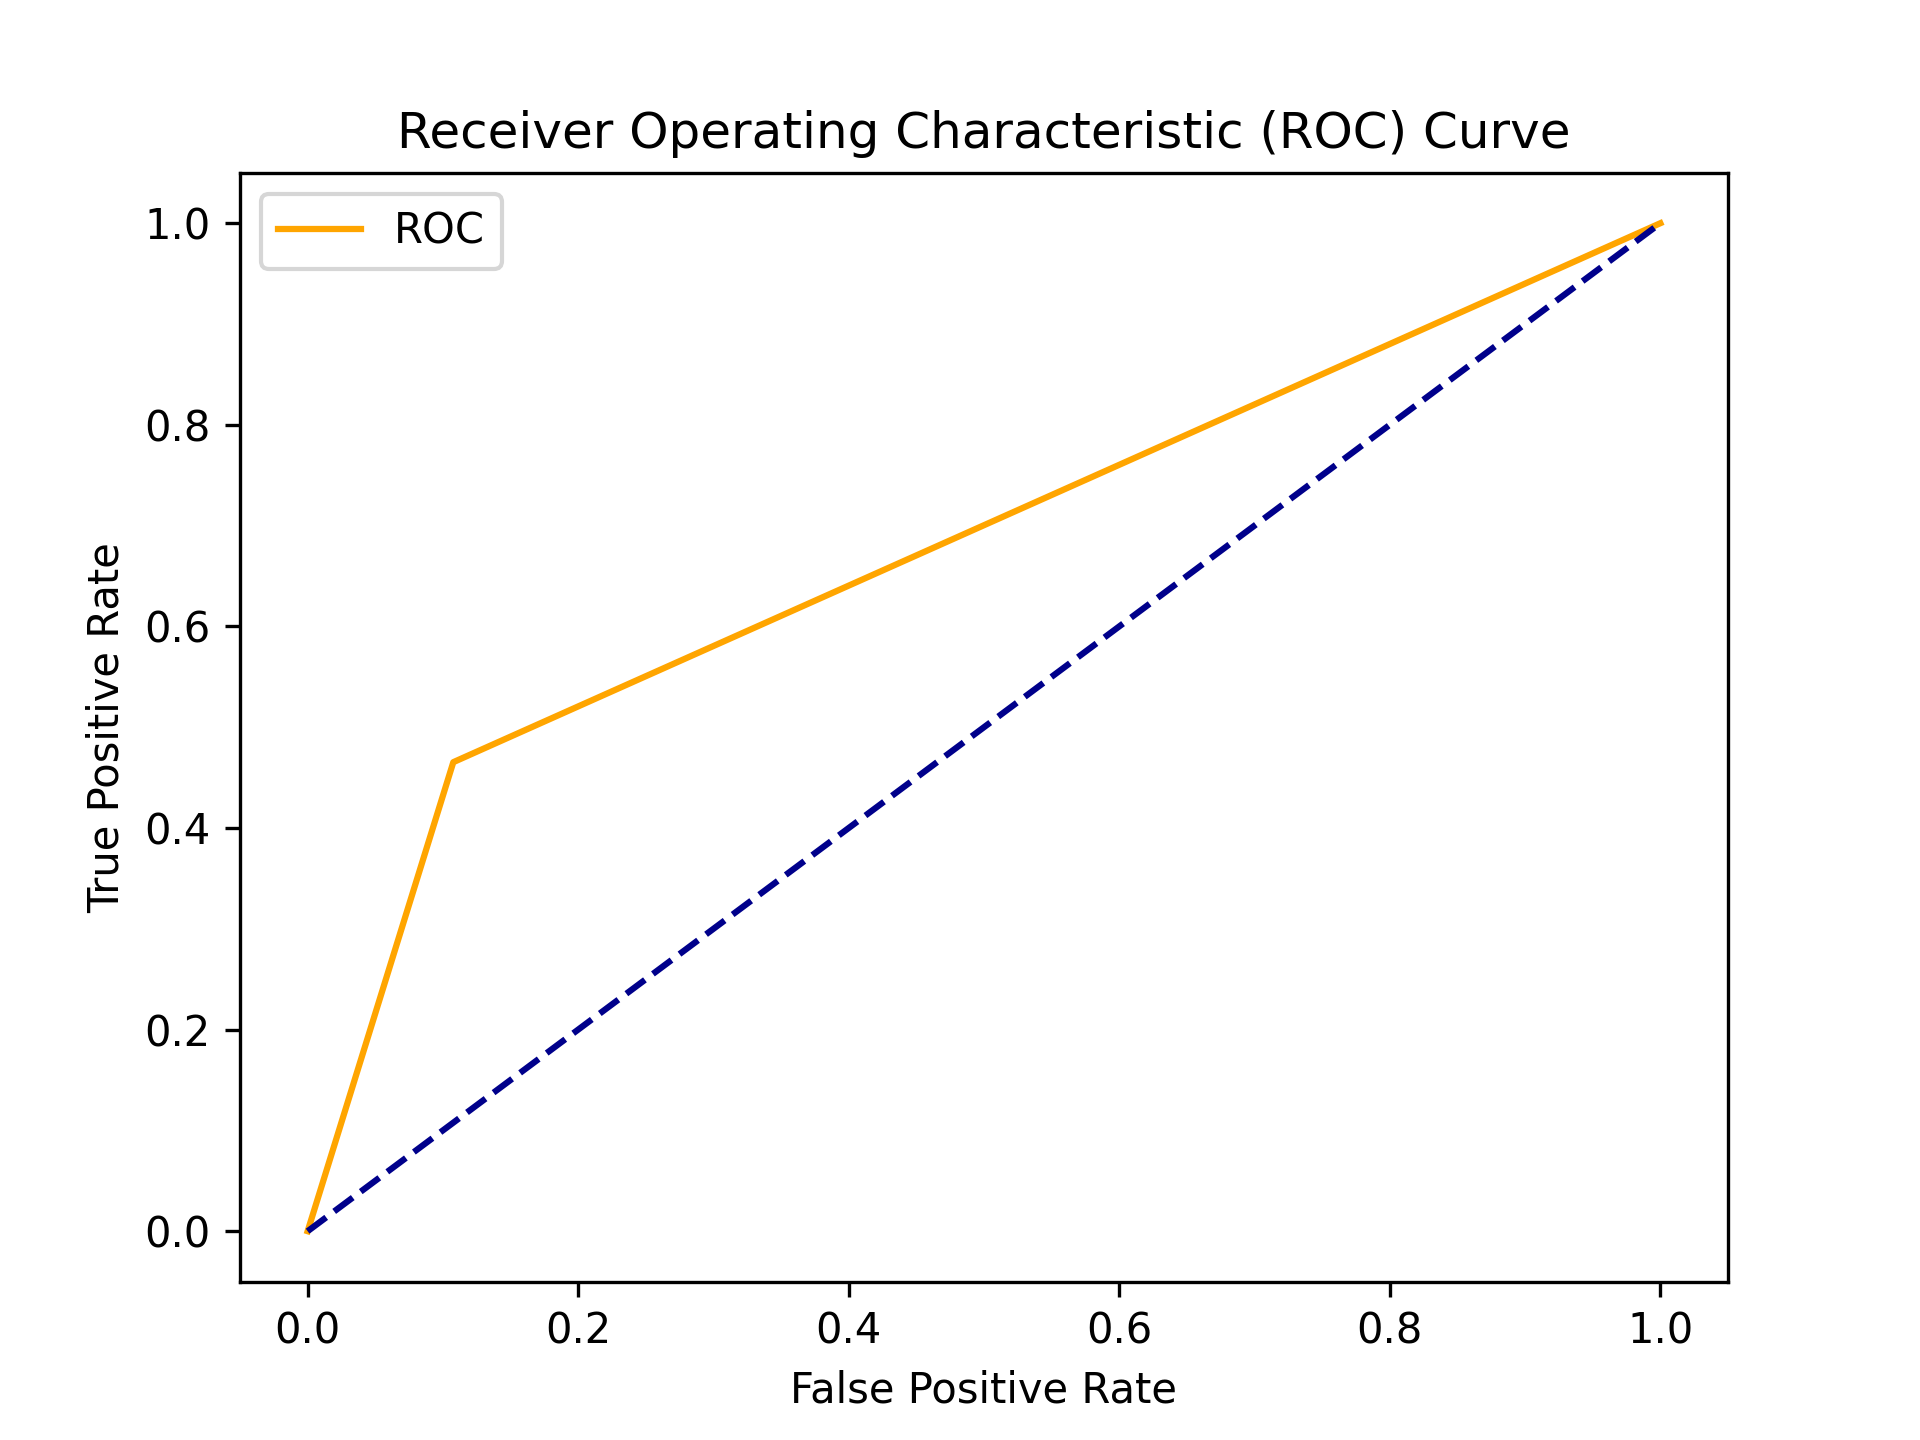
\includegraphics[trim={1cm 0.5cm 0cm 1cm}, width=0.322\textwidth]{results/transfer/roc_curve_transfer_regression_xl_0.15.png}}\\
\caption{\label{fig:results_transfer_regression_roc}ROC-Curve for transfer of knowledge using regression with 15\% alterations.}
\end{figure*}
%\end{comment}

\begin{figure}[H]
  \centering
  \captionsetup{justification=centering}
  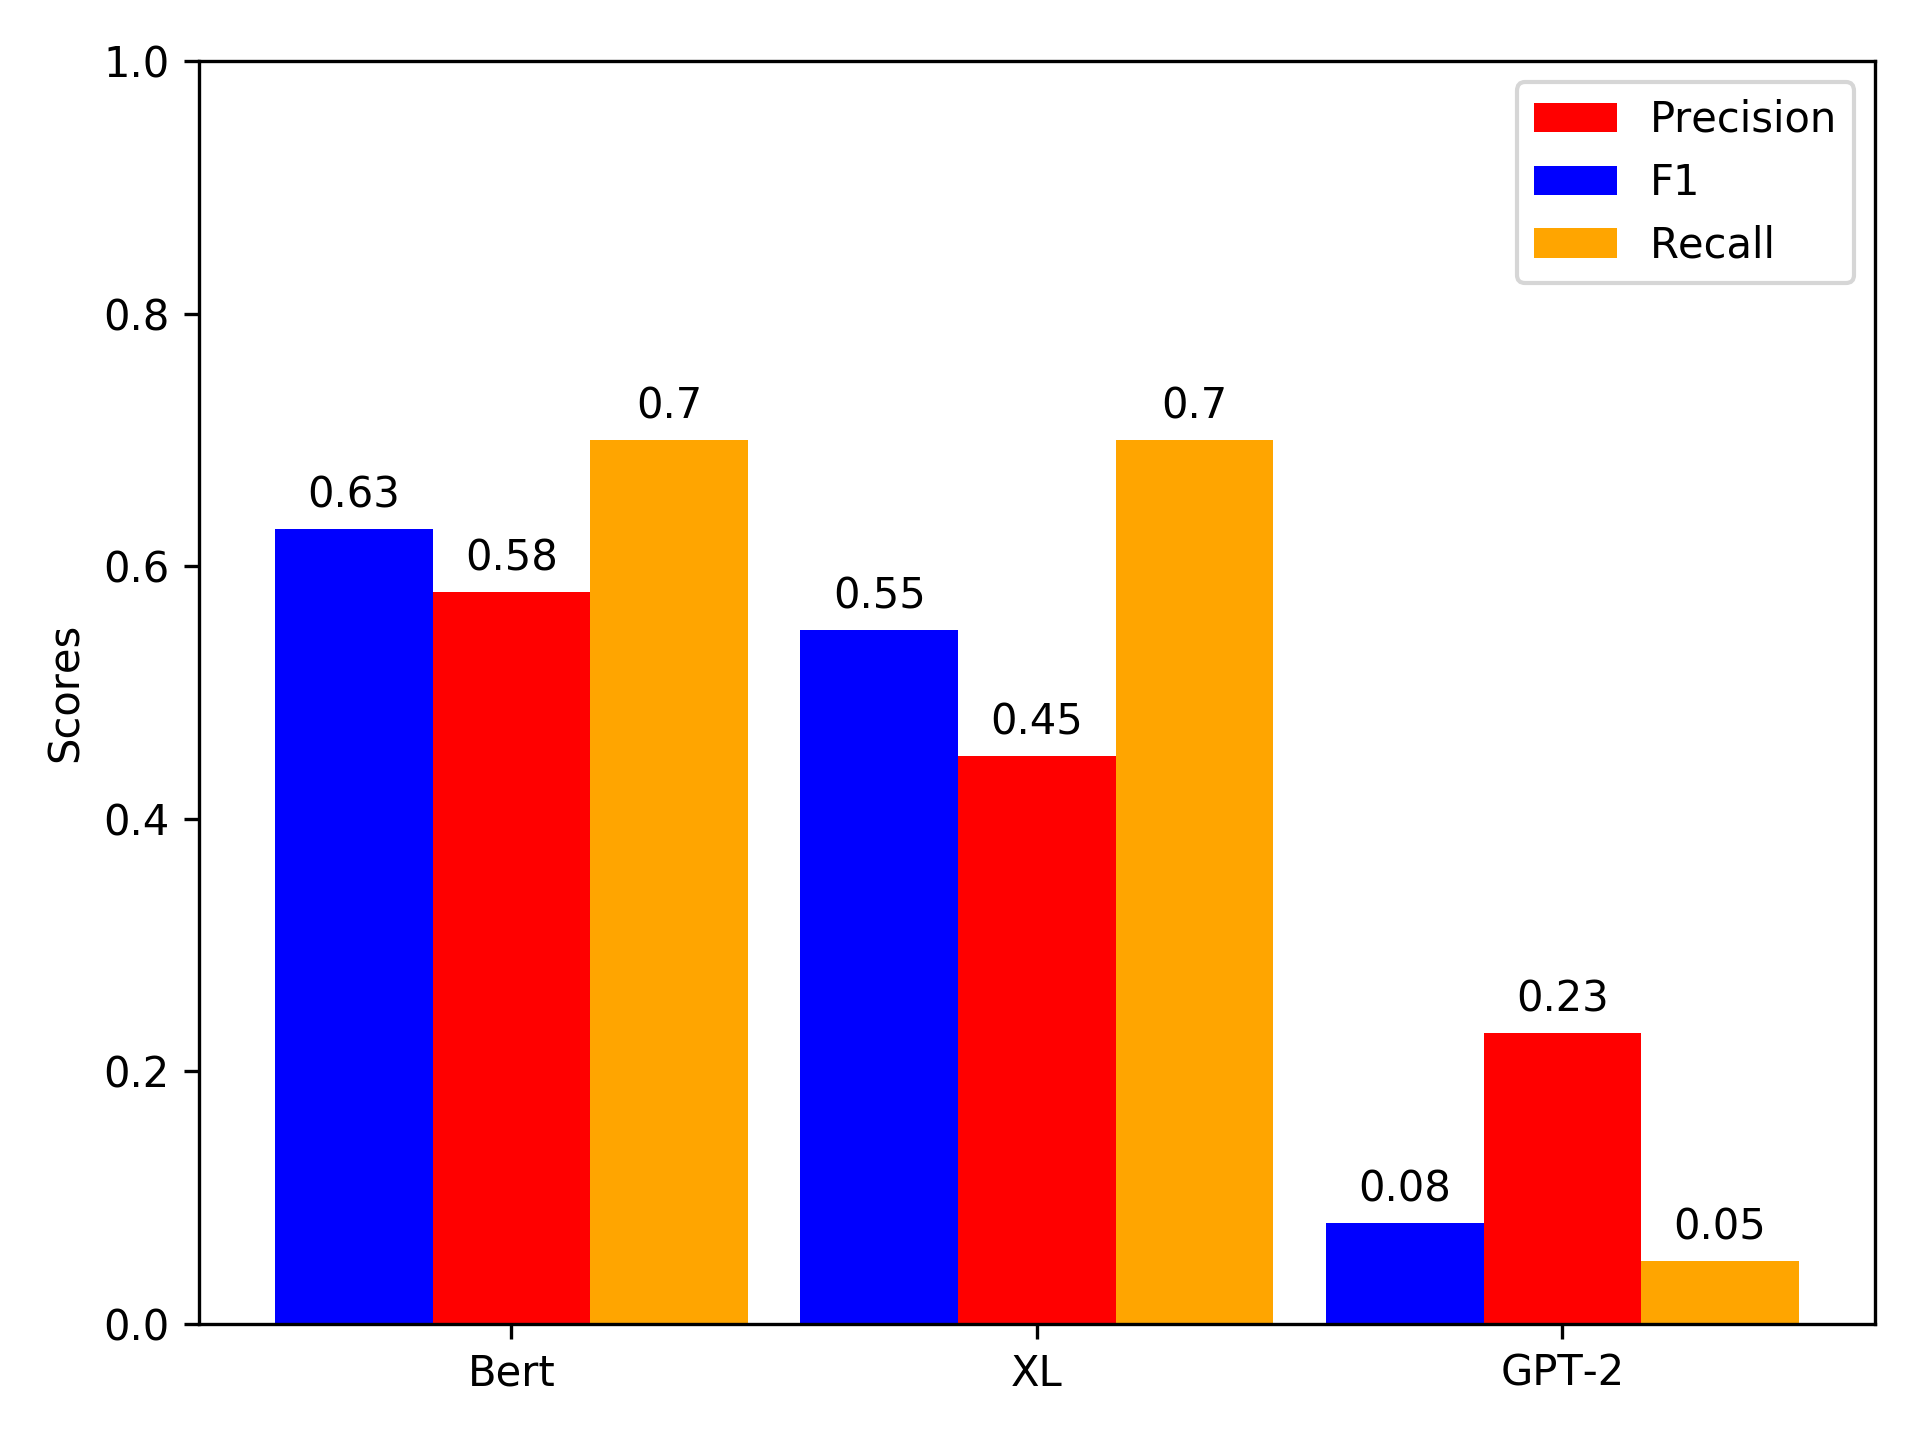
\includegraphics[width=8cm]{results/transfer_regression_replace_half.png}\\
  \caption{Transfer of knowledge. For 15\% of lines, replace 50\% of words, mark as anomaly, using regression.}
  \label{fig:replace_words_regression_transfer}
\end{figure}

%%%% TRANSFER LEARNING CLASSIFICATION
\subsection{Transfer of knowledge using the classification-based approach \label{sec:results-classification-transfer}}

For transfer of knowledge using the classification-based approach, the same experiments as described in \ref{sec:results-regression-transfer} were conducted. Figure \ref{fig:results_transfer_classification} shows the results of the transfer of knowledge experiment. Interesting observations include the stable results achieved using Bert, which are little sensitive to increasing alteration ratios. Bert achieves a F1-score of 0.82 for 5\% alterations, 0.77 for 10\% alterations and 0.81 for 15\% alterations, and precision of 0.7 for 5\% alterations, 0.63 for 10\% alterations and 0.68 for 15\% alterations. For XL-Transformers, the F1-score is 0.46 for 5\% alterations, 0.61 for 10\% alterations and 0.38 for 15\% alterations, while precision goes from 0.3 for 5\% alterations to 0.44 for 10\% alterations to 0.23 for 15\% alterations. GPT-2 shows overall far worse results than for regression, with only 0.17 F1-score and 0.09 precision for 15\% alteration ratio.
These results show that Bert has clear advantages over GPT-2 and XL-Transformers for the classification-based approach. It is noticeable, that all language models achieve a recall value of 1.0. This is due to the high cosine distance of the injected anomaly log event in comparison to the other log events.
Figure \ref{fig:results_transfer_multiclass_per_epoch} depicts the development of the metrics of detecting anomalies for every additional epoch of training on dataset B. After every epoch of training on the train dataset B, the labelled test dataset B is fed into the model, and metrics are collected. Bert improves the most per epoch, ramping up steeply in accuracy and especially for F1-score and precision between epoch four and five. GPT-2 shows almost no improvements, with F1, precision and accuracy and XL-Transformers has small improvements over the course of the 5 epochs. These findings are confirmed by the ROC curve plots which can be seen in figure \ref{fig:results_transfer_multiclass_roc}, showing very good results for Bert, acceptable results for Xl-Transformers and far less satisfying results for GPT-2.

%\begin{figure}[h]
%  \centering
%  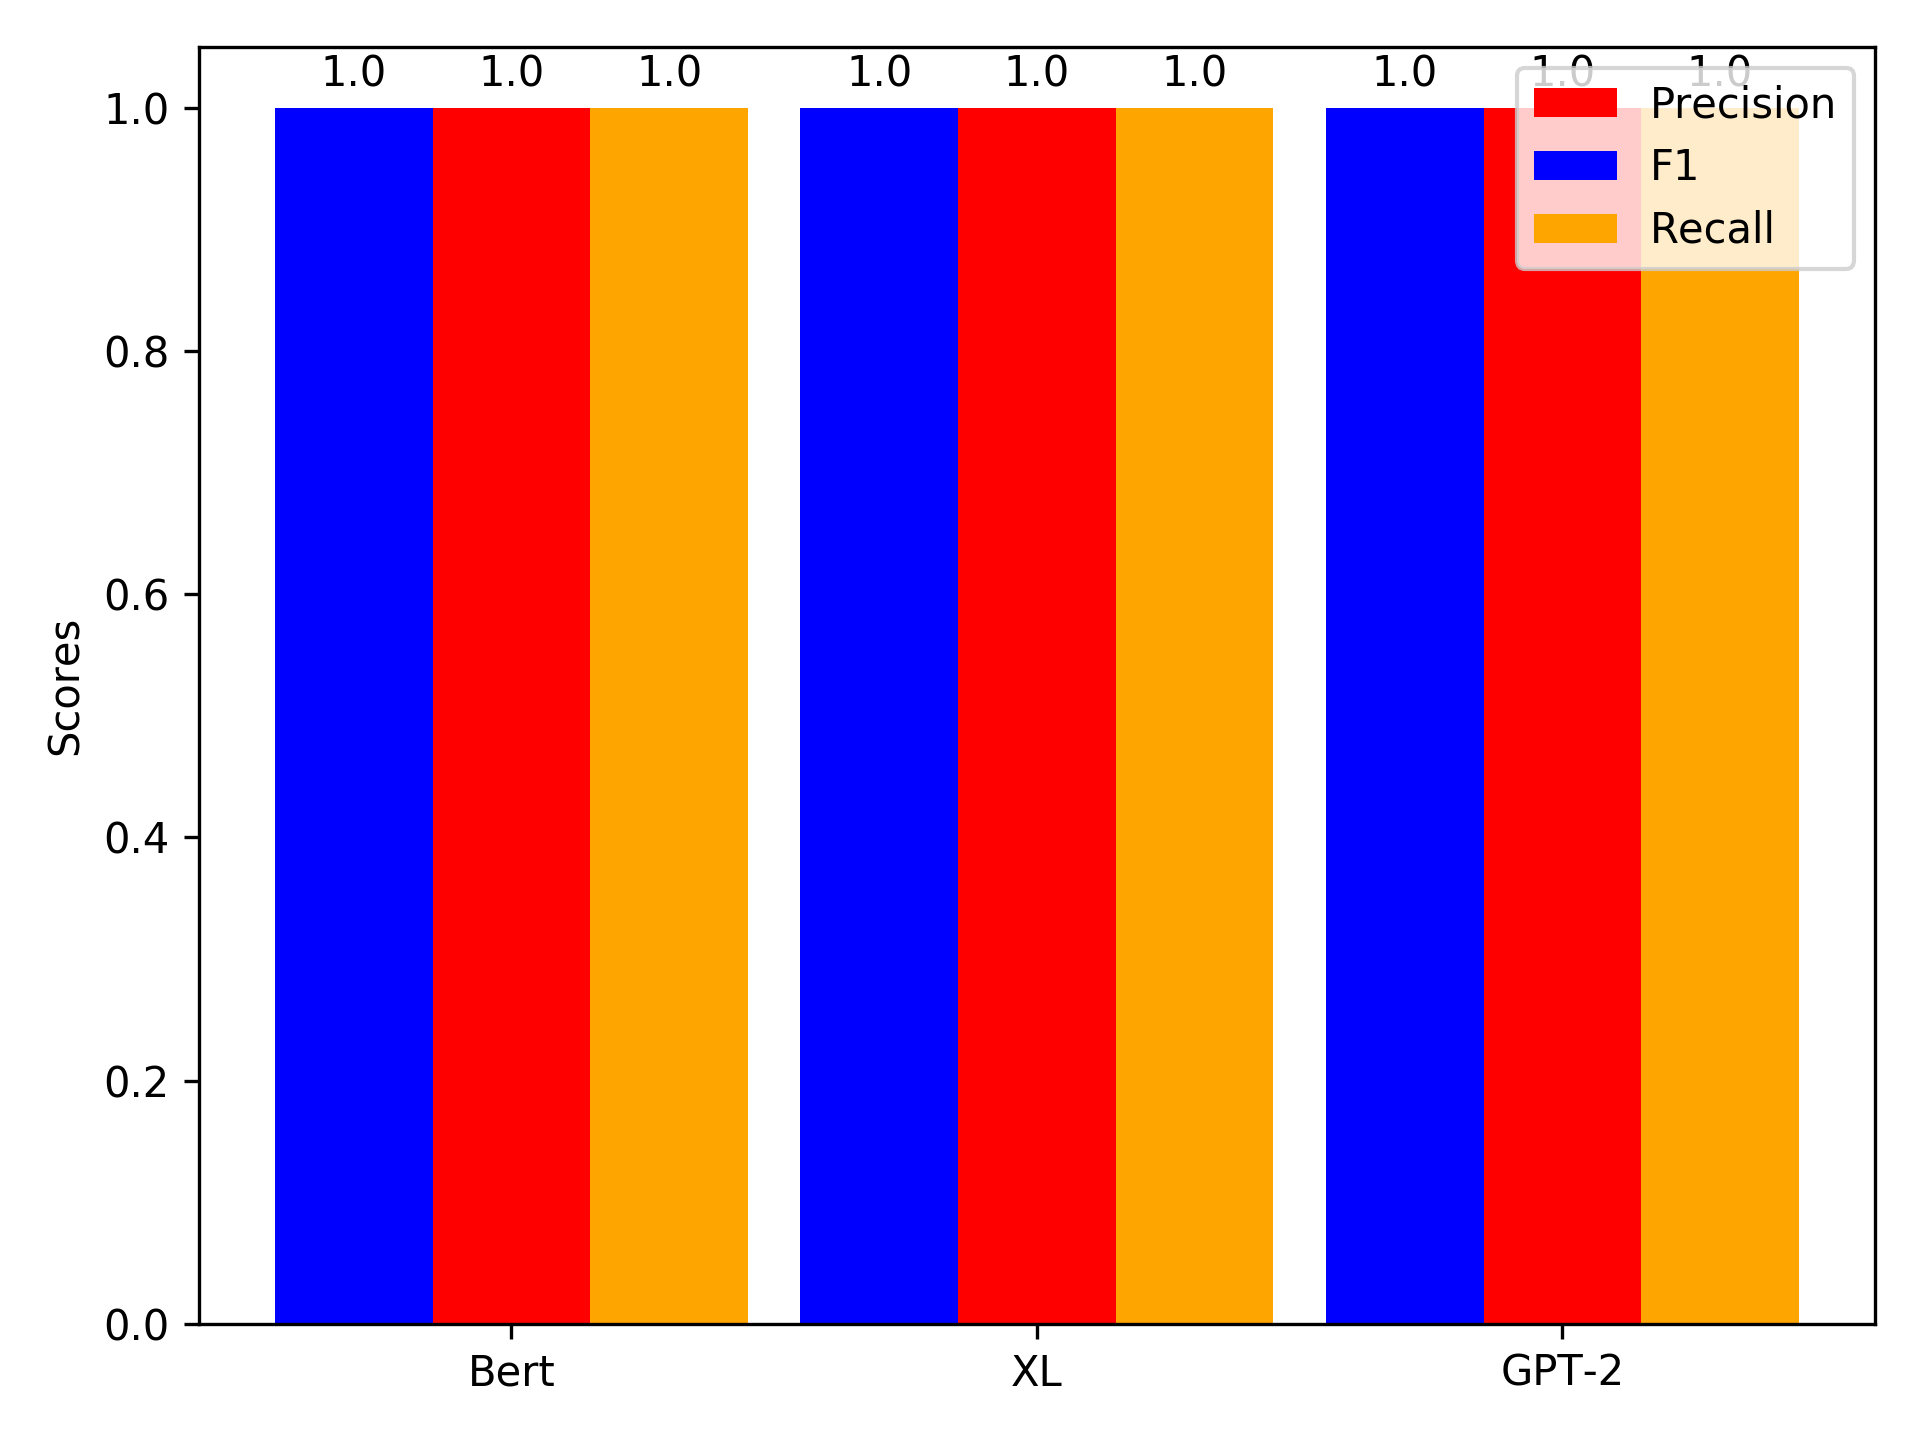
\includegraphics[width=6cm,height=4.5cm]{results/transfer/transfer_classification_reverse.png}\\
%  \caption{Scores for detecting reversed order of log events for transfer learning, using classification.}
%  \label{fig:classification_transfer_reverse}
  
%\end{figure}
\begin{figure*}[ht!]
\centering
  \captionsetup{justification=centering}
   \subfloat[5\% alteration\label{fig:results_transfer_classification_0.05}]{%
      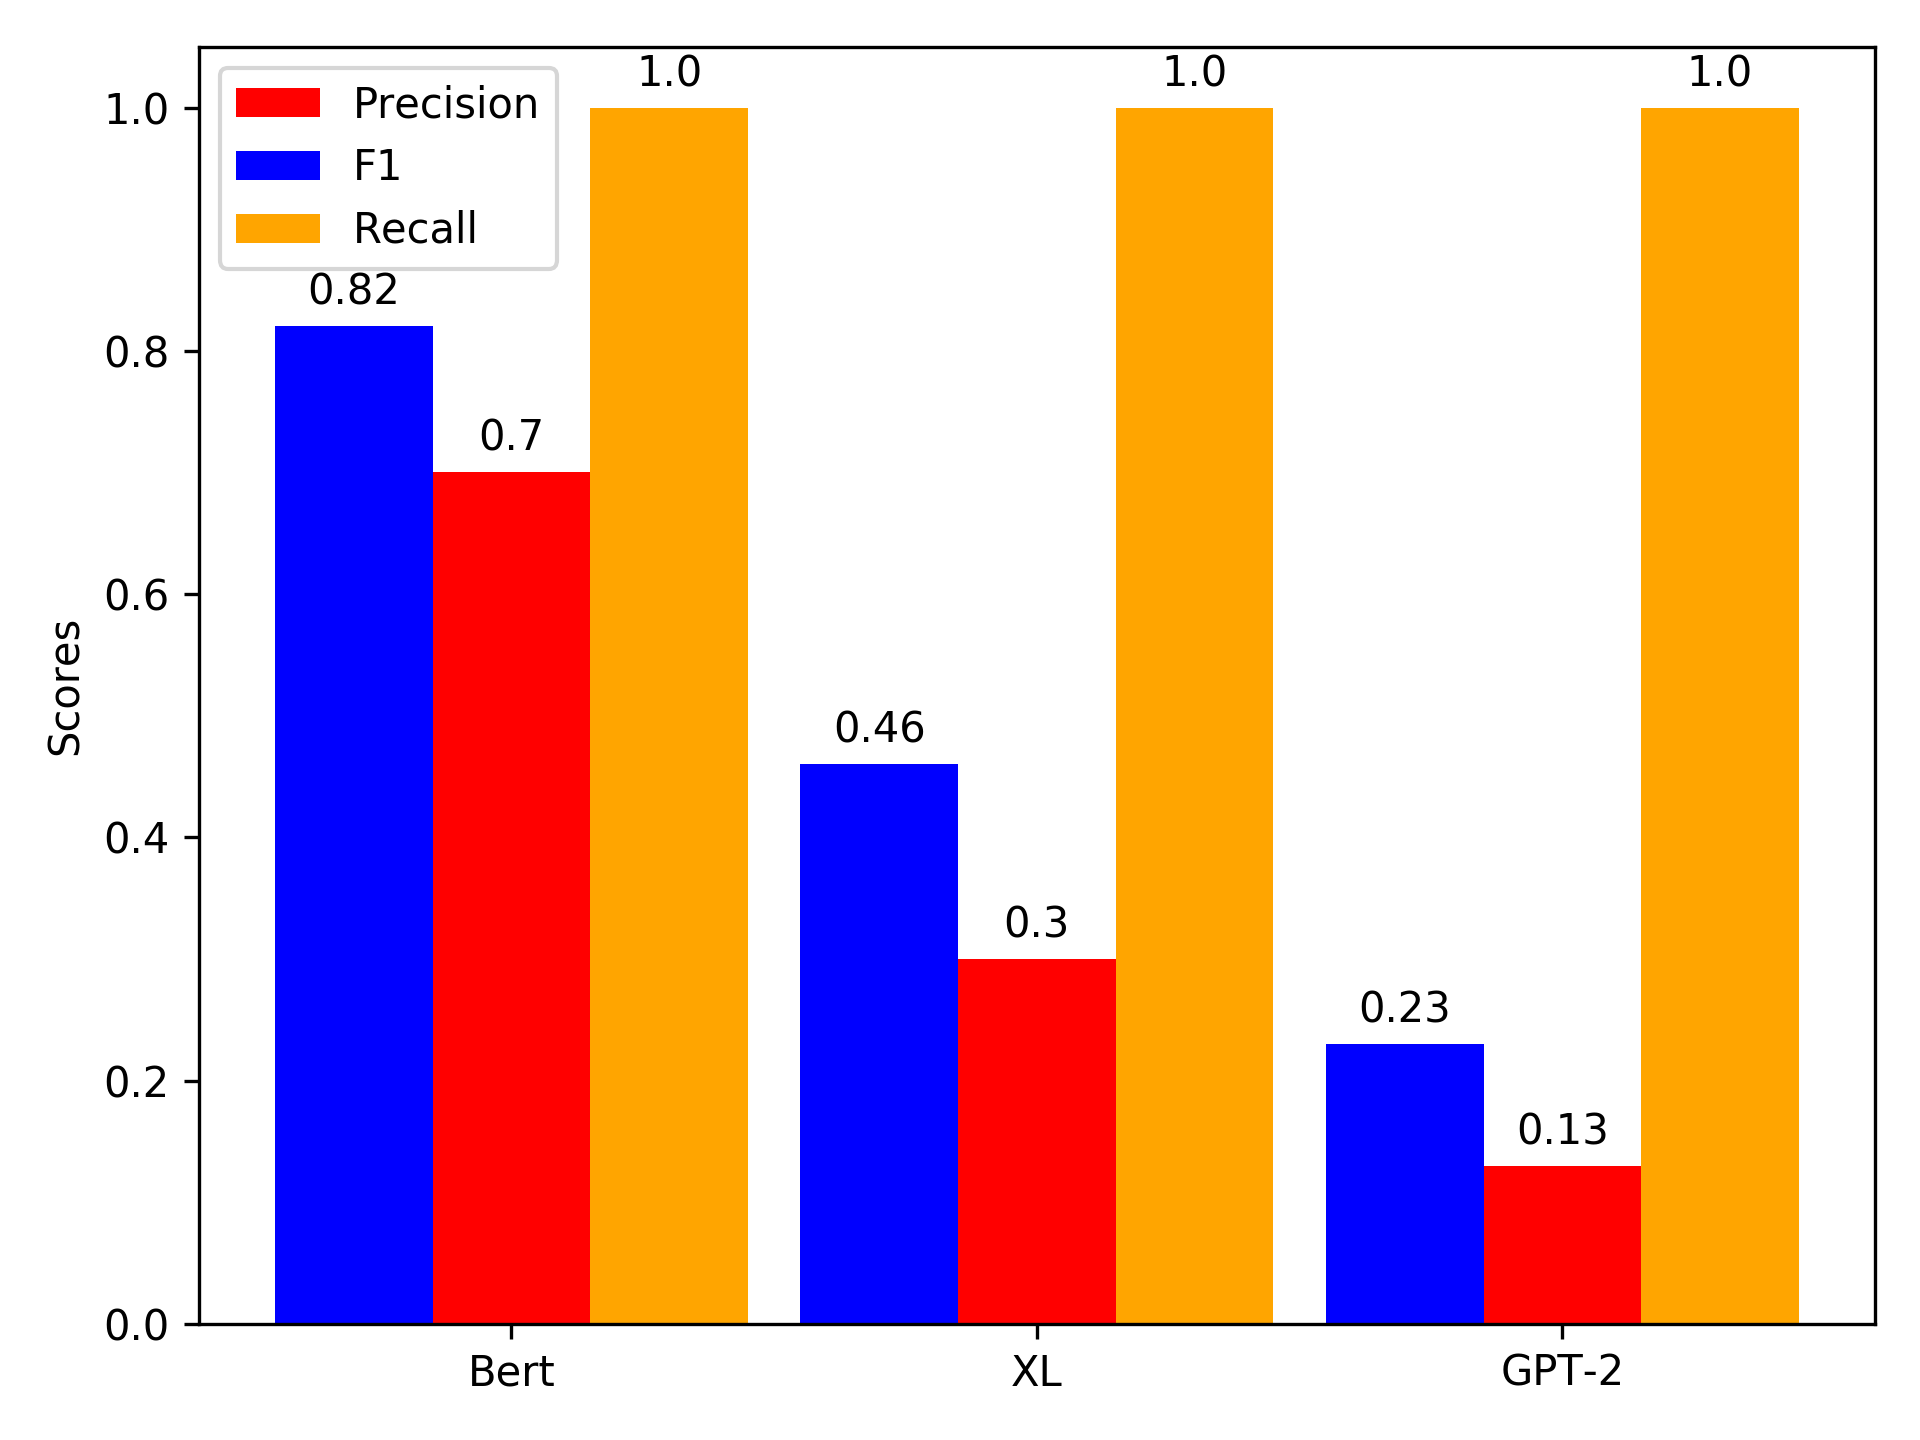
\includegraphics[trim={1cm 0.5cm 0cm 1cm}, width=0.322\textwidth]{results/transfer/transfer_multiclass_0.05_ratio.png}}
\hspace{\fill}
   \subfloat[10\% alteration\label{fig:results_transfer_classification_0.10} ]{%
      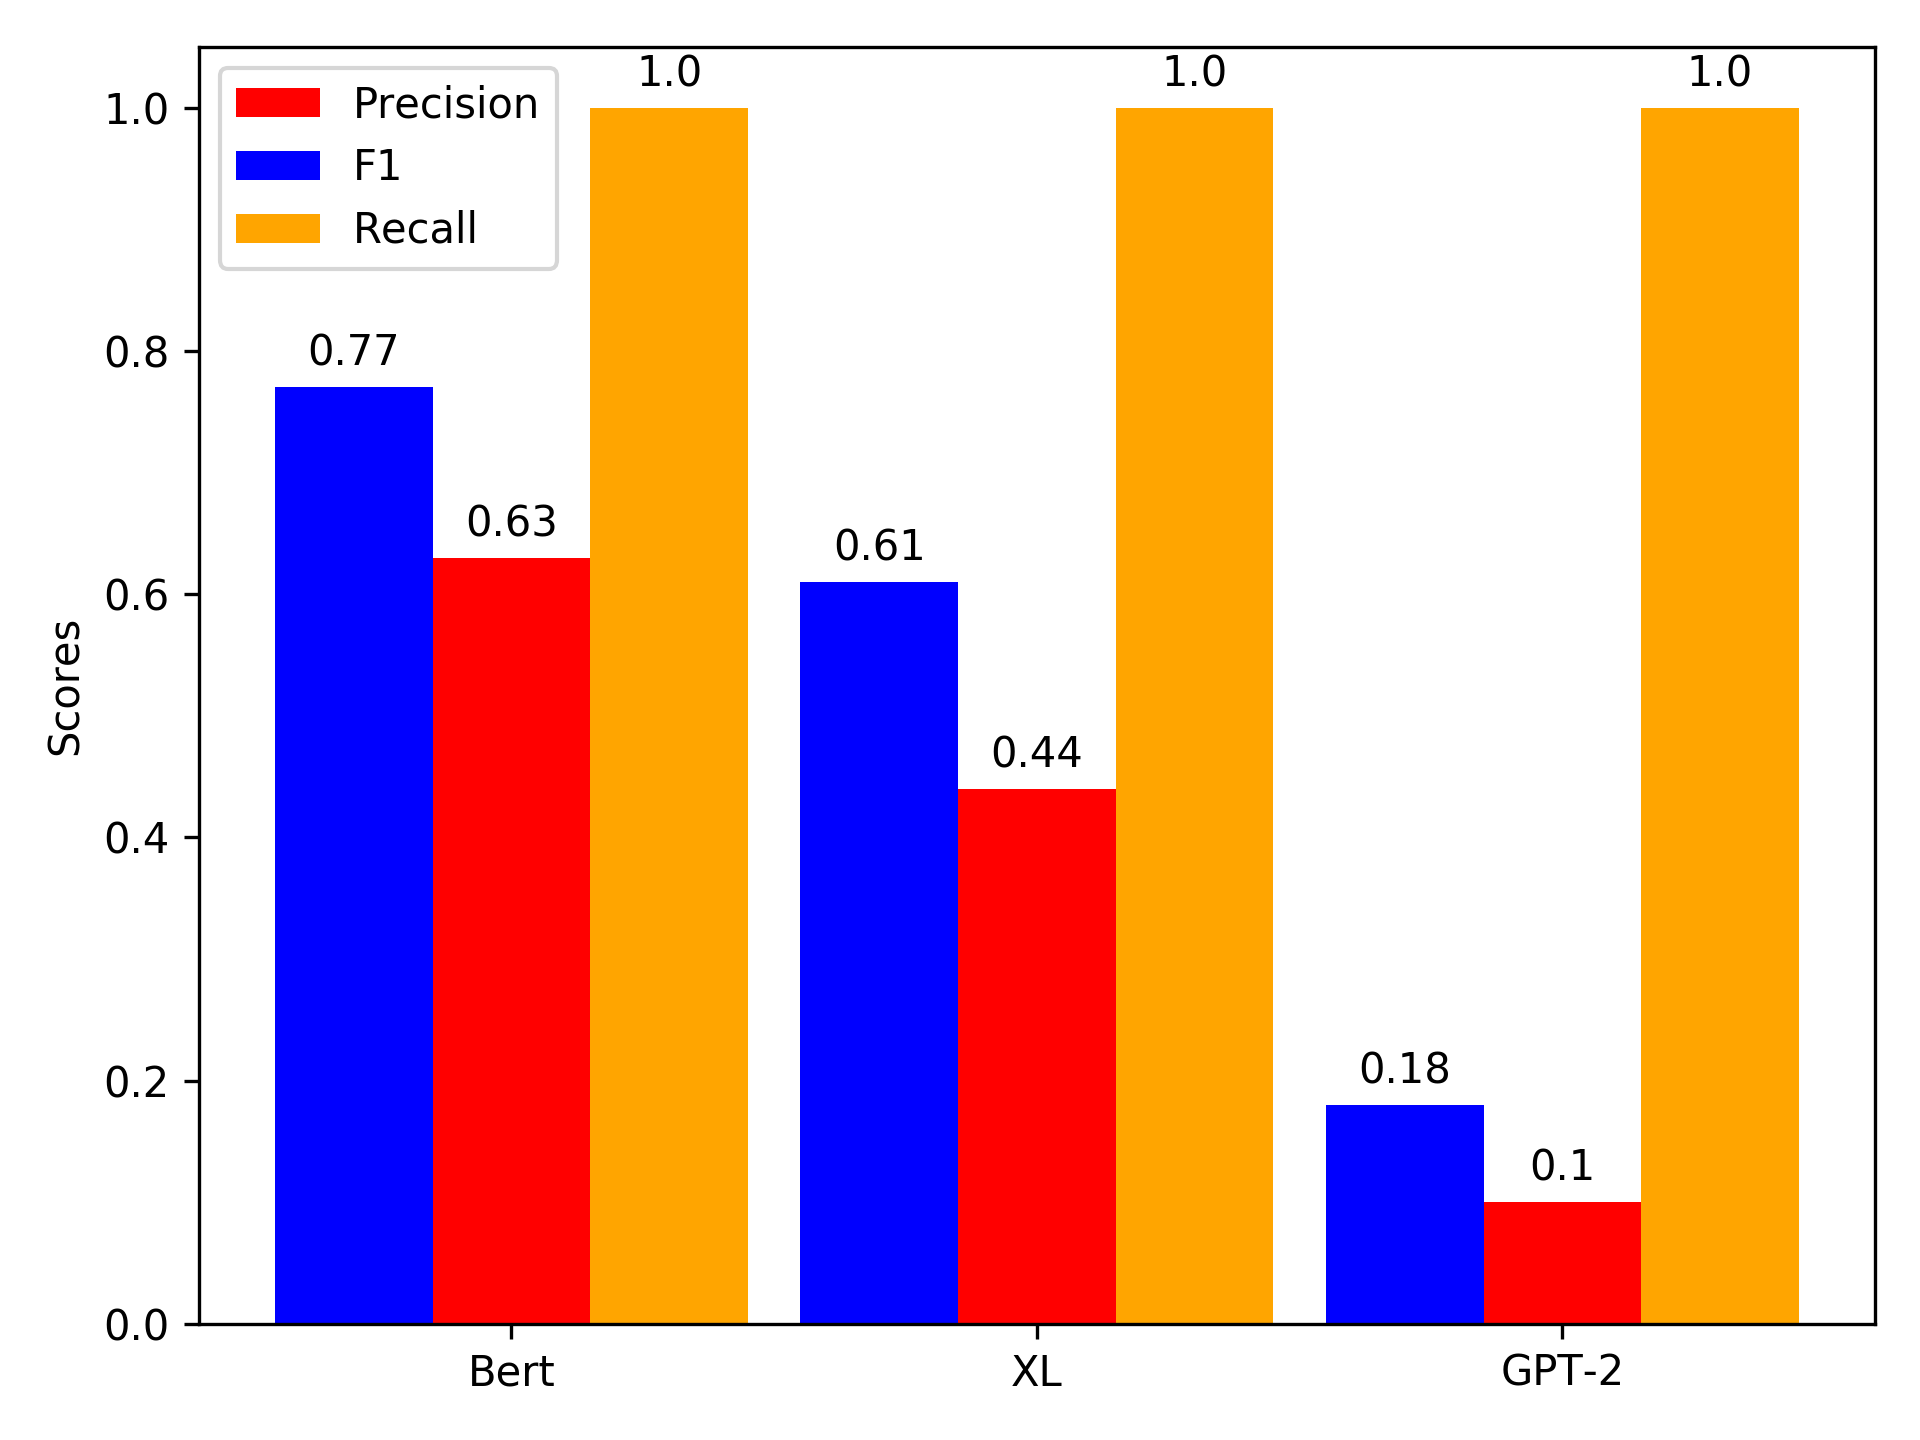
\includegraphics[trim={1cm 0.5cm 0cm 1cm}, width=0.322\textwidth]{results/transfer/transfer_multiclass_0.1_ratio.png}}
\hspace{\fill}
   \subfloat[15\% alteration\label{fig:results_transfer_classification_0.15}]{%
      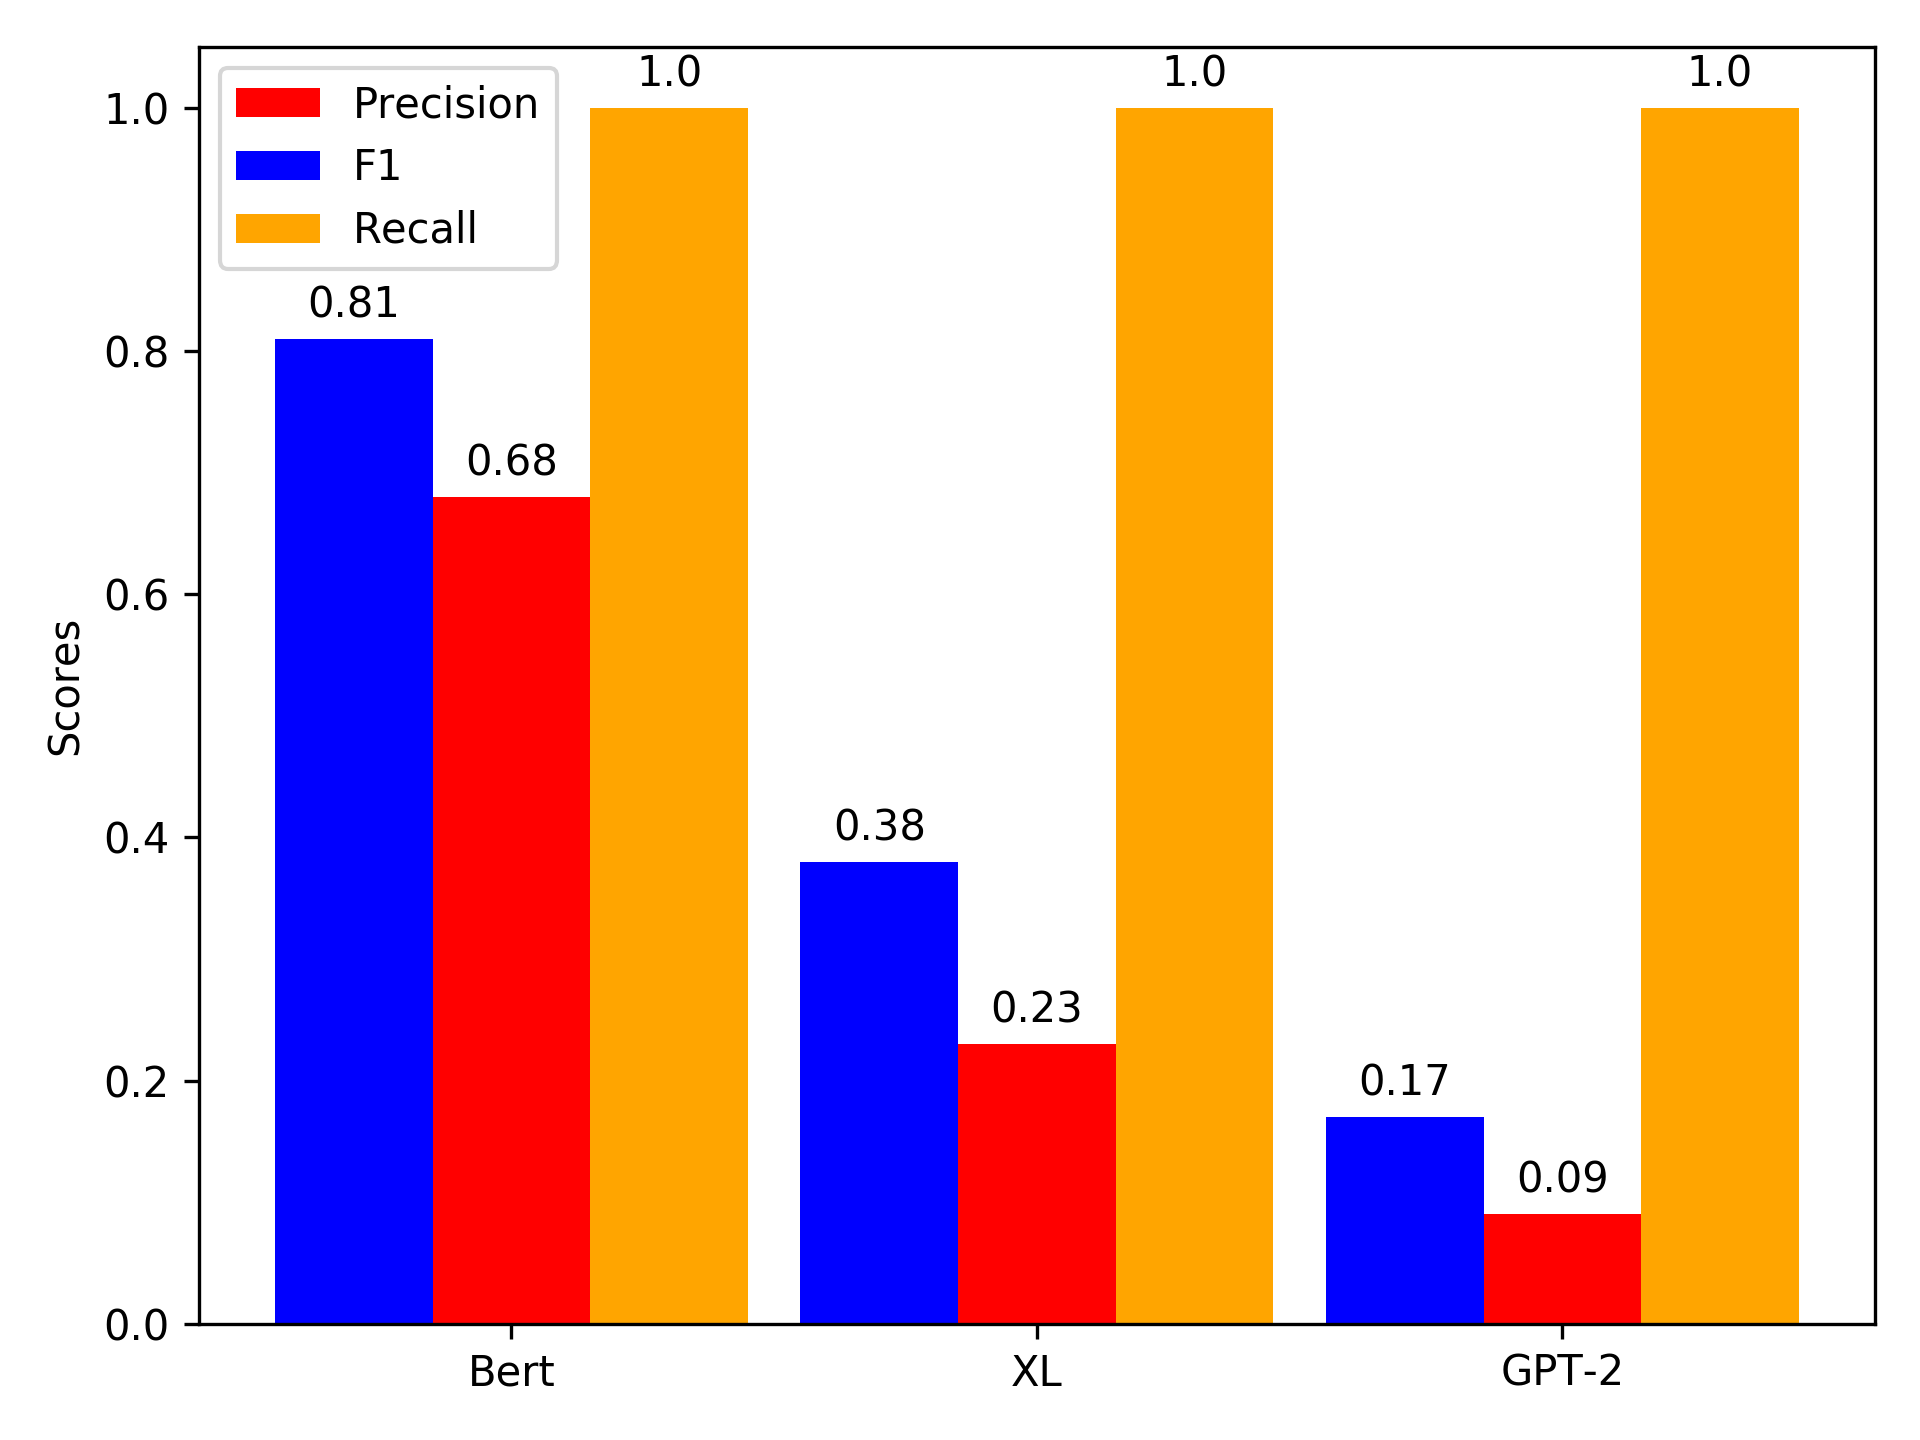
\includegraphics[trim={1cm 0.5cm 0cm 1cm}, width=0.322\textwidth]{results/transfer/transfer_multiclass_0.15_ratio.png}}\\
\caption{\label{fig:results_transfer_classification}Transfer of knowledge with different ratios of alteration, 5\% anomalies, using classification.}
\end{figure*}

\begin{figure*}[ht!]
   \subfloat[Bert\label{fig:results_transfer_multiclass_per_epoch_0.05}]{%
      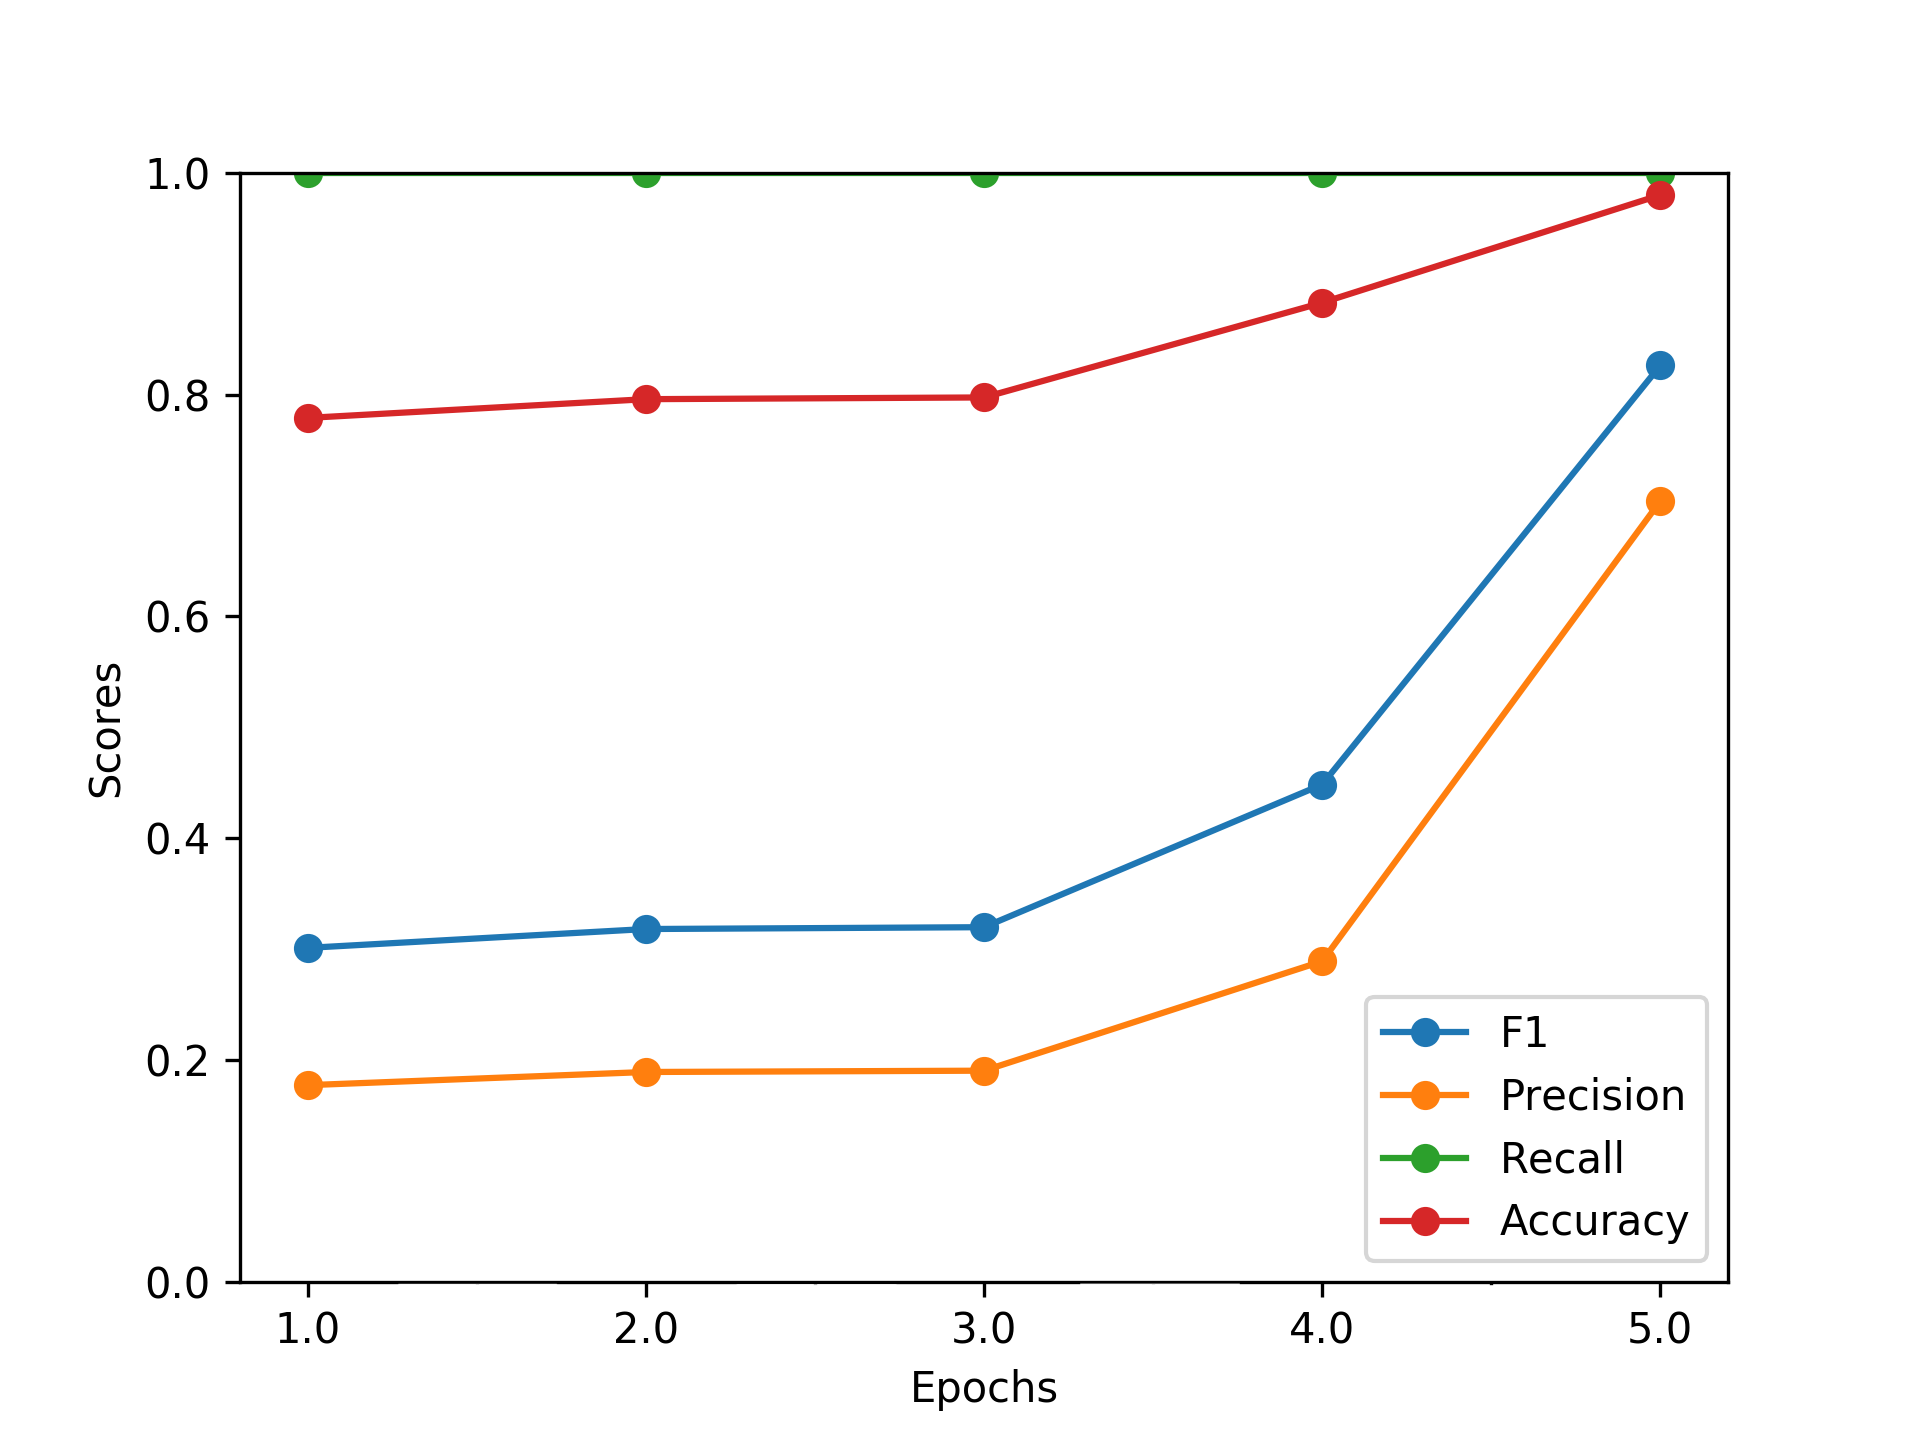
\includegraphics[trim={1cm 0.5cm 0cm 1cm}, width=0.322\textwidth]{results/transfer/bert_multiclass_0.15_transfer_metrics_per_epoch.png}}
\hspace{\fill}
   \subfloat[GPT-2\label{fig:results_transfer_multiclass_per_epoch_0.10} ]{%
      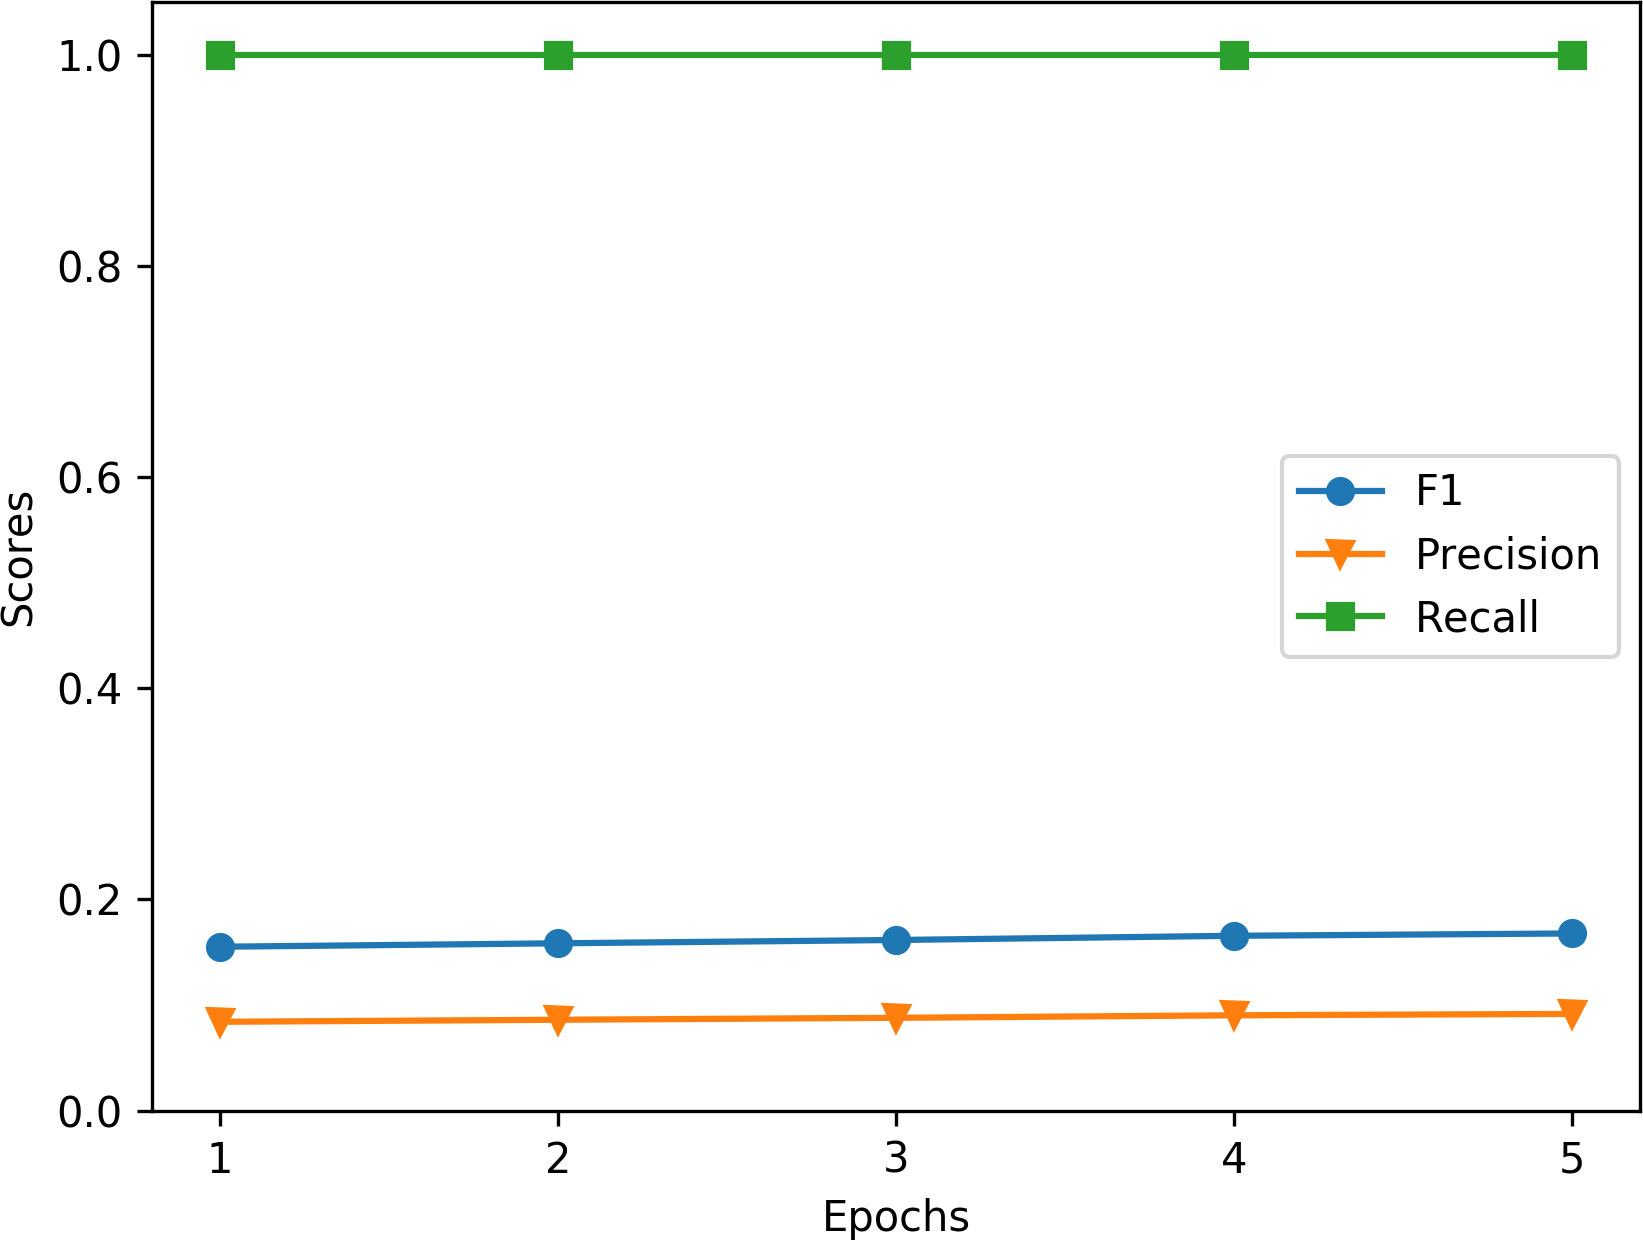
\includegraphics[trim={1cm 0.5cm 0cm 1cm}, width=0.322\textwidth]{results/transfer/gpt_multiclass_0.15_transfer_metrics_per_epoch.png}}
\hspace{\fill}
   \subfloat[XL\label{fig:results_transfer_multiclass_per_epoch_0.15}]{%
      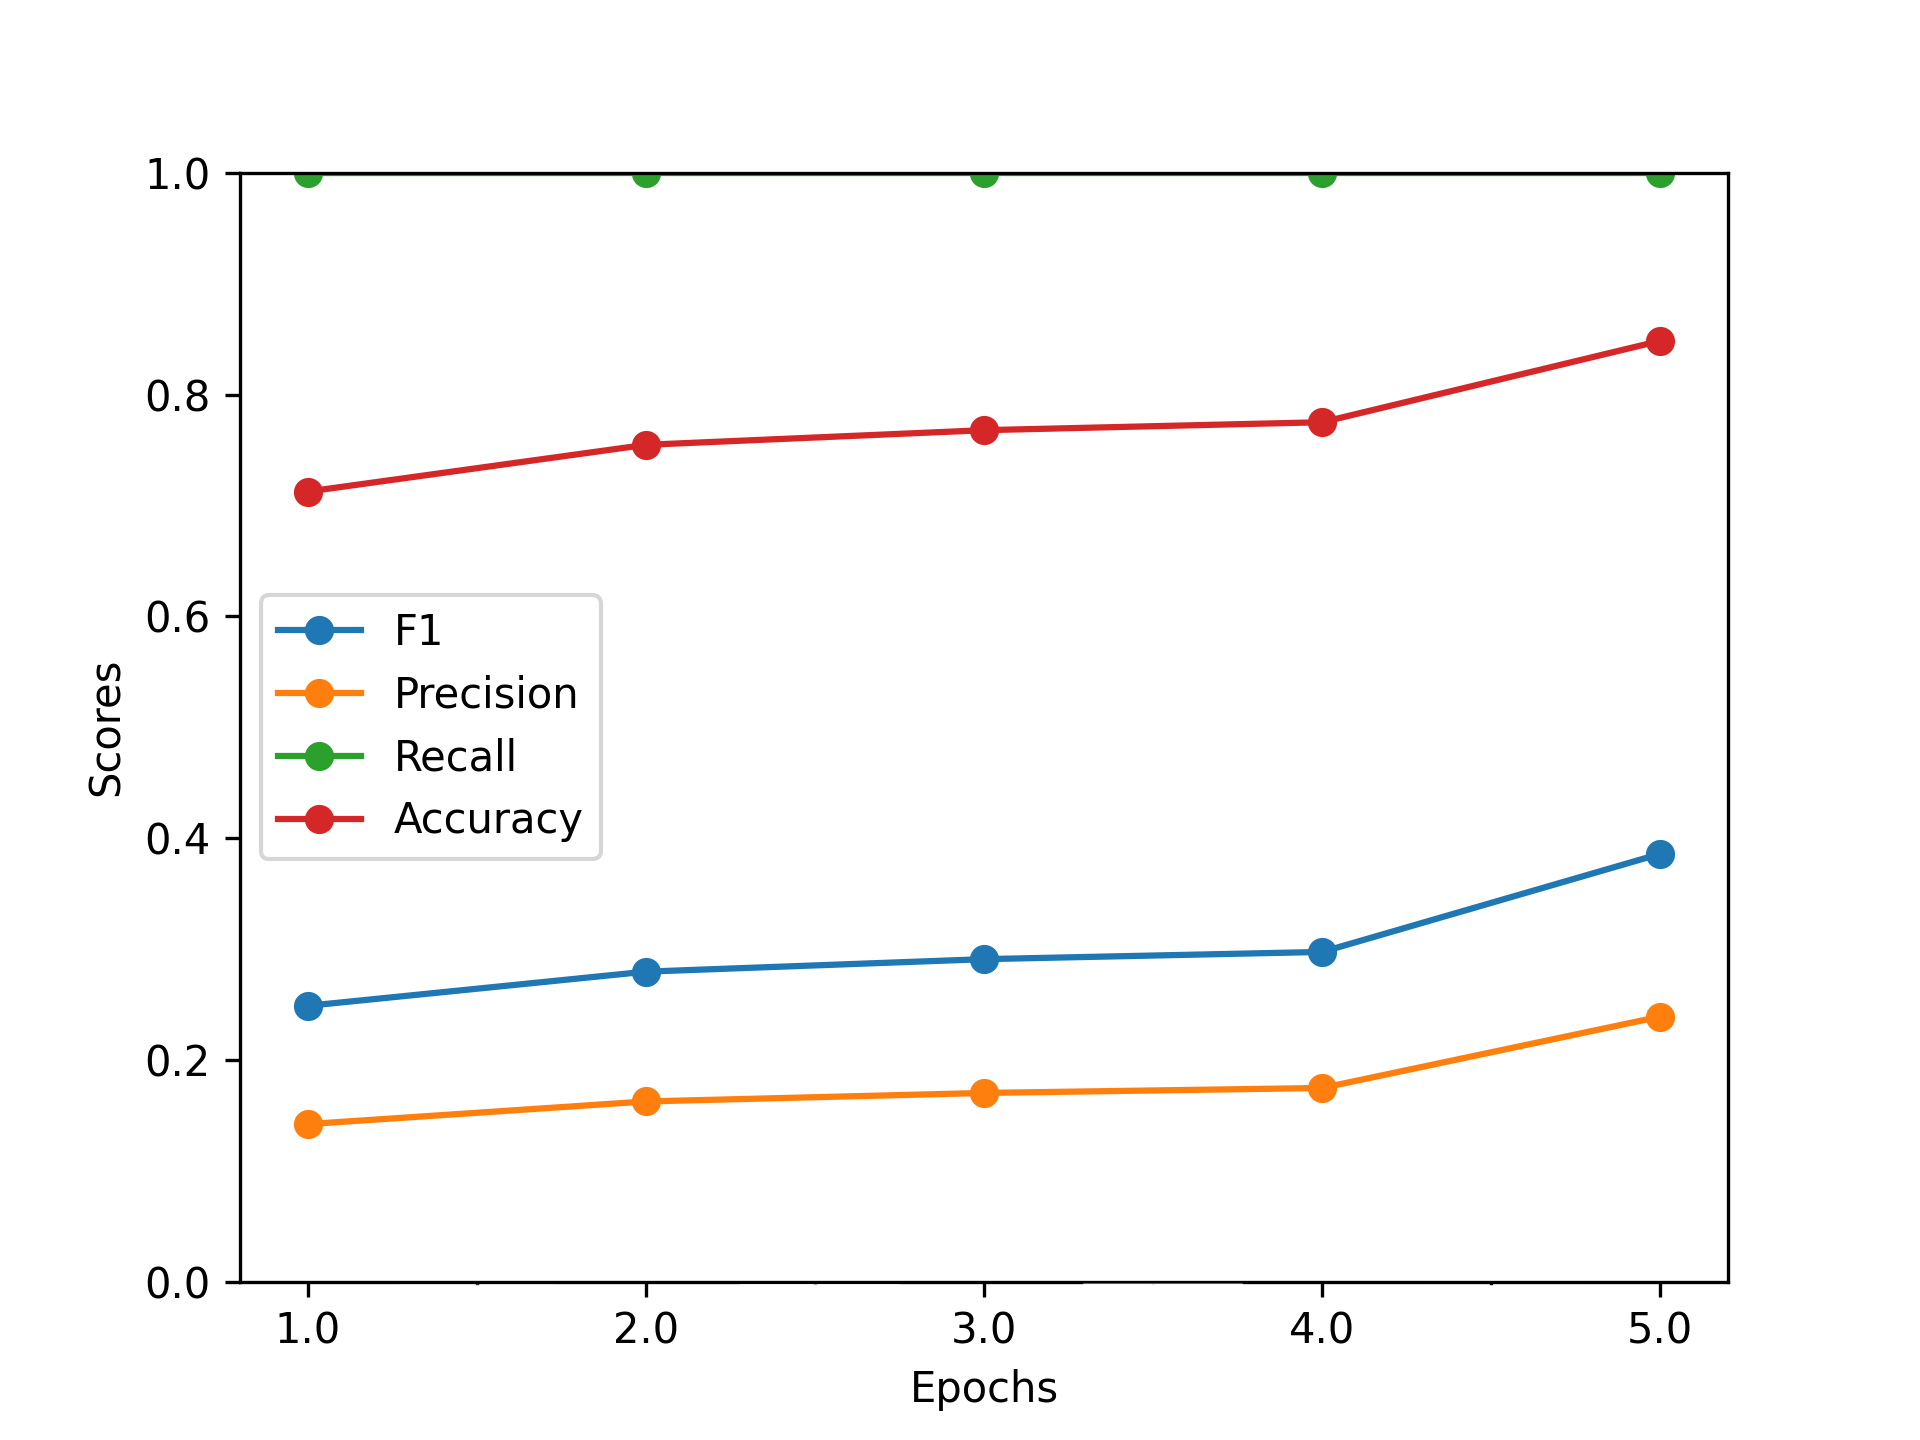
\includegraphics[trim={1cm 0.5cm 0cm 1cm}, width=0.322\textwidth]{results/transfer/xl_multiclass_0.15_transfer_metrics_per_epoch.png}}\\
\caption{\label{fig:results_transfer_multiclass_per_epoch}Improvement of metrics for transfer of knowledge per additional learning epoch, using classification.}
\end{figure*}


\begin{figure*}[ht!]
   \subfloat[Bert\label{fig:roc_curve_bert_transfer_multiclass}]{%
      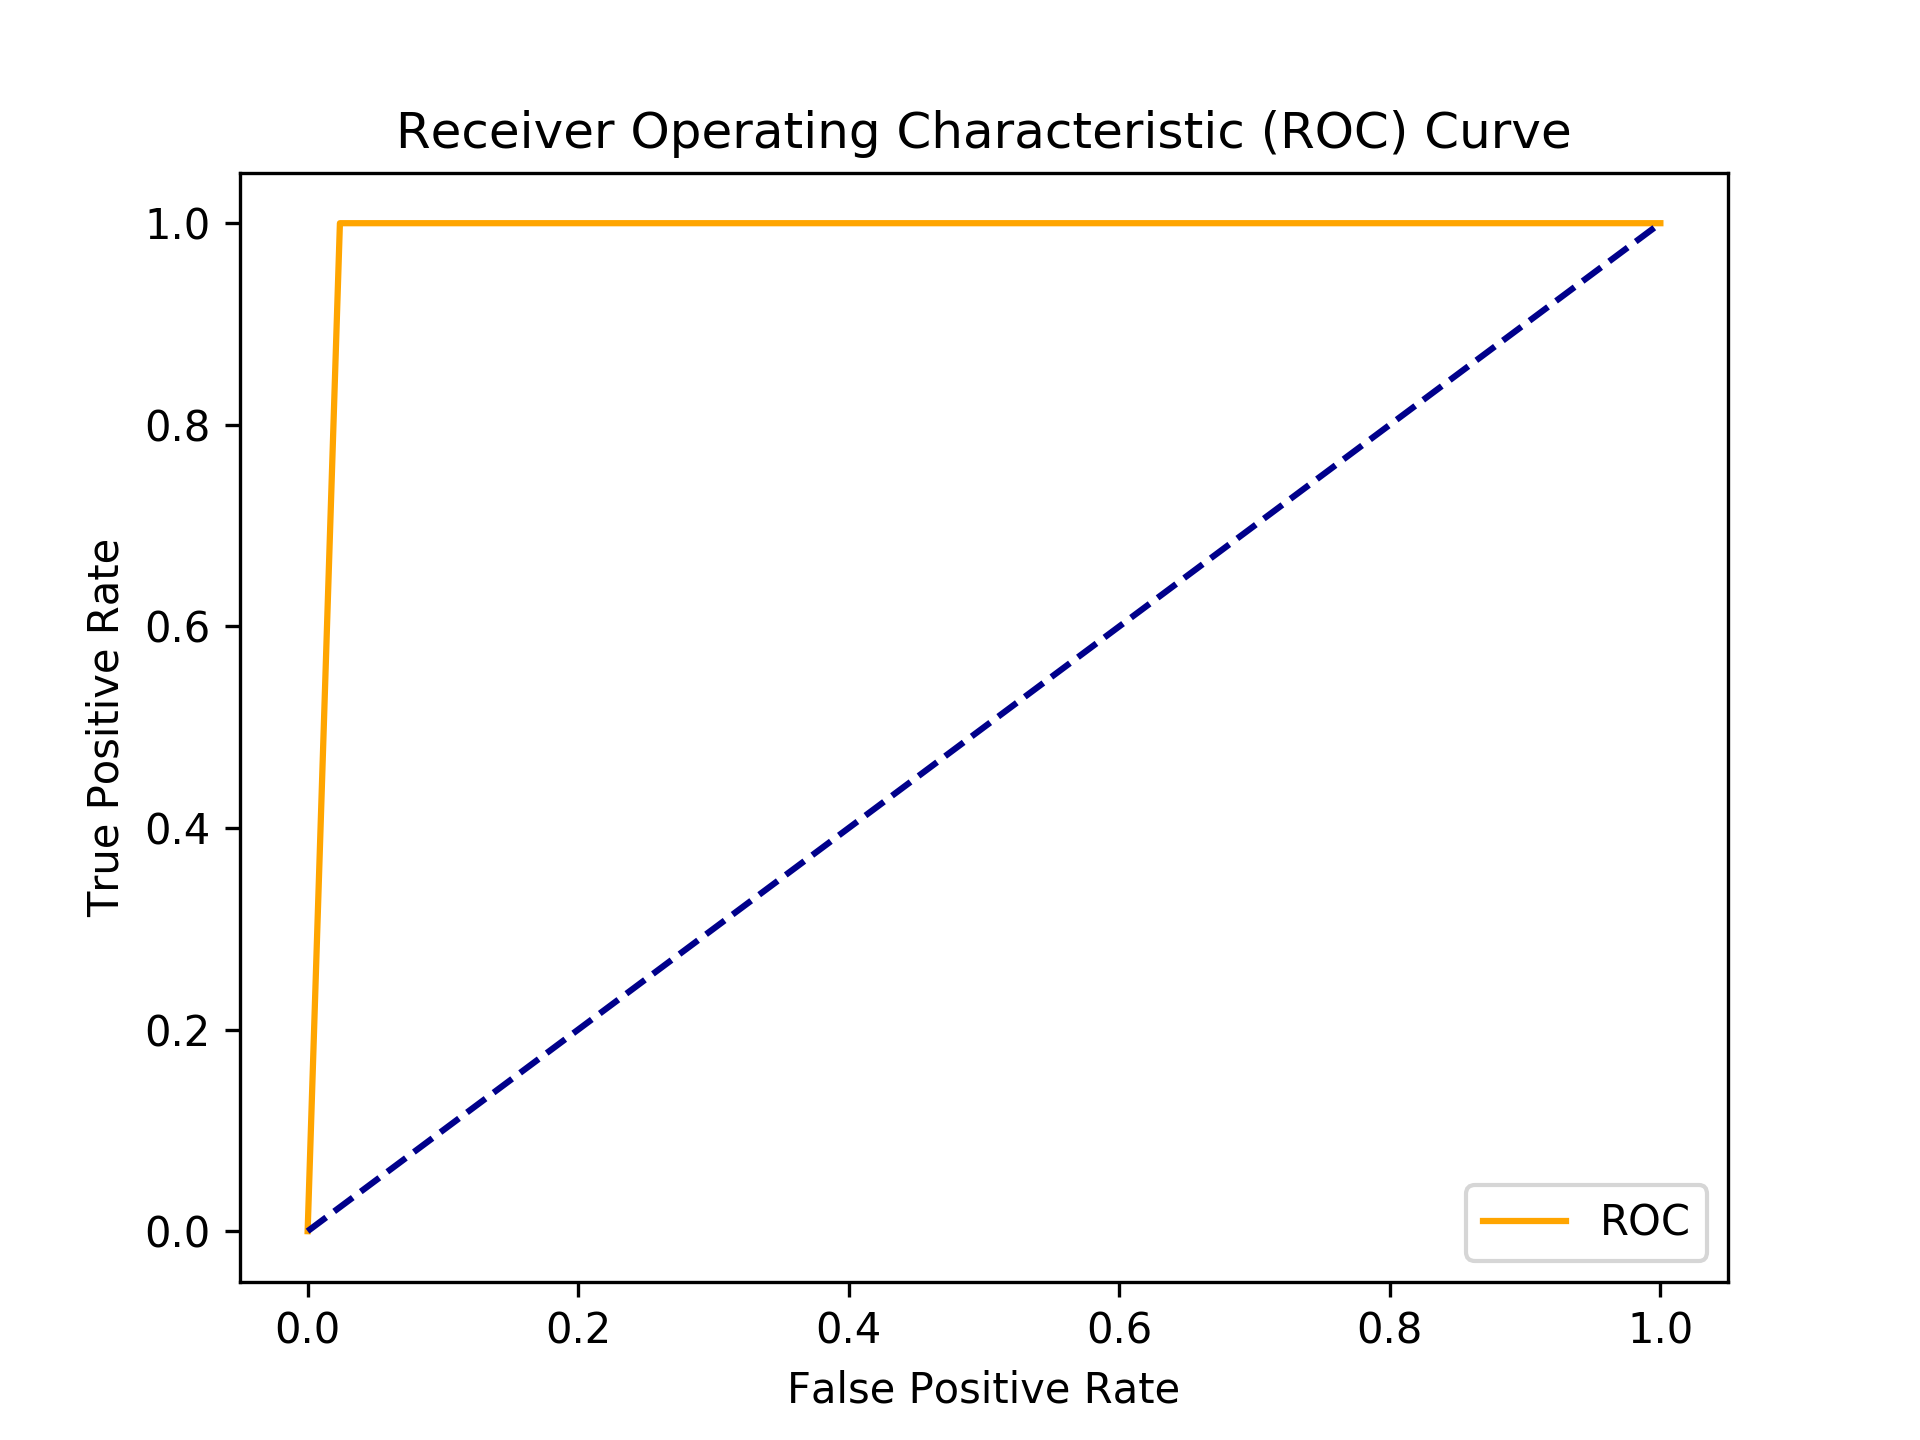
\includegraphics[trim={1cm 0.5cm 0cm 1cm}, width=0.322\textwidth]{results/transfer/roc_curve_transfer_multiclass_bert_0.15.png}}
\hspace{\fill}
   \subfloat[GPT-2\label{fig:roc_curve_gpt_transfer_multiclass} ]{%
      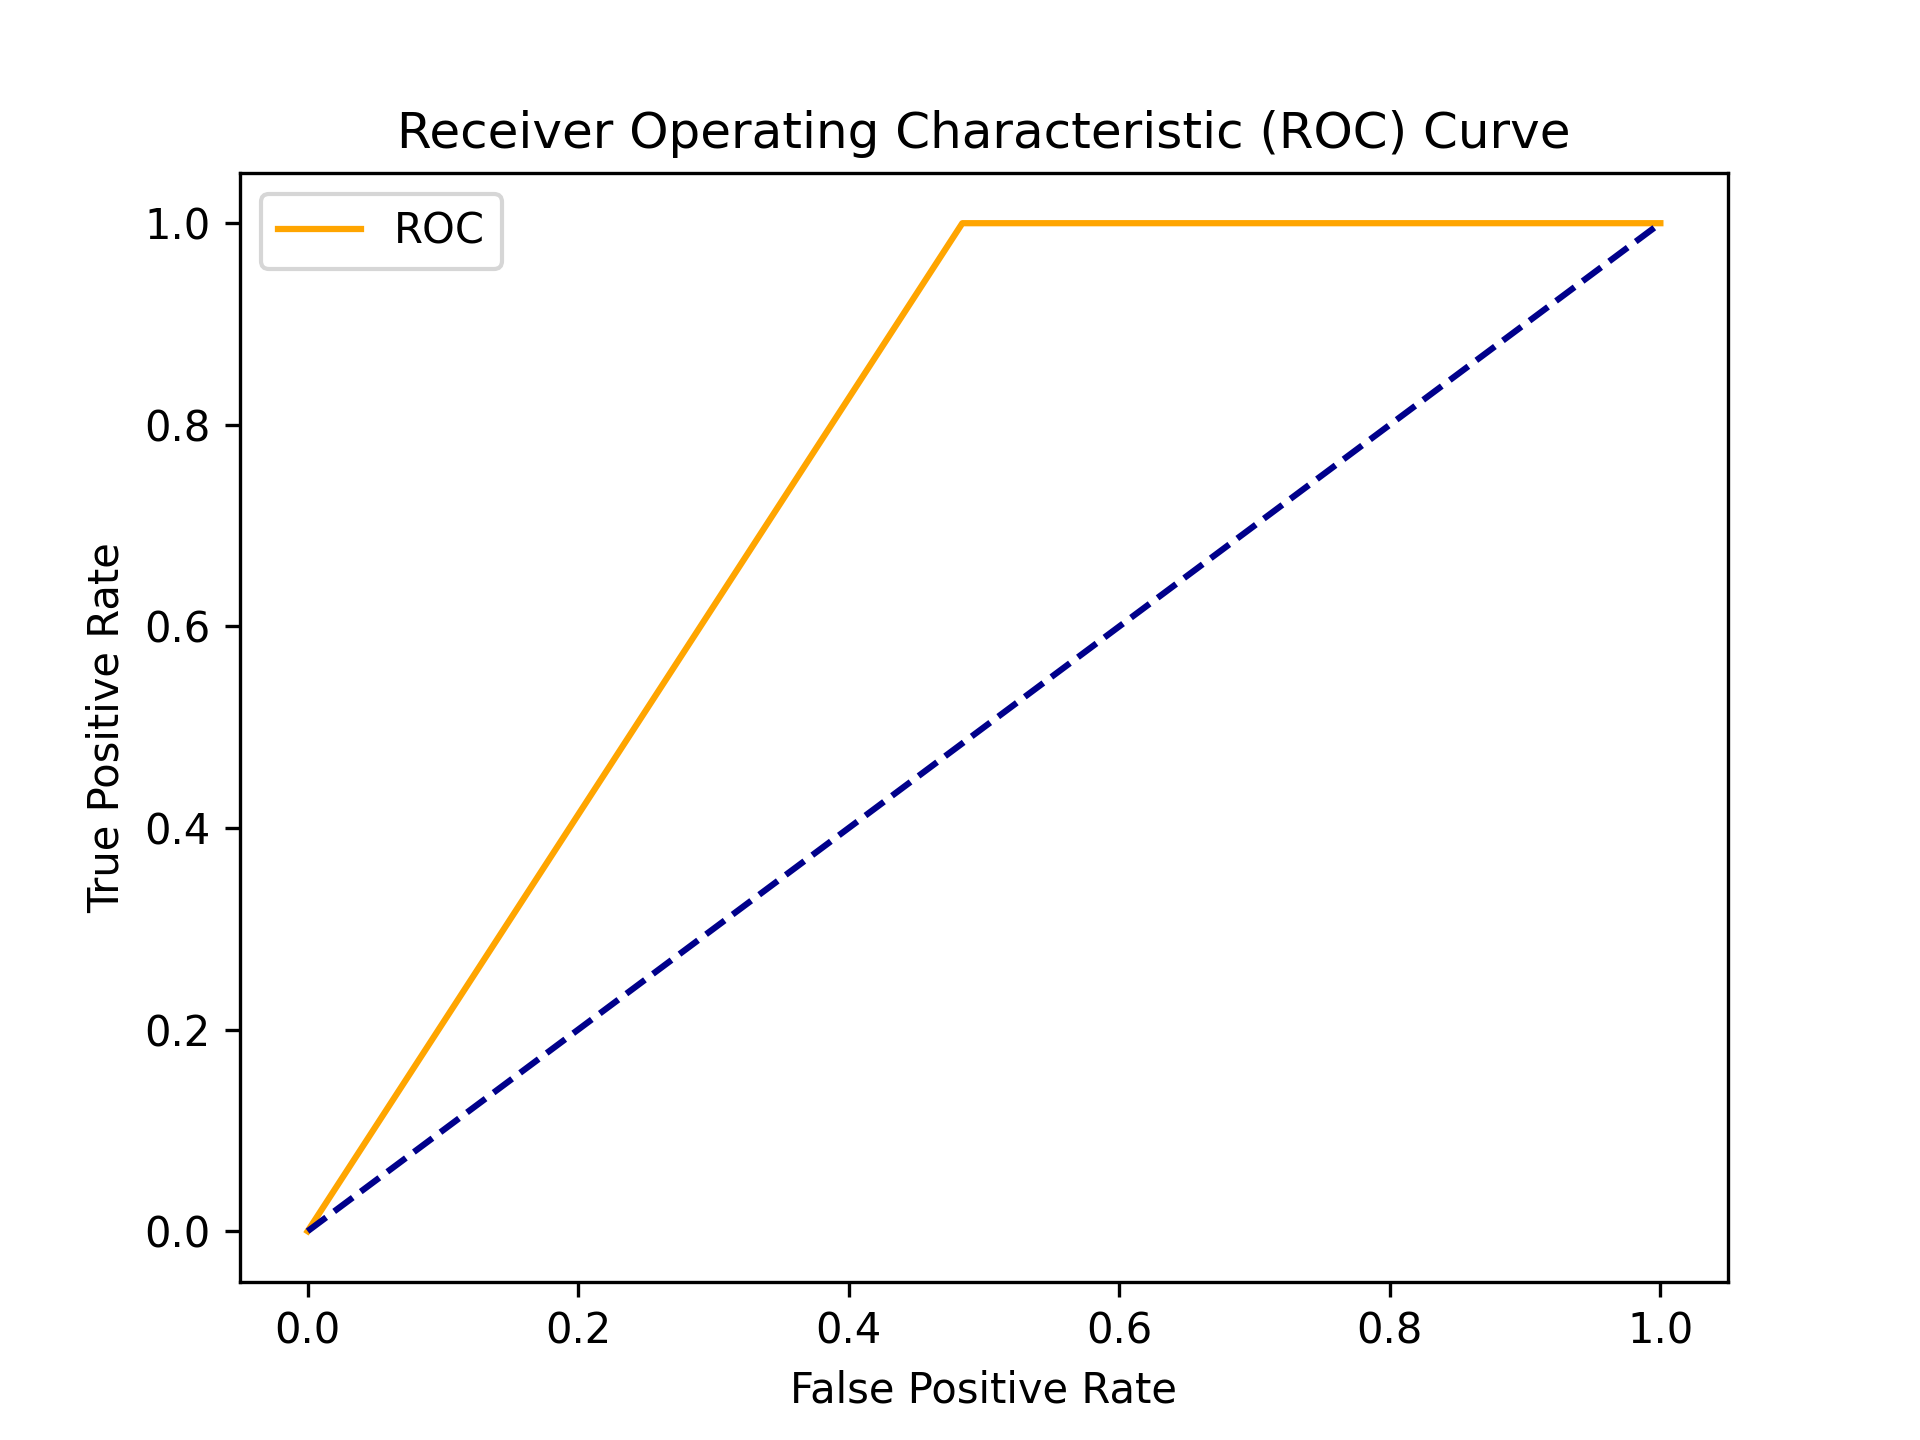
\includegraphics[trim={1cm 0.5cm 0cm 1cm}, width=0.322\textwidth]{results/transfer/roc_curve_transfer_multiclass_gpt_0.15.png}}
\hspace{\fill}
   \subfloat[XL\label{fig:roc_curve_xl_transfer_multiclass}]{%
      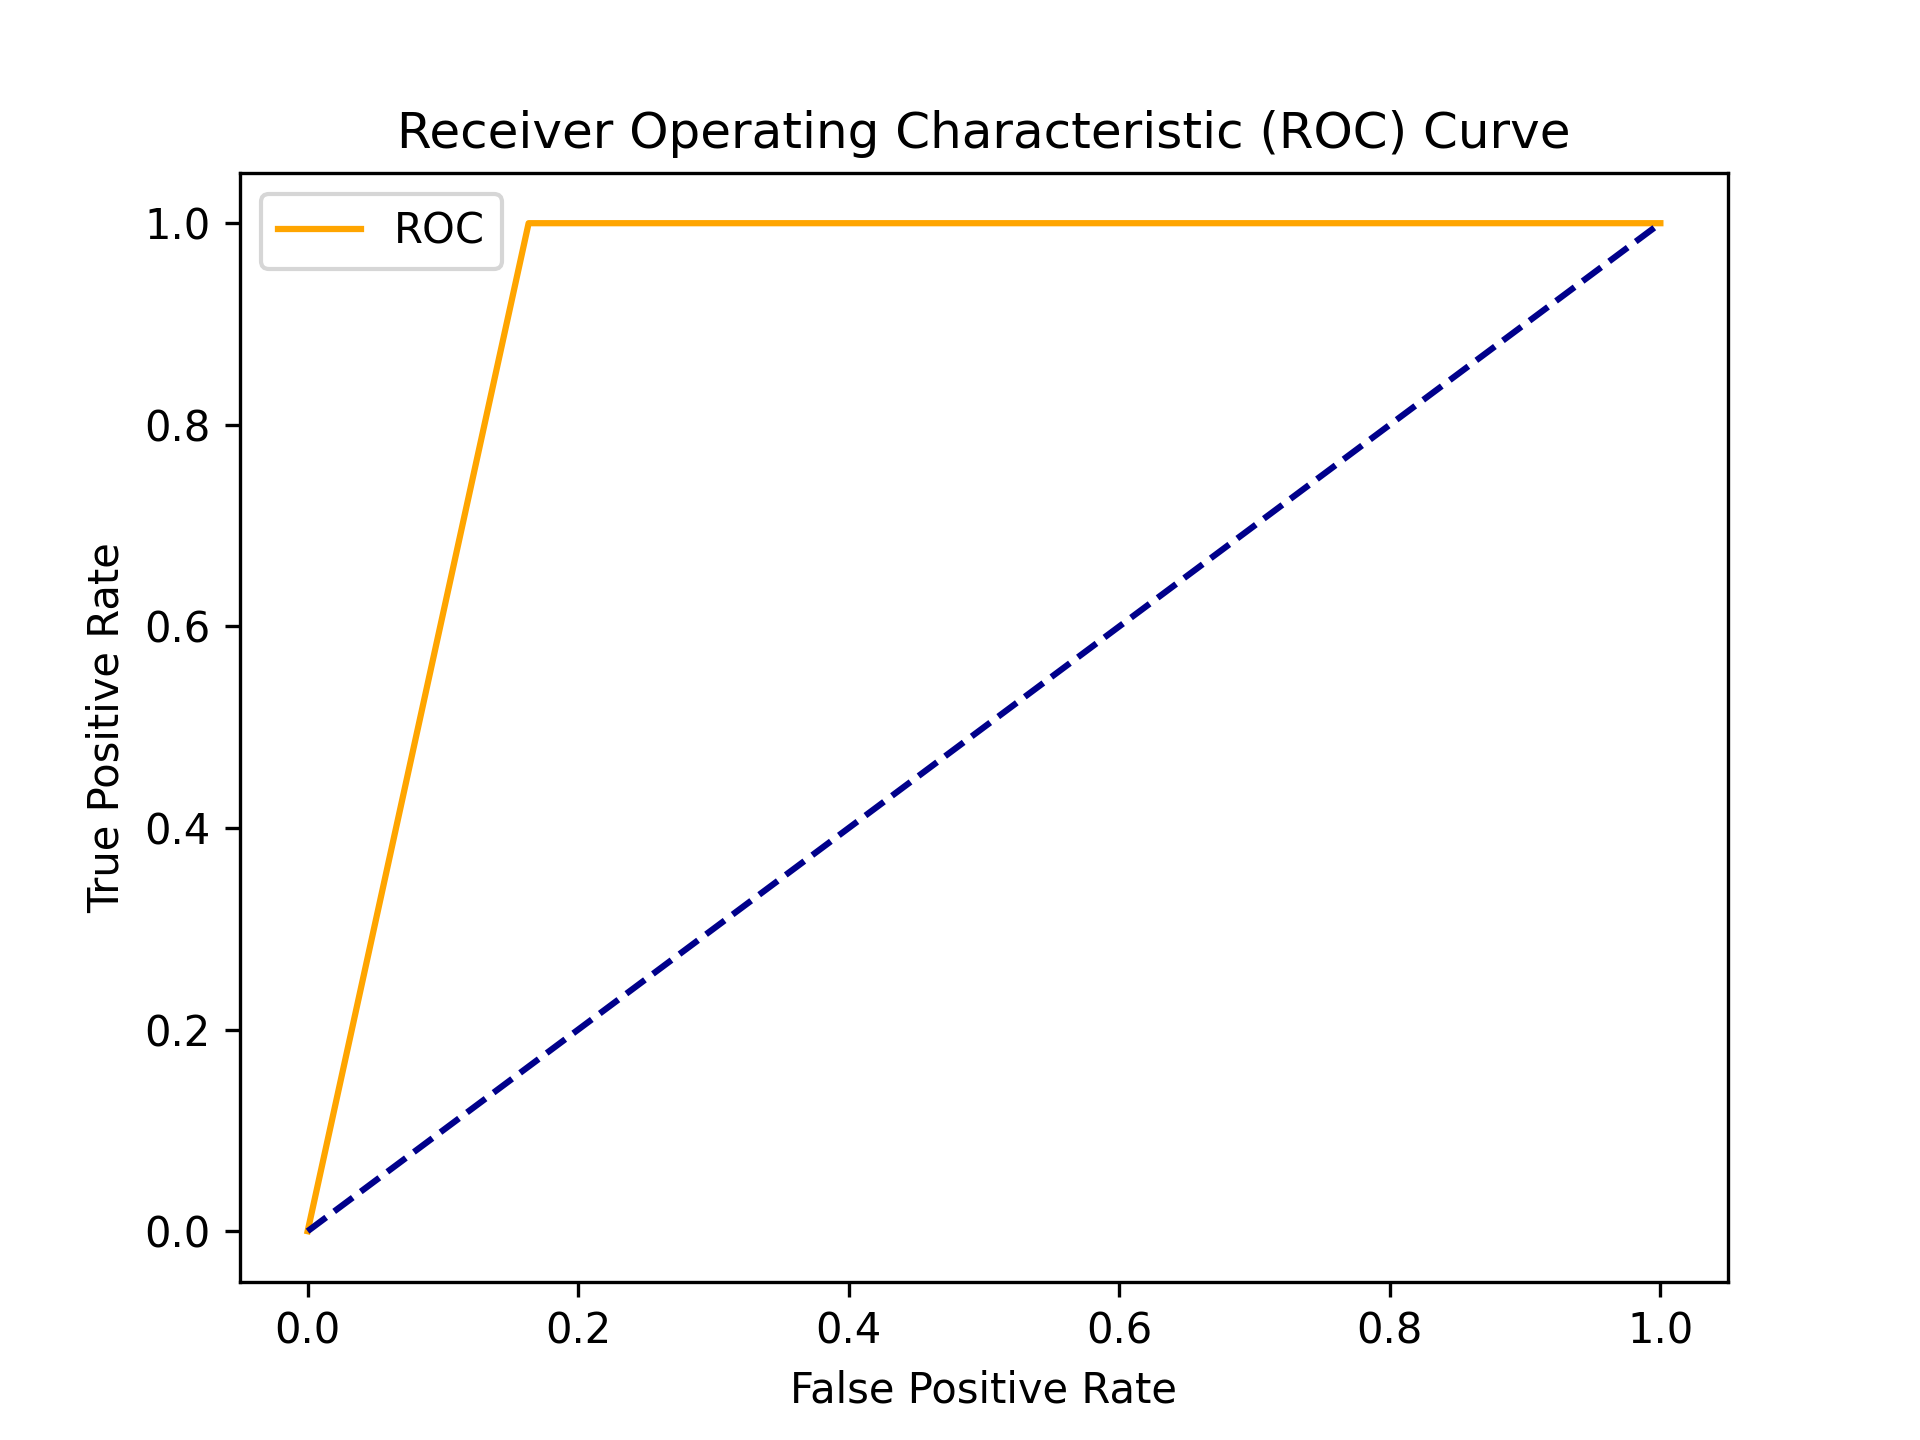
\includegraphics[trim={1cm 0.5cm 0cm 1cm}, width=0.322\textwidth]{results/transfer/roc_curve_transfer_multiclass_xl_0.15.png}}\\
\caption{\label{fig:results_transfer_multiclass_roc}ROC-Curve for transfer of knowledge using regression with 15\% alterations.}
\end{figure*}
\clearpage
\begin{figure}[h]
  \centering
  \captionsetup{justification=centering}
  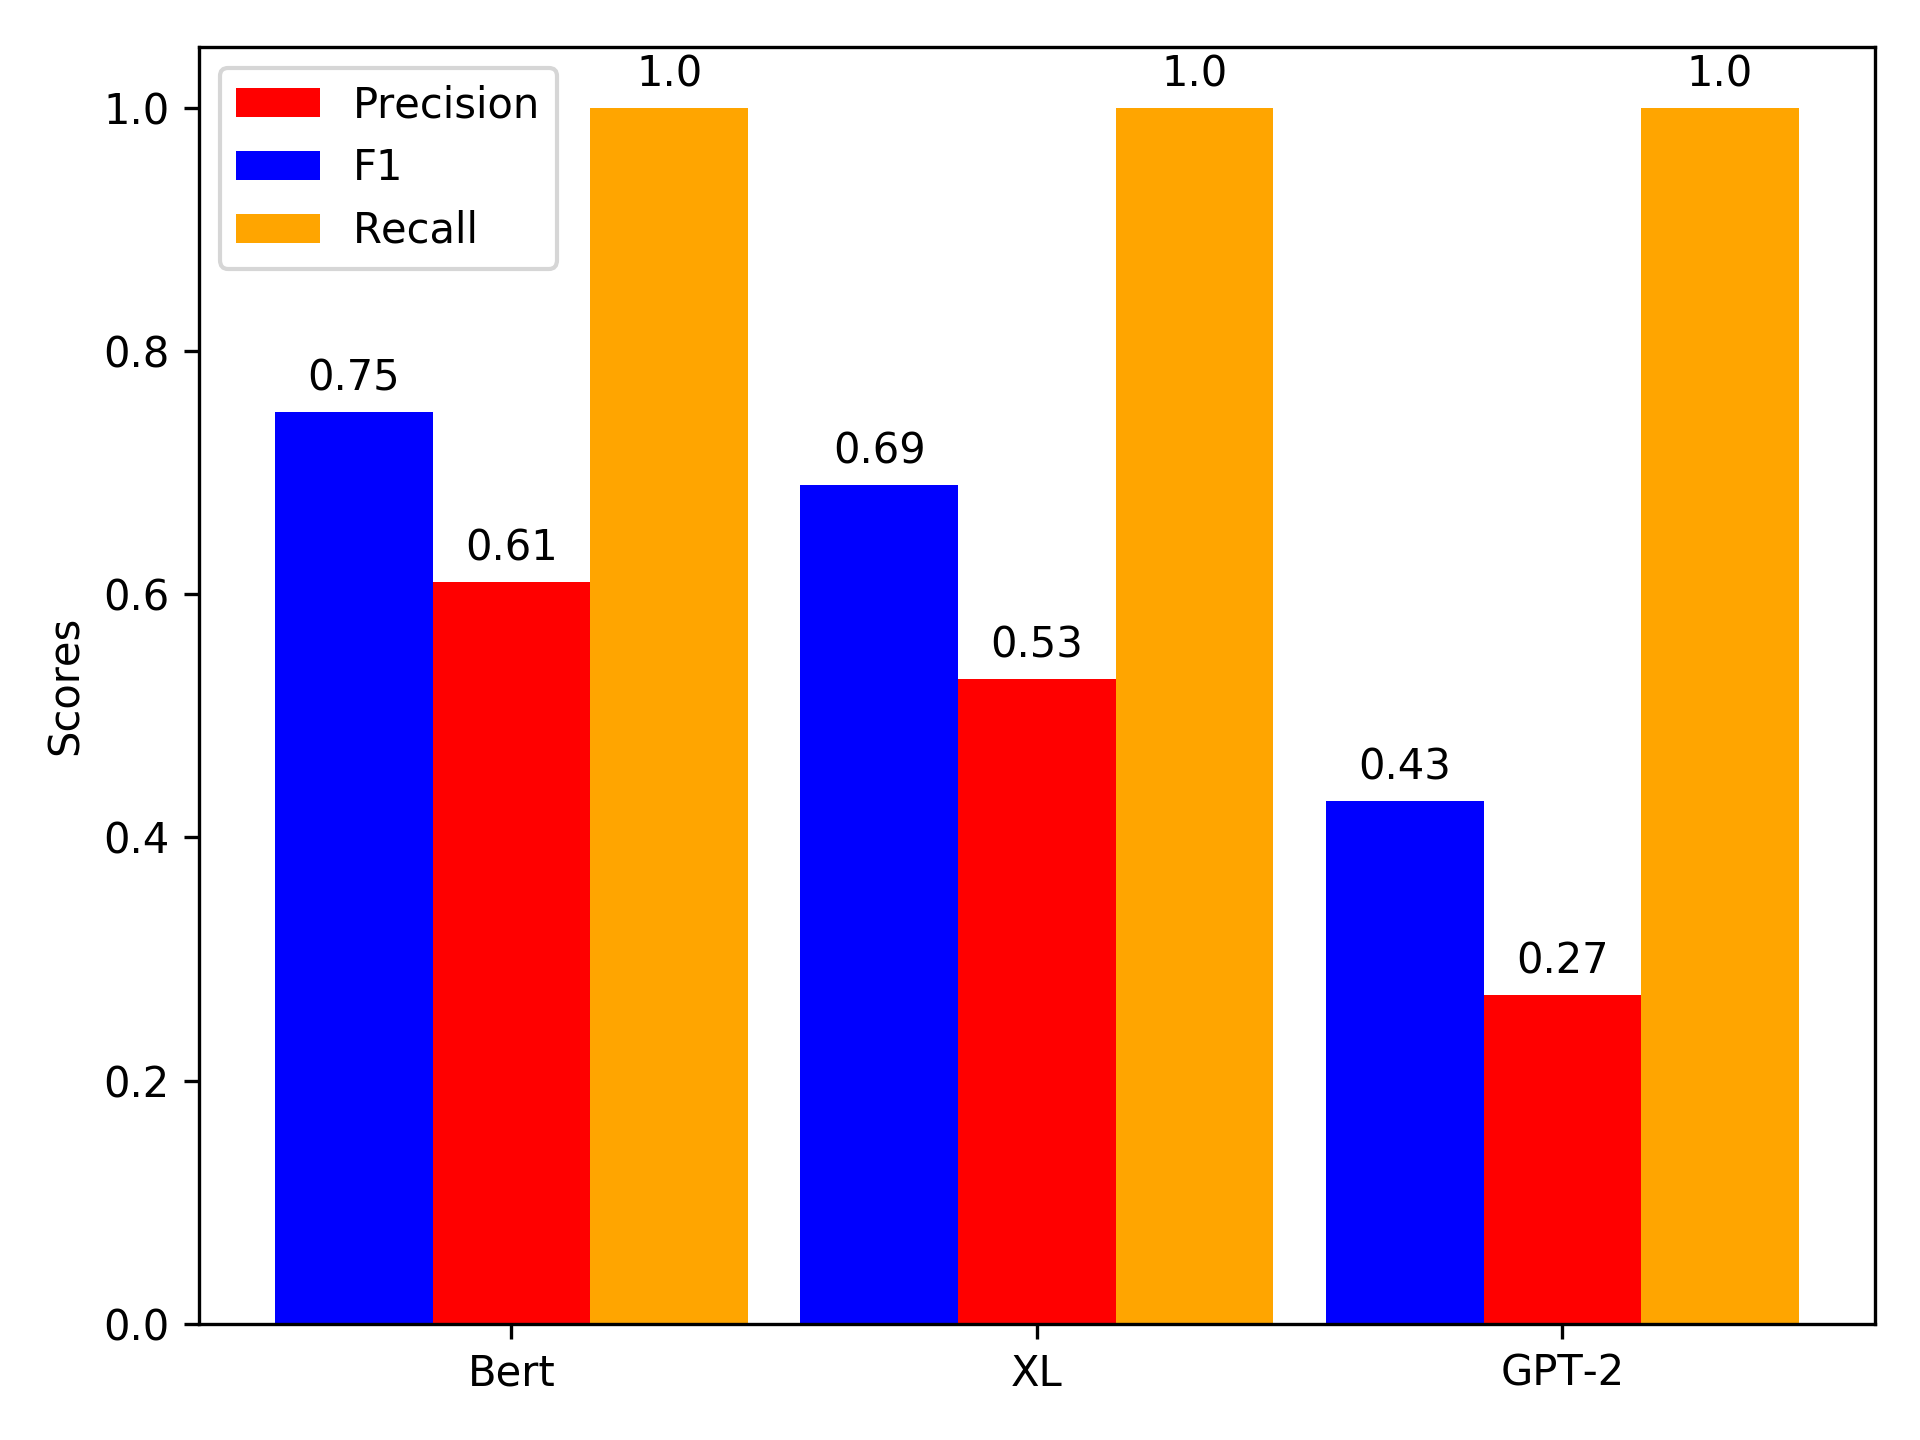
\includegraphics[width=8cm]{results/transfer_multiclass_replace_half.png}\\
  \caption{Transfer of knowledge. For 15\% of lines, replace 50\% of words, mark as anomaly, using classification.}
  \label{fig:replace_words_classification_transfer}
\end{figure}


\section{Discussion of Results\label{sec:discussion_results}}
By evaluating three different language models, it has been shown that the used word embeddings can highly influence the quality of the results for anomaly detection, with different word embeddings having strengths and weaknesses in different categories. 

\begin{comment}
For anomaly detection on one dataset using the regression approach, GPT-2 shows strong results, with F1-Scores of 0.95 when altering 5\% of log sequences, and 0.93 when altering the log lines, the quality of the results don't degrade much, when alteration ratios are increased, where Bert and XL-Transformers show decreases of 0.1 to 0.2 percentage points when increasing the alteration ratio from 5\% to 15\%. Yet, when the log events are completely reversed, GPT-2 achieves an F1-Score of only 0.55, where Bert and XL achieve 0.98, almost perfectly detecting the wrong sequence of log events.
\end{comment}

For the regression-based approach on one dataset, GPT-2 beats Bert and XL-Transformers clearly with regards to all metrics, achieving an F1-score of 0.94 and recall of 1.0, for injecting alterations on 15\% of the sequences of logs, where Bert achieves 0.56 F1-score and recall of 1.0 and XL-Transformers only achieves 0.31 F1-score and 0.64 recall. Similar results can be seen for the alterations of log lines, where Bert and XL-Transformers improve by around 10 percentage points, while GPT-2 degrades by around 8 percentage points.

For the classification-based approach on one dataset on the other hand, GPT-2 shows weaker results than Bert and XL-Transformers, with Bert being ahead of XL-Transformers and GPT-2 in all categories. For injecting alterations on 15\% of the sequences of logs Bert returns a F1-score of 0.54 and recall of 1.0, XL-Transformers returns a F1-score of 0.41 and recall of 1.0, and GPT-2 returns a F1-score of 0.36 and recall of 0.7. For altering of log events, the F1-score of Bert is 13 percentage points better, for XL-Transformers it is 12 percentage points better, and for GPT only 7 percentage points better, while recall stays unchanged for all.

For the transfer of knowledge approach, the results show a different picture. Using the regression approach, GPT-2 is still ahead of the other two, returning a F1-score of 0.97 and recall of 1.0, while Bert achieves a F1-score of 0.68 and recall of 1.0, and finally XL-Transformers delivering again the least promising results of all three with a F1-score of 0.26 and recall of 0.47 for 15\% alteration ratio. 

On the other hand, for transfer of knowledge using the classification-based approach, for 15\% alteration, GPT-2 shows results that are not very promising, while still being able to find all anomalies, but showing a small F1-Score of only 0.17, where Bert is able to reach a F1-Score of 0.81 and XL-Transformers achieving 0.38. It is also visible, that GPT-2 seems to not profit as much from the few-shot learning on the new training dataset, where the metrics stay almost the same throughout between epochs 1 and 5, yet Bert shows improvements from an F1-Score of 0.3 to 0.8 between epoch 1 and 5. It can be summarised that Bert is the best of the three language models for classification and GPT-2 is the best language model for the regression-based approach.

%It is evident, that with more hyperparameter-tuning, far better results can be accomplished, especially with XL-Transformers, since it obviously requires a different setup of hidden units and layers within the LSTM to achieve optimal results, however, since the model is a prototype and is supposed to show the possibility of comparing different word embeddings, not all potentials were fully tapped.

%TODO box plots of loss values in 